% ------------------------------------------------------------------------
% ------------------------------------------------------------------------
% Modelo UFSC para Trabalhos Academicos (tese de doutorado, dissertação de
% mestrado) utilizando a classe abntex2
%
% Autor: Alisson Lopes Furlani
% 	Modificações:
%	- 27/08/2019: Alisson L. Furlani, add pacote 'glossaries' para listas
%   - 06/11/2019: Luiz-Rafael Santos, modifica para Trabalho de Conclusão de Curso
% ------------------------------------------------------------------------
% ------------------------------------------------------------------------

\documentclass[
	% -- opções da classe memoir --
	12pt,				% tamanho da fonte
	%openright,			% capítulos começam em pág ímpar (insere página vazia caso preciso)
	oneside,			% para impressão no anverso. Oposto a twoside
	a4paper,			% tamanho do papel. 
	% -- opções da classe abntex2 --
	chapter=TITLE,		% títulos de capítulos convertidos em letras maiúsculas
	section=TITLE,		% títulos de seções convertidos em letras maiúsculas
	%subsection=TITLE,	% títulos de subseções convertidos em letras maiúsculas
	%subsubsection=TITLE,% títulos de subsubseções convertidos em letras maiúsculas
	% -- opções do pacote babel --
	english,			% idioma adicional para hifenização
	%french,				% idioma adicional para hifenização
	%spanish,			% idioma adicional para hifenização
	brazil				% o último idioma é o principal do documento
	]{abntex2}

\usepackage{setup/ufscthesisA4-alf}

% ---
% Filtering and Mapping Bibliographies
% ---
% Pacotes de citações
% ---
\usepackage{csquotes}
\usepackage{float}
\usepackage{mathtools}
\usepackage[backend = biber, style = abnt]{biblatex}
\usepackage{subcaption}
\newcommand\ddfrac[2]{\frac{\displaystyle #1}{\displaystyle #2}}
% FIXME Se desejar estilo numérico de citações,  comente a linha acima e descomente a linha a seguir.
% \usepackage[backend = biber, style = numeric-comp]{biblatex}

\setlength\bibitemsep{\baselineskip}
\DeclareFieldFormat{url}{Disponível~em:\addspace\url{#1}}
\NewBibliographyString{sineloco}
\NewBibliographyString{sinenomine}
\DefineBibliographyStrings{brazil}{%
	sineloco     = {\mkbibemph{S\adddot l\adddot}},
	sinenomine   = {\mkbibemph{s\adddot n\adddot}},
	andothers    = {\mkbibemph{et\addabbrvspace al\adddot}},
	in			 = {\mkbibemph{In:}}
}

\addbibresource{aftertext/references.bib} % Seus arquivos de referências

% ---
\DeclareSourcemap{
	\maps[datatype=bibtex]{
		% remove fields that are always useless
		\map{
			\step[fieldset=abstract, null]
			\step[fieldset=pagetotal, null]
		}
		% remove URLs for types that are primarily printed
%		\map{
%			\pernottype{software}
%			\pernottype{online}
%			\pernottype{report}
%			\pernottype{techreport}
%			\pernottype{standard}
%			\pernottype{manual}
%			\pernottype{misc}
%			\step[fieldset=url, null]
%			\step[fieldset=urldate, null]
%		}
		\map{
			\pertype{inproceedings}
			% remove mostly redundant conference information
			\step[fieldset=venue, null]
			\step[fieldset=eventdate, null]
			\step[fieldset=eventtitle, null]
			% do not show ISBN for proceedings
			\step[fieldset=isbn, null]
			% Citavi bug
			\step[fieldset=volume, null]
		}
	}
}
% ---

% ---
% Informações de dados para CAPA e FOLHA DE ROSTO
% ---
% FIXME Substituir 'Nome completo do autor' pelo seu nome.
\autor{Deiwid Decker Hoffer}
% FIXME Substituir 'Título do trabalho' pelo título da trabalho.
\titulo{Uma revisão sobre a simulação computacional do impacto balístico.}
% FIXME Substituir 'Subtítulo (se houver)' pelo subtítulo da trabalho.  
% Caso não tenha substítulo, comente a linha a seguir.
%\subtitulo{Subtítulo (se houver)}
% FIXME Substituir 'XXXXXX' pelo nome do seu
% orientador.
\orientador{Prof. Marcio Celso Fredel, Dr.}
% FIXME Se for orientado por uma mulher, comente a linha acima e descomente a linha a seguir.
% \orientador[Orientadora]{Nome da orientadora, Dra.}
% FIXME Substituir 'XXXXXX' pelo nome do seu
% coorientador. Caso não tenha coorientador, comente a linha a seguir.
%\coorientador{Prof. XXXXXX, Dr.}
% FIXME Se for coorientado por uma mulher, comente a linha acima e descomente a linha a seguir.
% \coorientador[Coorientadora]{XXXXXX, Dra.}
% FIXME Substituir 'XXXXXX' pelo nome do Coordenador do 
% programa/curso.
\coordenador{Prof. Celso Peres, Dr.}
% FIXME Se for coordenadora mulher, comente a linha acima e descomente a linha a seguir.
% \coordenador[Coordenadora]{Nome da Coordenadora, Dra.}
% FIXME Substituir '[ano da entrega]' pelo ano (ano) em que seu trabalho foi defendido.
\ano{2020}
% FIXME Substituir '[dia] de [mês] de [ano]' pela data em que ocorreu sua defesa.
\data{[dia] de [mês] de 2020}
% FIXME Substituir '[Cidade da defesa]' pela cidade em que ocorreu sua defesa.
\local{Florianópolis}
\instituicaosigla{UFSC}
\instituicao{Universidade Federal de Santa Catarina}
% FIXME Substituir 'Dissertação/Tese' pelo tipo de trabalho (Tese, Dissertação). 
\tipotrabalho{Trabalho de Conclusão de Curso}
% FIXME Substituir '[licenciado/bacharel] em [nome do título obtido]' pela grau adequado.
\formacao{bacharel em Engenharia de Materiais}
% FIXME Substituir '[licenciado/bacharel]' pelo nivel adequado.
\nivel{bacharel}
% FIXME Substituir 'Curso de Graduação em [XXXXXXXX]' pela curso adequado.
\programa{Curso de Graduação em Engenharia de Materiais}
% FIXME Substituir 'Campus XXXXXX ou Centro de XXXXXX' pelo campus ou centro adequado.
\centro{Centro Tecnológico}
\preambulo
{%
\imprimirtipotrabalho~do~\imprimirprograma~do~\imprimircentro~da~\imprimirinstituicao~para~a~obtenção~do~título~de~\imprimirformacao.
}
% ---

% ---
% Configurações de aparência do PDF final
% ---
% alterando o aspecto da cor azul
\definecolor{blue}{RGB}{41,5,195}
% informações do PDF
\makeatletter
\hypersetup{
     	%pagebackref=true,
		pdftitle={\@title}, 
		pdfauthor={\@author},
    	pdfsubject={\imprimirpreambulo},
	    pdfcreator={LaTeX with abnTeX2},
		pdfkeywords={ufsc, latex, abntex2}, 
		colorlinks=true,       		% false: boxed links; true: colored links
    	linkcolor=black,%blue,          	% color of internal links
    	citecolor=black,%blue,        		% color of links to bibliography
    	filecolor=black,%magenta,      		% color of file links
		urlcolor=black,%blue,
		bookmarksdepth=4
}
\makeatother
% ---

% ---
% compila a lista de abreviaturas e siglas e a lista de símbolos
% ---

% Declaração das siglas
\siglalista{ABNT}{Associação Brasileira de Normas Técnicas}

% Declaração dos simbolos
\simbololista{pi}{\ensuremath{\pi}}{Número pi} 
\simbololista{r}{\ensuremath{r}}{Raio de um círculo}
\simbololista{A}{\ensuremath{A}}{Área de um círculo}
\simbololista{deltaK}{\ensuremath{\delta_{ij}}}{Símbolo de Kronecker Delta}
\simbololista{levicivita}{\ensuremath{\epsilon_{ijk}}}{Símbolo de Levi Civita}
\simbololista{E}{\ensuremath{E}}{Tensor deformação de Green-Lagrange}
\simbololista{C}{\ensuremath{C}}{Tensor deformação direito de Cauchy-Green}
\simbololista{B}{\ensuremath{B}}{Tensor deformação esquerdo de Cauchy-Green}
\simbololista{U}{\ensuremath{U}}{Tensor direito de estiramento}
\simbololista{V}{\ensuremath{V}}{Tensor esquerdo de estiramento}
\simbololista{F}{\ensuremath{F}}{Tensor gradiente da deformação}
\simbololista{H}{\ensuremath{H}}{Tensor gradiente do deslocamento}
\simbololista{eps}{\ensuremath{\varepsilon}}{Tensor deformação infinitesimal}
\simbololista{R}{\ensuremath{R}}{Tensor rotação}
\simbololista{rho}{\ensuremath{\rho}}{Densidade do corpo na configuração espacial}
\simbololista{rhor}{\ensuremath{\rho_r}}{Densidade do corpo na configuração material}
\simbololista{Omegar}{\ensuremath{\Omega_r}}{Região ocupada pelo corpo na configuração material}
\simbololista{Omega}{\ensuremath{\Omega}}{Região ocupada pelo corpo na configuração espacial}
\simbololista{t}{\ensuremath{\boldsymbol{t}}}{Força de superfície}
\simbololista{b}{\ensuremath{\boldsymbol{b}}}{Força de corpo}
\simbololista{Cauchy}{\ensuremath{\boldsymbol{\sigma}}}{Tensor de tensões de Cauchy}
\simbololista{P}{\ensuremath{\boldsymbol{P}}}{Primeiro tensor de tensões de Piola-Kirchhoff}
\simbololista{e_r}{\ensuremath{e_r}}{Energia interna do corpo na configuração material}
\simbololista{K}{\ensuremath{\mathcal{K}(\Omega_r)}}{Energia cinética do corpo na configuração material}
\simbololista{convpower}{\ensuremath{\mathcal{W}_0(\Omega_r)}}{Potência externa aplicada ao corpo na configuração material}
\simbololista{Pint}{\ensuremath{\mathcal{P}_{int}(\Omega_r)}}{Potência interna do corpo na configuração material}
\simbololista{Etot}{\ensuremath{\mathcal{E}_{tot}(\Omega_r)}}{Energia total do corpo na configuração material}
\simbololista{Q}{\ensuremath{\mathcal{Q}(\Omega_r)}}{Fluxo de calor na configuração material}
\simbololista{I}{\ensuremath{\boldsymbol{I}}}{Tensor identidade}
\simbololista{printens}{\ensuremath{\sigma_i}}{Tensões principais}
\simbololista{prinvadesv}{\ensuremath{J_i}}{Invariantes do tensor de tensões desviadoras}
\simbololista{prinva}{\ensuremath{I_i}}{Invariantes do tensor de tensões}
\simbololista{N}{\ensuremath{\boldsymbol{N}}}{Vetor fluxo plástico}
\simbololista{gamma}{\ensuremath{\dot{\gamma}}}{multiplicador plástico}
\simbololista{defplastacu}{\ensuremath{ \overline{\varepsilon}^p }}{Deformação plástica acumulada}
\simbololista{hugoniot}{\ensuremath{\sigma_{LEH}}}{Limite elástico de Hugoniot}
\simbololista{u}{\ensuremath{\boldsymbol{u}}}{Campo vetorial de deslocamentos do corpo}
\simbololista{uvir}{\ensuremath{\boldsymbol{\hat{u}}}}{Campo vetorial de deslocamentos virtuais do corpo}


% compila a lista de abreviaturas e siglas e a lista de símbolos
\makenoidxglossaries 

% ---

% ---
% compila o indice
% ---
\makeindex
% ---

% ----
% Início do documento
% ----
\begin{document}

% Seleciona o idioma do documento (conforme pacotes do babel)
%\selectlanguage{english}
\selectlanguage{brazil}

% Retira espaço extra obsoleto entre as frases.
\frenchspacing 

% Espaçamento 1.5 entre linhas
\OnehalfSpacing

% Corrige justificação
%\sloppy

% ----------------------------------------------------------
% ELEMENTOS PRÉ-TEXTUAIS
% ----------------------------------------------------------
% \pretextual %a macro \pretextual é acionado automaticamente no início de \begin{document}
% ---
% Capa, folha de rosto, ficha bibliografica, errata, folha de apróvação
% Dedicatória, agradecimentos, epígrafe, resumos, listas
% ---
% ---
% Capa
% ---
\imprimircapa
% ---

% ---
% Folha de rosto
% (o * indica que haverá a ficha bibliográfica)
% ---
\imprimirfolhaderosto*
% ---

% ---
% Inserir a ficha bibliografica
% ---
% http://ficha.bu.ufsc.br/
\begin{fichacatalografica}
	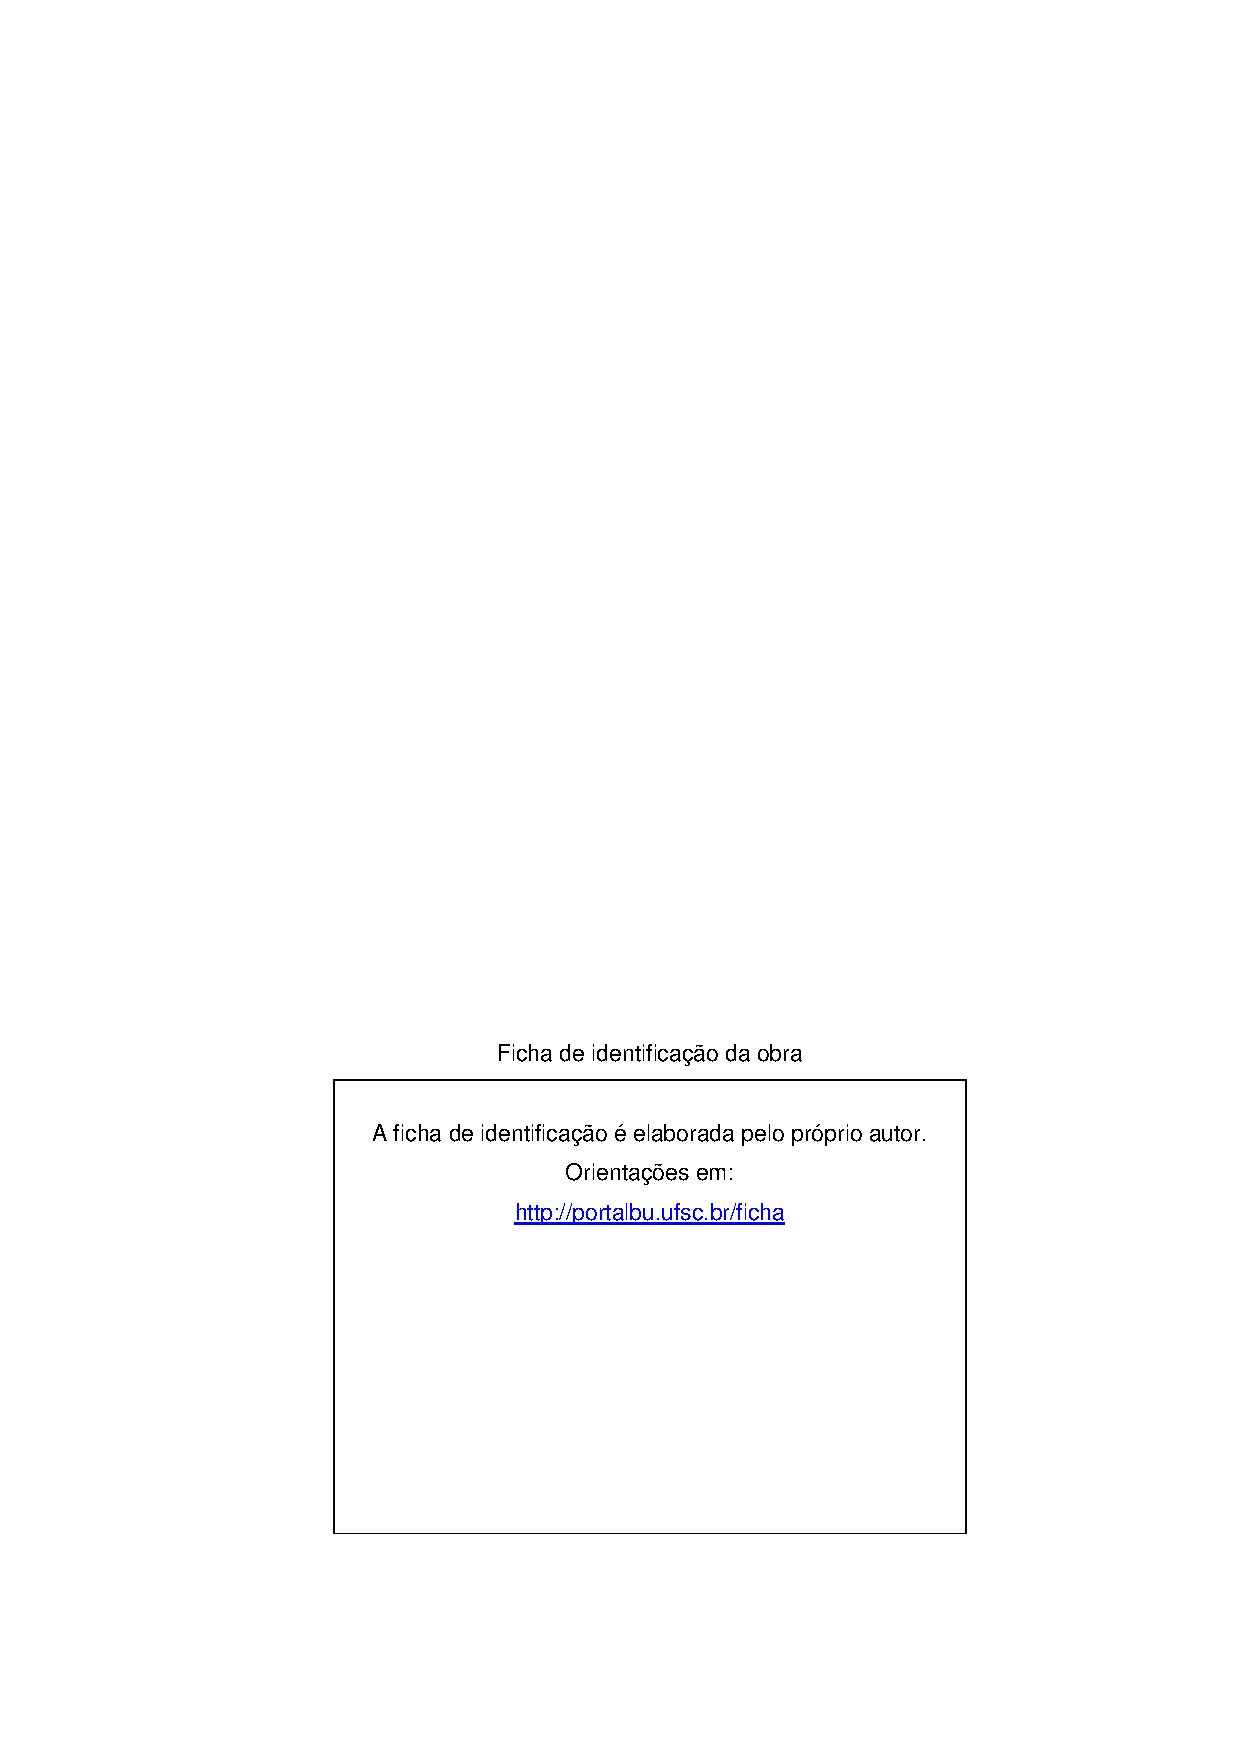
\includepdf{beforetext/Ficha_Catalografica.pdf}
\end{fichacatalografica}
% ---

% ---
% Inserir folha de aprovação
% ---
\begin{folhadeaprovacao}
	\OnehalfSpacing
	\centering
	\imprimirautor\\%
	\vspace*{10pt}		
	\textbf{\imprimirtitulo}%
	\ifnotempty{\imprimirsubtitulo}{:~\imprimirsubtitulo}\\%
	%		\vspace*{31.5pt}%3\baselineskip
	\vspace*{\baselineskip}
	%\begin{minipage}{\textwidth}
	% ~do~\imprimirprograma~do~\imprimircentro~da~\imprimirinstituicao~para~a~obtenção~do~título~de~\imprimirformacao.
	Este~\imprimirtipotrabalho~foi julgado adequado para obtenção do Título de “\imprimirformacao” e aprovado em sua forma final pelo~\imprimirprograma. \\
		\vspace*{\baselineskip}
	\imprimirlocal, \imprimirdata. \\
	\vspace*{2\baselineskip}
	\assinatura{\OnehalfSpacing\imprimircoordenador \\ \imprimircoordenadorRotulo~do Curso}
	\vspace*{2\baselineskip}
	\textbf{Banca Examinadora:} \\
	\vspace*{\baselineskip}
	\assinatura{\OnehalfSpacing\imprimirorientador \\ \imprimirorientadorRotulo}
	%\end{minipage}%
	\vspace*{\baselineskip}
	\assinatura{ André Cabral, Me.\\
	Avaliador \\
	Instituição Universidade Federal de Santa Catarina}

	\vspace*{\baselineskip}
	\assinatura{Prof. Inserir nome do Cel eduardo, Dr.\\
	Avaliador \\
	Instituição Instituto Militar de Engenharia}


\end{folhadeaprovacao}
% ---

% ---
% Dedicatória
% ---
\begin{dedicatoria}
	\vspace*{\fill}
	\noindent
	\begin{adjustwidth*}{}{5.5cm}     
		Este trabalho é dedicado aos meus colegas de classe e aos meus queridos pais.
	\end{adjustwidth*}
\end{dedicatoria}
% ---

% ---
% Agradecimentos
% ---
\begin{agradecimentos}
	Inserir os agradecimentos aos colaboradores à execução do trabalho. 
	
	Xxxxxxxxxxxxxxxxxxxxxxxxxxxxxxxxxxxxxxxxxxxxxxxxxxxxxxxxxxxxxxxxxxxxxx. 
\end{agradecimentos}
% ---

% ---
% Epígrafe
% ---
\begin{epigrafe}
	\vspace*{\fill}
	\begin{flushright}
		\textit{``Texto da Epígrafe.\\
			Citação relativa ao tema do trabalho.\\
			É opcional. A epígrafe pode também aparecer\\
			na abertura de cada seção ou capítulo.\\
			Deve ser elaborada de acordo com a NBR 10520.''\\
			(Autor da epígrafe, ano)}
	\end{flushright}
\end{epigrafe}
% ---

% ---
% RESUMOS
% ---

% resumo em português
\setlength{\absparsep}{18pt} % ajusta o espaçamento dos parágrafos do resumo
\begin{resumo}
	\SingleSpacing
	No resumo são ressaltados o objetivo da pesquisa, o método utilizado, as discussões e os resultados com destaque apenas para os pontos principais. O resumo deve ser significativo, composto de uma sequência de frases concisas, afirmativas, e não de uma enumeração de tópicos. Não deve conter citações. Deve usar o verbo na voz ativa e na terceira pessoa do singular. O texto do resumo deve ser digitado, em um único bloco, sem espaço de parágrafo. O espaçamento entre linhas é simples e o tamanho da fonte é 12. Abaixo do resumo, informar as palavras-chave (palavras ou expressões significativas retiradas do texto) ou, termos retirados de thesaurus da área. Deve conter de 150 a 500 palavras. O resumo é elaborado de acordo com a NBR 6028.
	
	\textbf{Palavras-chave}: Palavra-chave 1. Palavra-chave 2. Palavra-chave 3.
\end{resumo}

% resumo em inglês
\begin{resumo}[Abstract]
	\SingleSpacing
	\begin{otherlanguage*}{english}
		Resumo traduzido para outros idiomas, neste caso, inglês. Segue o formato do resumo feito na língua vernácula. As palavras-chave traduzidas, versão em língua estrangeira, são colocadas abaixo do texto precedidas pela expressão “Keywords”, separadas por ponto.
		
		\textbf{Keywords}: Keyword 1. Keyword 2. Keyword 3.
	\end{otherlanguage*}
\end{resumo}

%% resumo em francês 
%\begin{resumo}[Résumé]
% \begin{otherlanguage*}{french}
%    Il s'agit d'un résumé en français.
% 
%   \textbf{Mots-clés}: latex. abntex. publication de textes.
% \end{otherlanguage*}
%\end{resumo}
%
%% resumo em espanhol
%\begin{resumo}[Resumen]
% \begin{otherlanguage*}{spanish}
%   Este es el resumen en español.
%  
%   \textbf{Palabras clave}: latex. abntex. publicación de textos.
% \end{otherlanguage*}
%\end{resumo}
%% ---

{%hidelinks
	\hypersetup{hidelinks}
	% ---
	% inserir lista de ilustrações
	% ---
	\pdfbookmark[0]{\listfigurename}{lof}
	\listoffigures*
	\cleardoublepage
	% ---
	
	% ---
	% inserir lista de quadros
	% ---
	\pdfbookmark[0]{\listofquadrosname}{loq}
	\listofquadros*
	\cleardoublepage
	% ---
	
	% ---
	% inserir lista de tabelas
	% ---
	\pdfbookmark[0]{\listtablename}{lot}
	\listoftables*
	\cleardoublepage
	% ---
	
	% ---
	% inserir lista de abreviaturas e siglas (devem ser declarados no preambulo)
	% ---
	\imprimirlistadesiglas
	% ---
	
	% ---
	% inserir lista de símbolos (devem ser declarados no preambulo)
	% ---
	\imprimirlistadesimbolos
	% ---
	
	% ---
	% inserir o sumario
	% ---
	\pdfbookmark[0]{\contentsname}{toc}
	\tableofcontents*
	\cleardoublepage
	
}%hidelinks
% ---
% ---

% ----------------------------------------------------------
% ELEMENTOS TEXTUAIS
% ----------------------------------------------------------
\textual

% ---
% 1 - Introdução
% ---
% ----------------------------------------------------------
\chapter{Introdução}
% ----------------------------------------------------------

 O conceito de armadura é tão antigo quanto se possa imaginar. As armaduras tem acompanhado o ser humano através dos tempos. Sempre com o mesmo objetivo final, que é proteger recursos valiosos. Muitas vezes este recurso trata-se da própria vida de quem está sendo protegido pela armadura. Paul Hazell fala em seu livro, Armour Materials, Theory and Design, \cite{Hazell}, sobre o que chama de cebola da sobrevivência. Esta é uma analogia para as varias camadas da proteção, ver figura \ref{fig:0.1}.\\
 
 \begin{figure}[h]
 	\caption{Cebola da sobrevivência destacando a direita as camadas abordadas pelo trabalho.}
 	\centering
 	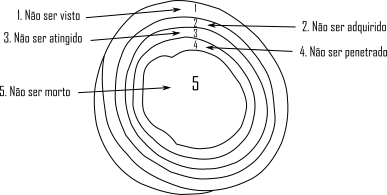
\includegraphics{images/cebola_sobrevive}
 	\label{fig:0.1}
 	\fonte{\cite{Hazell} traduzido pelo autor.}
 \end{figure}
O foco deste trabalho é revisar a fundamentação teórica da ferramenta mais usada para estudar a camada 4, não ser penetrado, que é a simulação computacional de impactos balísticos. Há certa interação entre não ser penetrado e não ser adquirido. Inicialmente parece enigmático o conceito de não ser adquirido, porém ele nada mais é do que a habilidade de poder escapar da mira humana ou de qualquer sistema de referenciação do projétil. Sendo assim quando se trata de veículos a velocidade é um dos maiores potencializadores da capacidade de não ser adquirido. \\

Um exemplo para a interação citada anteriormente pode ser dado usando veículos com motores a combustão interna. Os tanques são os veículos militares terrestres mais famosos na cultura popular. Em geral, quando comparados a outros veículos terrestres, os tanques tem o balanço desviado para a camada 4, não ser penetrado. Para cumprir sua função o tanque deve carregar munições e armas que quando somados possuem peso significativamente alto. Além disso é normal que o tanque tenha que assumir uma posição de apoio, logo deve permanecer em uma região específica. Somando as características e funções deste veículo, é natural que se construa um veículo com placas de metal espessas que suportem projeteis de energia cinética considerável. Tal construção gera um desequilíbrio em favor do tanque não ser penetrado, em detrimento dele não ser adquirido.\\ 

\begin{figure}[h]
	\caption{\label{fig:0.2} Veículo M1-Abrams}
	\centering
	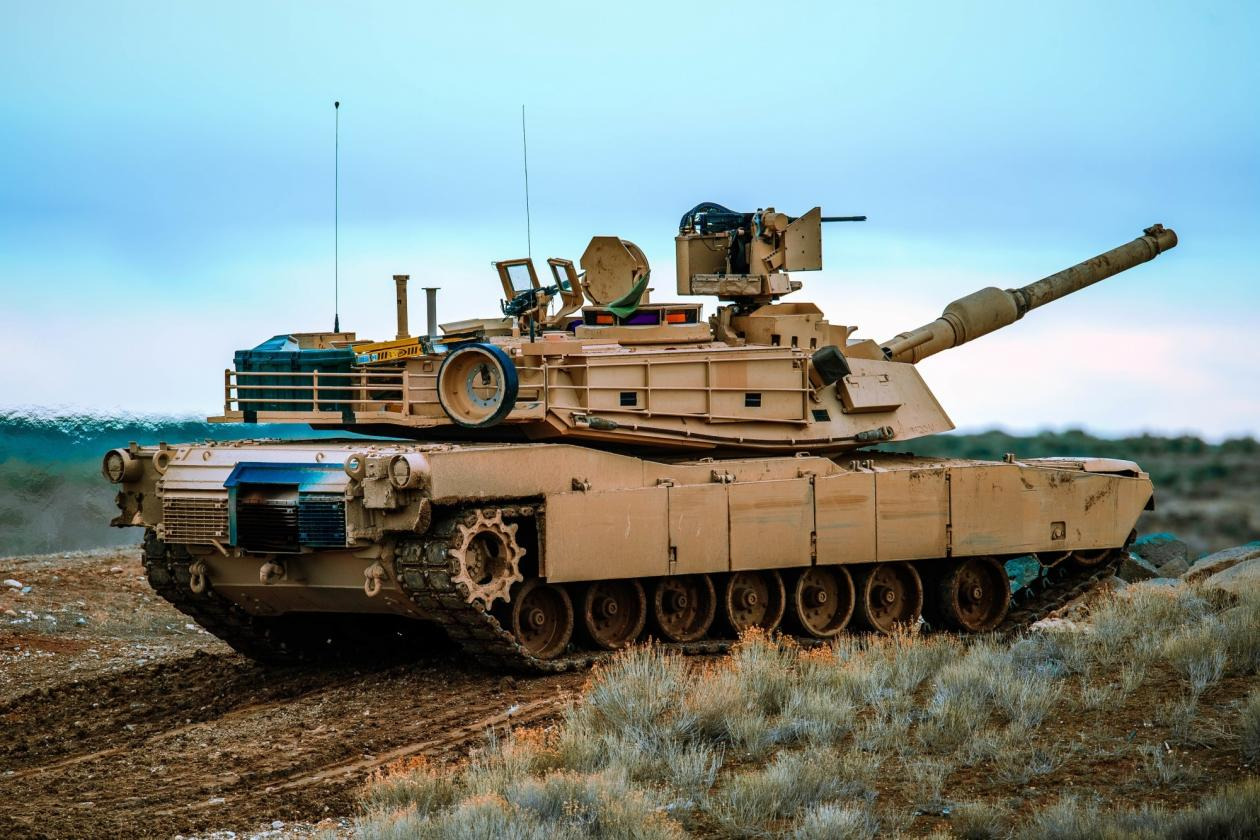
\includegraphics[width=0.7\linewidth]{images/m1-abrams}
	\fonte{https://nationalinterest.org/blog/buzz/us-armys-legendary-m1-abrams-tank-rip-or-ready-war-77621}
\end{figure}

 Do outro lado do espectro estão os veículos mais leves com tarefas variadas. Exemplo disso é o VBMT-LSR do exército brasileiro. Este apresenta desequilíbrio em favor de não ser adquirido, de tal forma que projéteis pesados podem facilmente penetrar sua blindagem. A velocidade e agilidade deste tipo de veículo, tendo um tanque como padrão, aumenta a dificuldade de aquisição. O fato de ter maior dificuldade de aquisição não livra o veículo de ser atingido facilmente por projeteis guiados por sistemas de posicionamento avançados. A motivação da agilidade e rapidez dos veículos leves é o cumprimento de suas funções estratégicas, porém o veículo usa este recurso para sobreviver. \\
 \begin{figure}[h]
 	\caption{\label{fig:0.3} Veículo VBMT-LSR, classificado como veículo leve multitarefa.}
 	\centering
 	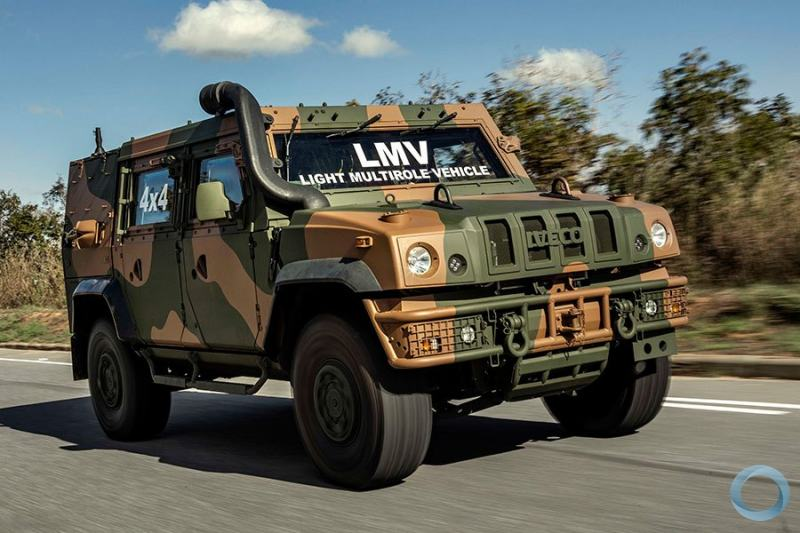
\includegraphics[width=0.7\linewidth]{images/lmv}
 	\fonte{http://www.defesanet.com.br/guarani/noticia/34800/VBMT-LSR---Exercito-Brasileiro-oficializa-a-compra-da-LMV--com-a-IVECO-Veiculos-de-Defesa-/}
 \end{figure} 
\vspace{10mm}

O exemplo mostra o balanço de forma reduzida, dado que existem relações complexas entre as camadas da sobrevivência. Em geral há forte envolvimento da massa do sistema na distribuição de quais camadas são ou não privilegiadas. Normalmente o aumento da capacidade de absorver impacto se dá por meio da inserção de placas massivas, diminuindo a mobilidade do sistema. Este trabalho tem foco na fundamentação da simulação de impacto balístico em veículos leves e coletes pessoais, portanto apenas projeteis pequenos com velocidade abaixo de $ 2000 m/s$ estão contemplados. \\

Para desenvolver este tipo de proteção é necessário entender como ela se comportará face aos impactos que irá sofrer. É possível fazer todo o estudo de comportamento e de possíveis melhorias usando apenas experimentação, porém esta não é a melhor opção em relação aos valores investidos. Um caminho viável para tal é usar simulações computacionais aliadas à experimentação. Este trabalho apresenta a fundamentação de uma ferramenta específica, a simulação computacional, aplicada em um contexto particular, que é o impacto projéteis consideravelmente pequenos em baixa velocidade. \\

As bases teóricas para a simulação computacional de um evento balístico são o foco desta revisão. A figura \ref{fig:diagramalog} mostra um diagrama com todos os maiores elementos da fundamentação teórica de uma simulação computacional de um impacto balístico. Nesta figura os retângulos são áreas abrangentes, enquanto os hexágonos são tópicos específicos da sua respectiva área abrangente. Cada área e seus tópicos serão revisados no trabalho, porém cabe aqui uma pequena introdução com intuito mostrar o posicionamento de cada área e a respectiva motivação de abordar tal assunto. \\

A contribuição da mecânica do contínuo é a definição das deformações finitesimais e das leis básicas do equilíbrio termodinâmico. Em um impacto balístico o projetil penetra o anteparo, gerando grandes deslocamentos e por conseguinte deformações. A deformação é um dado de entrada no modelo constitutivo, portanto descrever corretamente o tipo de deformação é muito importante em um evento balístico. O diagrama da figura \ref{fig:diagramalog} não mostra esta inserção para manter sua simplicidade e linearidade. Mesmo não estando evidente no diagrama a definição das deformações finitesimais é importante, já que este é um ponto de divergência entre o tipo de simulação mais comum na indústria, que usa deformações infinitesimais, e o tipo usado para simular um evento balístico. Sendo assim o primeiro passo dado no capítulo que aborda a mecânica do contínuo é a definição das deformações finitesimais. Os princípios termodinâmicos básicos limitam as possíveis configurações termodinâmicas da solução. A equação diferencial resolvida pelo método dos elementos finitos advém de um destes princípios, que é o balanço de momento linear. Portanto a definição dos princípios termodinâmicos básicos é a segunda etapa do capítulo que trata a mecânica do contínuo. \\

O método dos elementos finitos é abordado depois da mecânica do contínuo por ser usado para resolver o balanço de momento linear. A consideração de todos os fatores envolvidos em uma simulação de impacto balístico leva a um problema de alta complexidade, portanto não é interessante apresentar a fundamentação da ferramenta neste ambiente. A apresentação feita neste trabalho usa um problema simplificado, pois o objetivo é mostrar os constituintes básicos que por sua vez estão presentes desde o mais simples até o mais complexo dos problemas. \\

O comportamento dos materiais quando impactados é fundamentado pela plasticidade computacional, portanto este assunto é brevemente abordado para a posterior exposição dos modelos constitutivos mais usados na aplicação balística. O modelo constitutivo é acoplado ao método dos elementos finitos e é responsável por calcular o estado de tensão a depender de variáveis termodinâmicas da solução em um certo ponto e momento do tempo. Basicamente ele recebe variáveis termodinâmicas e devolve tensões, que por sua vez são usadas para resolver o equilíbrio mecânico, gerando um processo iterativo de resolução. \\

Por fim a mecânica da penetração é usada para definir o problema resolvido, por meio da geometria e das condições de contorno. Além disso a interpretação da simulação é feita com base nas teorias deste campo, por conseguinte é importante para um analista saber quais são, em teoria, os resultados possíveis da simulação. A mecânica do da penetração é um vasto campo, sendo assim o trabalho aborda a fundamentação teórica dos impactos em estruturas leves, com enfoque particular nos materiais cerâmicos. 

\begin{figure}[H]
 	\caption{\label{fig:diagramalog} Diagrama lógico da fundamentação teórica de uma simulação computacional de um impacto balístico}
 	\centering
 	\includegraphics[width=0.8\linewidth]{images/Diagrama Lógico TCC.png}
 	\fonte{O autor 2020}
 \end{figure} 
 


% ----------------------------------------------------------
\section{Objetivos}
% ----------------------------------------------------------

% ----------------------------------------------------------
\subsection{Objetivo Geral}
% ----------------------------------------------------------

Revisar a fundamentação teórica das áreas de maior influência na simulação computacional de um evento de impacto balístico.

% ----------------------------------------------------------
\subsection{Objetivos Específicos}
% ----------------------------------------------------------

\begin{itemize}
    \item Revisar os fundamentos da mecânica do contínuo com foco na descrição de deformações finitesimais e nas leis de equilíbrio.
    \item Revisar os fundamentos do método dos elementos finitos com foco em sistemas dinâmicos.
    \item Revisar os fundamentos da plasticidade computacional e apresentar os modelos constitutivos mais usados quando altas taxas de deformação estão presentes.
    \item Revisar o processo de penetração de projéteis com velocidades inferiores a $2000 m/s$, com enfoque em alvos feitos de material cerâmico.
\end{itemize}
% ---

% ---
% 2 - Desenvolvimento-
% ---
% ----------------------------------------------------------
\chapter{A Mecânica do contínuo} \label{Cap:MecCont}
% ----------------------------------------------------------

\section{Cinemática}
A cinemática é responsável pela descrição do movimento, mas desconsidera as forças envolvidas para gera-lo. A mecânica clássica descreve corpos como pontos no espaço. Sua descrição é limitada às quantidades cinemáticas deste único ponto, que normalmente é o centro de massa. De acordo com \cite{gurtin_fried_anand_2013} a propriedade básica de um corpo na mecânica do contínuo é que ele pode ocupar uma região do espaço euclideano. Além disso, de acordo com \cite{tadmor_miller_elliott_2012} a descrição do corpo não considera a estrutura que o constitui. Em um material descrito pela mecânica do contínuo importam apenas as propriedades macroscópicas, ou seja, propriedades verificadas em volume superior a um certo volume de controle. Neste viés, o seccionamento de qualquer corpo A, gerando os corpos B e C, faria com que as propriedades de B e C fossem iguais às de A.\par

Para \cite{hiermaier_2008} o corpo pode ser descrito como um acúmulo contínuo de pontos no espaço. Assim, dois pontos não podem ocupar o mesmo espaço, e um deles não pode ocupar mais de uma posição ao mesmo tempo. Para descrever pontos no espaço um sistema de coordenadas é necessário e o mais utilizado na mecânica do contínuo é o retangular cartesiano. No qual \ref{eq:kron} e \ref{eq:levi} são válidos. 
\begin{equation} \label{eq:kron}
    \boldsymbol{e_i \cdot e_j} = \gls{deltaK} = \left \{ \begin{array}{rcl}
       0  & \mbox{se} & i \neq j  \\
       1  & \mbox{se} & i = j
    \end{array} \right.
\end{equation}

Onde $ \gls{deltaK} $ é o símbolo de Kronecker Delta.

\begin{equation} \label{eq:levi}
    \boldsymbol{e_i \times e_j} = \gls{levicivita}\boldsymbol{e_k}
\end{equation}

Onde $ \gls{levicivita} $ é o Símbolo de Levi Civita. No qual 
\begin{equation}
    \gls{levicivita} = \left \{ \begin{array}{rcl}
       1  & \mbox{Para permutações pares de ijk.} & \mbox{ex: } 123  \\
       -1  & \mbox{Para permutações impares de ijk.} & \mbox{ex: } 132  \\
       0  & \mbox{se houver repetição nos índices.} 
    \end{array} \right.
\end{equation}

A mecânica do contínuo usa dois espaços para descrever um corpo. O primeiro é fictício e nele estão definidos os nomes das partículas do corpo. Considerando que o corpo pode ser descrito por um acúmulo contínuo de pontos, então nomear suas partículas usando pontos no espaço é conveniente. Assim sendo, o nome de cada partícula neste espaço é sua posição, logo o nome das partículas de um corpo é sua posição neste espaço. Por conta de ser usado para nomear as partículas, o primeiro espaço é chamado de espaço de referência. Nele reside a configuração do corpo chamada de material ou indeformada. Coordenadas referentes à esta configuração, portanto de seu correspondente espaço serão denotadas com letras maiúsculas ou com um subíndice $r$. \\

O segundo espaço é real, no sentido de que nele o corpo pode ser observado e medido. \cite{gurtin_fried_anand_2013} chama-o de espaço observado. Espacial ou deformada é a configuração do corpo no espaço chamado de real ou observado. Coordenadas referentes à configuração espacial serão denotadas com letra minúscula. Tensores serão sempre denotados por letras maiúsculas e negritadas, não importando a configuração a qual pertencem. \\

Usando estas configurações existem duas descrições mais utilizadas, vide figura \ref{fig:Euler_Lagrange}:
\begin{itemize}
    \item Descrição lagrangiana, material ou referencial: As variáveis independentes são $ \boldsymbol{X} $ e $ t$. O foco aqui é na partícula viajando no tempo. Esta é descrição a preferencial na mecânica dos sólidos, \cite{hiermaier_2008}.
    \item Euleriana ou espacial: As variáveis independentes são $ \boldsymbol{x} $ e $ t $. Nesta o foco está em uma posição do espaço, não importando qual partícula a assume em um determinado instante de tempo. Esta é a descrição preferencial na mecânica dos fluídos, \cite{hiermaier_2008}.
\end{itemize}

\begin{figure}[H]
    \centering
    \caption{Representação das diferentes descrições de um corpo.}
    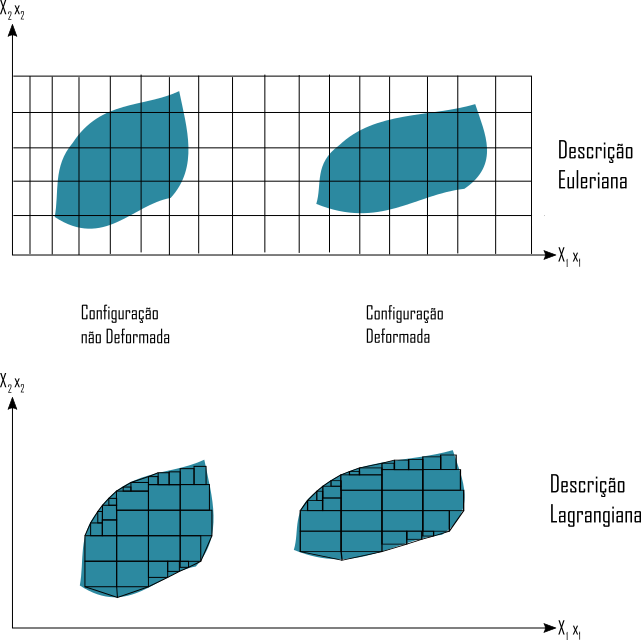
\includegraphics[width=0.8\linewidth]{images/EulervsLagrange.png}
    \label{fig:Euler_Lagrange}
    \fonte{O autor(2020)}
\end{figure}

%Figuras como a \ref{fig:Euler_Lagrange} podem ser vistas como inadequadas por especialistas na mecãnica do contínuo, já que representam no mesmo sistema as coordenadas de referência e espaciais. É necessário explicitar que os dois, embora sejam espaços euclideanos, são diferentes. A representação na figura se vale de um caso particular muito comum em que a configuração de referência e a espacial estão descritas com os mesmos vetores de base e são coincidentes em $ t=0 $. Além disso a figura \ref{fig:Euler_Lagrange} apela para a existência de uma malha, inserida no contexto do método dos elementos finitos, para representar a diferença entre as descrições, porém o método os elementos finitos nada mais é do que uma ferramenta para resolver as equações de equilíbrio. As descrições Lagrangianas e Eulerianas são indepentes do método de solução. \par

Dado que um corpo contínuo pode ser visto como uma aglomeração de pontos no espaço, então o movimento de uma partícula pode ser representado pelo vetor deslocamento. Este vetor em sua descrição lagrangiana é calculado pela expressão \ref{eq:desl_lag}, que em sua descrição euleriana corresponde à \ref{eq:desl_euler}.
\begin{align}
&\boldsymbol{U}(\boldsymbol{X},t) = \mathcal{X}(\boldsymbol{X},t) - \boldsymbol{X}
\label{eq:desl_lag}\\
&\boldsymbol{u}(\boldsymbol{x},t) = \boldsymbol{x} - \mathcal{X}^{-1}(\boldsymbol{x},t)
\label{eq:desl_euler}
\end{align}

Onde a função $ \mathcal{X} $, tal que $ \boldsymbol{x} = \mathcal{X}(\boldsymbol{X},t) $, chama-se função movimento e é responsável por mapear a localização de uma partícula em um determinado tempo. Observa-se que $ \boldsymbol{u}(\boldsymbol{x},t) =  \boldsymbol{U}(\boldsymbol{X},t)  $, já que ambos representam o mesmo campo de deslocamentos, porém descrito de formas diferentes. \par

Possuindo os deslocamentos é possível descrever as deformações provenientes destes deslocamentos.\footnote{É importante notar que há um acumulo de termos quando se trata da mecânica do contínuo em português. O atual assunto é traduzido como deformação, porém em inglês trata-se de "deformation". O conceito da deformação usual, que é causadora de tensões, será abordado nas próximas seções e em inglês chama-se "strain". Por hora a diferença não é pronunciada, porém no futuro ela será novamente citada.} O campo primordial quando o assunto é a descrição das deformações chama-se gradiente da deformação $ \boldsymbol{F} $, eq. \ref{eq:desl_grad}.
% CONTINUAR REVISÃO %
\begin{align}\label{eq:desl_grad}
    \boldsymbol{F}(\boldsymbol{X},t) = \boldsymbol{F} \\
    F_{ij} = \frac{\partial \mathcal{X}_i}{\partial X_j}
\end{align}

São duas as possíveis formas de deformação em um corpo, a forma homogênea e a não homogênea. Basicamente as deformações homogêneas são aquelas onde o gradiente da deformação é independe da posição no corpo. De forma geral pode se dizer que sendo $ \boldsymbol{dx} $ uma fibra espacial infinitesimal e $ \boldsymbol{dX} $ uma fibra material infinitesimal. Tanto para deformações homogêneas quanto para não homogêneas é válida a eq. \ref{eq:nonhomdef}. Esta equação mostra que as fibras infinitesimais deformadas são resultado de uma transformação das fibras deformadas, esta transformação é caracterizada pelo tensor $\boldsymbol{F}$.

\begin{equation}
    \boldsymbol{dx} = \boldsymbol{F}(\boldsymbol{X},t) \boldsymbol{dX}
    \label{eq:nonhomdef}
\end{equation}


%O determinante do gradiente da deformação é chamado por \cite{gurtin_fried_anand_2013} de Jacobiano volumétrico e por \cite{hiermaier_2008} de determinante do Jacobiano. Doravante este determinante será chamado de jacobiano ou $ J $. Esta simplificação ocorrerá pois o jacobiano de área não será abordado.
%\begin{equation}
%    J = det(\boldsymbol{F}) = \frac{dv}{dV}
%\end{equation}

O tensor $\boldsymbol{F}$ caracteriza uma transformação das fibras de indeformadas para deformadas. Esta descrição leva em consideração tanto a rotação quanto o estiramento das fibras. Para separar estas é usado um teorema chamado de decomposição polar, apresentado aqui sem prova. \footnote{A prova encontra-se em \cite{gurtin_fried_anand_2013} pg.33}

\begin{equation}
    \boldsymbol F = \boldsymbol{RU} = \boldsymbol{VR}
\end{equation}

Esta é uma decomposição multiplicativa, na qual, o tensor de deformações $ \boldsymbol{F} $ é separado em uma parte relacionada à rotação de corpo rígido e uma ao estiramento do corpo. São elas respectivamente $ \boldsymbol{R} $ e $ \boldsymbol{U} $ ou $ \boldsymbol{V} $, onde $ \boldsymbol{\gls{R}}$ é um tensor ortogonal. $ \boldsymbol U = \boldsymbol{U}(\boldsymbol{X},t) $ é chamado de tensor de estiramento direito e pertence à configuração material. Já $ \boldsymbol V = \boldsymbol{V}(\boldsymbol{x},t) $ chama-se tensor de estiramento esquerdo e pertence à configuração espacial, de acordo com \cite{intromec}. Usando $ \boldsymbol{\gls{V}} $  e $ \boldsymbol{\gls{U}} $ é possível chegar a outros dois tensores, são eles $ \gls{C}$ e \gls{B}. $ \boldsymbol{\gls{C}} $ é o tensor deformação direito de Cauchy-Green e $ \boldsymbol{\gls{B}} $ é o tensor deformação esquerdo de Cauchy-Green. 

\begin{align}
    & \boldsymbol{C} = \boldsymbol{F^TF} = \boldsymbol{U}^2 \\
    & \boldsymbol{B} = \boldsymbol{FF^T} = \boldsymbol{V}^2
\end{align}

Conhecendo $\boldsymbol{C}$ é possível introduzir a deformação da forma mais conhecida na engenharia, que é a traduzida da palavra em inglês "strain". O tensor deformação de Green-Lagrange $ \boldsymbol{E} $ representado na equação \ref{eq:green_lag} é um tensor finitesimal de deformação, por conta disso é adequado para medir deformações arbitrariamente grandes.

\begin{equation}
   \boldsymbol{E}(\boldsymbol{X},t) =  \boldsymbol{E} = \frac{1}{2}(\boldsymbol{F^TF - I}) = \frac{1}{2}(\boldsymbol{C - I}) = \frac{1}{2}(\boldsymbol{U^2 - I})
    \label{eq:green_lag}
\end{equation}

 O tensor de Green-Lagrange pode ser escrito de forma diferente, em função do gradiente dos deslocamentos. Para tal, é apresentado o tensor $\boldsymbol{H}$, que é o gradiente do deslocamento.
\begin{equation}
    \boldsymbol{H} = \nabla \boldsymbol{u}
    \label{eq:desl_gradH}
\end{equation}
O tensor $ \boldsymbol{H} $ se relaciona com $ \boldsymbol{F} $ da seguinte forma:

\begin{equation}
    \boldsymbol{F} = \boldsymbol{I + H}
\end{equation}

Onde $ I $ é o tensor identidade.
Ao inserir a relação entre $\boldsymbol{\gls{F}} $ e $ \boldsymbol{\gls{H}} $ no tensor de Green-Lagrange, este pode ser escrito em função do gradiente do deslocamento. 

 \boldmath\begin{align}
    E &= \frac{1}{2}((I + H)^T(I+H) - I)\\
    &=\frac{1}{2}((I + H^T)(I+H)-I) \\
    &= \frac{1}{2}(I + H + H^T + H^TH - I )\\
    &= \frac{1}{2}(H + H^T + H^TH) \\
    &= \frac{1}{2}(\nabla u + \nabla u^T + \nabla u^T\nabla u)
    \label{eq:green_lag_desl}
\end{align} \unboldmath

O tensor deformação de Green-Lagrange escrito em função do gradiente do deslocamento é o ponto de partida para a dedução de um tensor chamado deformação infinitesimal,  $ \boldsymbol{\gls{eps}} $. Este tensor é uma linearização da deformação de Green-Lagrange. Sendo assim, ele é válido, apenas, para deformações de ordem infinitesimal, já que desconsidera o termo de maior ordem do tensor $ \gls{E} $. Sua expressão é dada a seguir.

\begin{equation} \label{eq:definfi}
    \boldsymbol{\varepsilon} = \frac{1}{2}(\nabla \boldsymbol{u} + \nabla \boldsymbol{u}^T)
\end{equation}

Para ilustrar o comportamento dos tensores de deformação $\boldsymbol{E}$ e $\boldsymbol{\varepsilon}$ a seguinte função movimento é aplicada a um cubo de dimensões unitárias. 
\begin{align}
	x_1 &= X_1 + tX_1 \\
	x_2 &= X_2 \\
	x_3 &= X_3 
\end{align}

Este movimento denota um estado uniaxial de deformação fictício. Note que no instante $t=1$ o corpo já tem um aumento de 100\% de seu comprimento. Deformação na casa dos $100\%$ não são comuns em situações estáticas, porém o mesmo não pode ser dito em um impacto balístico. Em simulações de impactos balísticos é comum obter deformações na casa dos $ 200\% $ ou mais. Tais deformações não são numericamente interessantes, então um recurso chamado erosão entra em ação. Na erosão o elemento é deletado quando alguma variável limitadora atinge certo valor. Na literatura o uso da deformação como variável limitadora é dominante, o valor padrão para a deformação que ativa a erosão é 150\%, vide \cite{theorymanls}.  \par

\begin{figure}[H]
\caption{Participação das parcelas do tensor de Euler-Lagrange}
\centering
	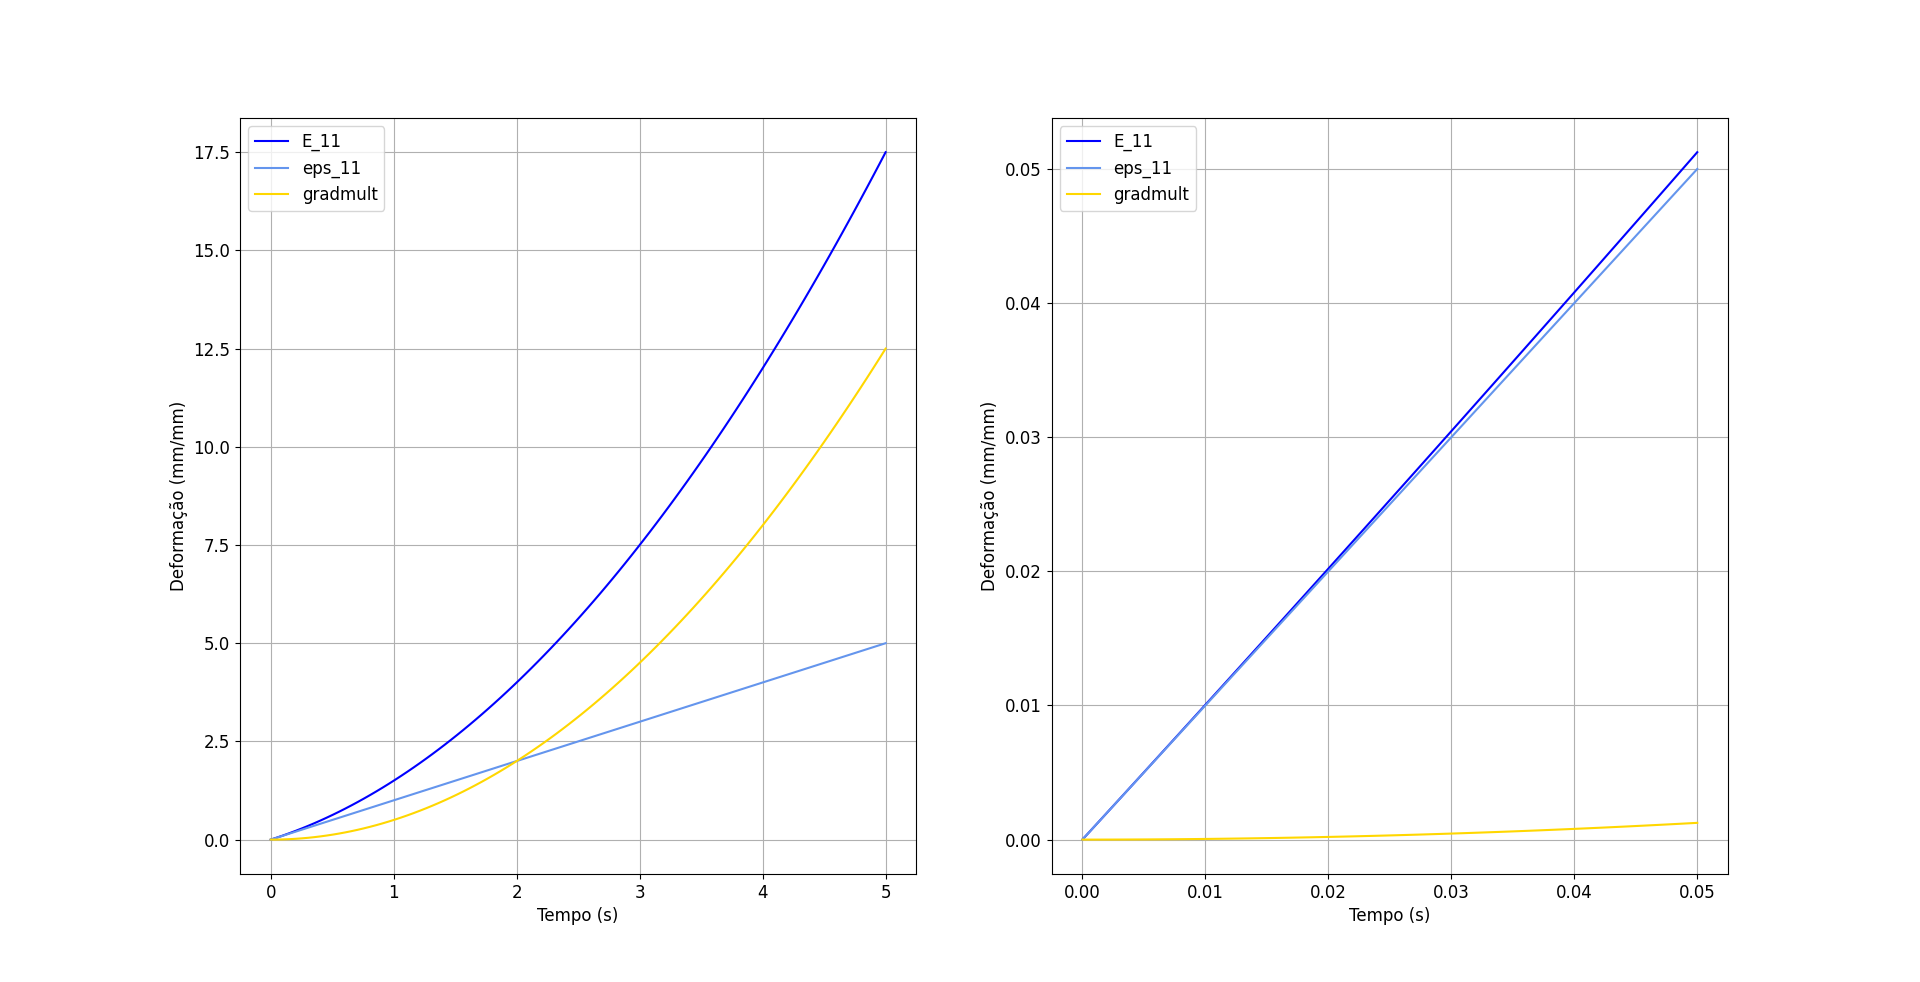
\includegraphics[width = \textwidth]{images/quest3ex.png}
	\label{fig:gradmult}
	\fonte{O autor (2020)}
\end{figure}

A figura \ref{fig:gradmult} denota a componente 11 das matrizes que representam o tensor de Green-Lagrange e o de deformações infinitesimais para um corpo submetido ao movimento supracitado. Observa-se que, em baixos níveis de deformação, imagem a direita, a parcela de maior ordem, gradmult, permanece com valor irrisório. Neste caso os valores do tensor de Green-Lagrange e o de deformações infinitesimais são semelhantes. Dado que computacionalmente o tensor infinitesimal tem custo menor, ele é usado na grande maioria dos casos. A deformação infinitesimal apenas se aplica aos casos nos quais as deformações e os deslocamentos são muito pequenos. A motivação para tal é que a partir de certo ponto a parcela chamada de gradmult começa a ter influência significativa no tensor $ \gls{E} $, fazendo com que $ \gls{E} $ e $ \gls{eps} $ se distanciem. \par

Além dos tensores $ \gls{E} $ e $ \boldsymbol{\gls{eps}} $ existem outros que são muito usados para medir a deformação em um corpo contínuo, porém $\gls{E}$ é o mais relevante e os outros não serão abordados para manter a brevidade do trabalho. \\

Como este trabalho trata apenas dos fundamentos, as deformações infinitesimais serão usadas para abordar os conteúdos que seguem. Porém, em uma aplicação real seria necessário adaptar tais formulações às deformações finitesimais.

\section{Princípios termomecânicos básicos}

\subsection{O balanço de massa}

A conservação de massa em sua forma global é apresentada na equação \ref{eq:consmassa}

\begin{equation}
    \int_{\Omega_r} \rho_r(\boldsymbol{X}) dV(\boldsymbol{X}) = \int_{\Omega} \rho(\boldsymbol{x},t) dv(\boldsymbol{x}) 
    \label{eq:consmassa}
\end{equation}

Onde $ \gls{Omegar} $ e $ \gls{Omega} $ são, respectivamente, a região ocupada pelo corpo na configuração material e espacial. Já $ \gls{rhor} $ e $ \gls{rho} $ são, respectivamente, a densidade do corpo na configuração material e espacial. Como o braço esquerdo da equação \ref{eq:consmassa} não depende do tempo, ao deriva-la o resultado é a equação \ref{eq:consmassa2}. O símbolo $ \dot{\overline{entidade}} $ significa a derivação no tempo da entidade em questão.
\begin{equation}
    \dot{\overline{\int_{\Omega} \rho(\boldsymbol{x,t}) dv(\boldsymbol{x})}} = 0
    \label{eq:consmassa2}
\end{equation}

O teorema do transporte de Reynold é aplicado na equação \ref{eq:consmassa2} tendo \ref{eq:consmassalocal0} como resultado. Admitindo que cada subdivisão do corpo deve respeitar a eq. \ref{eq:consmassalocal0}, a forma local do balanço de massa, eq \ref{eq:consmassalocal}, é alcançada.\footnote{O teorema do transporte de Reynold pode ser encontrado em \cite{gurtin_fried_anand_2013} pg. 113}

\begin{align}
    \int_{\Omega} (\dot{\rho} + \rho div\boldsymbol{v})  dv &= 0 \label{eq:consmassalocal0} \\
    \dot{\rho} + \rho \; div\boldsymbol{v} &= 0 \label{eq:consmassalocal}
\end{align}

O balanço de massa deve ser respeitado tanto na formulação lagrangiana quanto na euleriana. Porém, na formulação euleriana o balanço de massa se torna mais difícil de obedecer, já que pode haver fluxo do material através da malha. Este fluxo deve ser calculado e levado em consideração durante uma simulação. Quando se trata de uma descrição lagrangiana não há fluxo de material entre os elementos, sendo assim obedecer a conservação de massa se torna mais fácil. 

\subsection{Balanço de momento linear e angular}

Um ponto importante para a discussão a seguir é assumir que o observador dos fenômenos está inerte. \par

Primeiro é definido um vetor $ \boldsymbol{r(x) = x - 0} $ que reside na configuração espacial, onde $ \boldsymbol{o} $ é a origem. São apresentados nas equações \ref{eq:linmoment} e \ref{eq:angmoment} o momento linear e angular respectivamente.

\begin{align}
    \boldsymbol{l}(\Omega) = \int_{\Omega} \rho \boldsymbol{v} dv \label{eq:linmoment} \\
    \boldsymbol{a}(\Omega) = \int_{\Omega} \boldsymbol{r} \times \rho \boldsymbol{v} dv \label{eq:angmoment}
\end{align}

Como uma consequência do balanço de massa, de acordo com \cite{gurtin_fried_anand_2013}, é possível escrever a derivada temporal do momento linear e angular da seguinte forma.

\begin{align}
   \dot{\overline{\boldsymbol{l}(\Omega)}} = \int_{\Omega} \rho \dot{\boldsymbol{v}} dv \label{eq:linmoment} \\
   \dot{\overline{\boldsymbol{a}(\Omega)}} = \int_{\Omega} \boldsymbol{r} \times \rho \dot{\boldsymbol{v}} dv \label{eq:angmoment}
\end{align}

Para completar a descrição do balanço, falta discutir a aplicação de força em um corpo. \cite{gurtin_fried_anand_2013} afirma que existem três tipos de força na mecânica do contínuo. 
\begin{itemize}
    \item Forças de contato entre regiões adjacentes, que tem interseção ao longo de seu contorno.
    \item Forças de contato no contorno do corpo, que são exercidas pelo ambiente.
    \item Forças de corpo em todos os pontos, que são exercidas pelo ambiente em todos os pontos do corpo.
\end{itemize}
De acordo com \cite{gurtin_fried_anand_2013} um dos maiores axiomas da mecânica do contínuo é a hipótese de Cauchy. Ela refere-se às forças de contato e está representada graficamente na figura \ref{fig:hipotesecauchy}. 

\begin{figure}[H]
    \centering
    \caption{Representação gráfica da hipótese de Cauchy}
    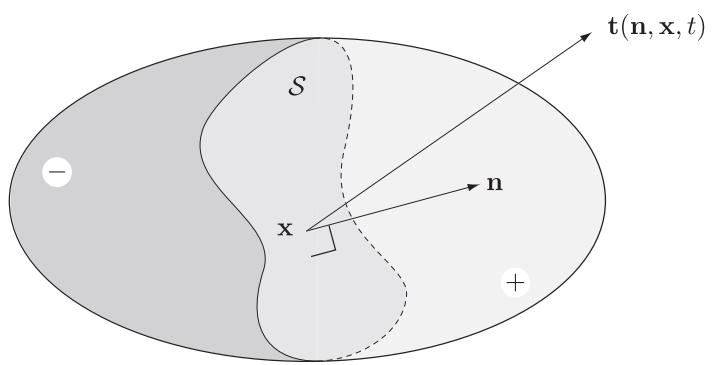
\includegraphics[width = 0.7 \textwidth]{images/hipoteseCauchy.png}
    \label{fig:hipotesecauchy}
    \fonte{\cite{gurtin_fried_anand_2013}}
\end{figure}

Em sua hipótese, Cauchy insere um campo de tração superficial, $ \boldsymbol{t}(\boldsymbol{x, n},t) $, definido para cada vetor normal unitário $ \boldsymbol{n} $, ponto $ \boldsymbol{x} $ pertencente ao corpo e tempo $ t $. O campo $ \boldsymbol{t}(\boldsymbol{x, n},t) $ tem a seguinte propriedade: Dada qualquer superfície espacial $ S $ pertencente ao corpo, $ \boldsymbol{t}(\boldsymbol{x, n},t) $ representa a força por unidade de área exercida através de $ S $. De acordo com a figura \ref{fig:hipotesecauchy} a superfície divide o corpo em duas porções. A porção negativa, localizada à esquerda de $S$, e a porção positiva, localizada à direita. A força exercida através de $S$, de acordo com \cite{gurtin_fried_anand_2013}, é aplicada no material, na porção negativa, e pelo material, na porção positiva.  \\

De acordo com \cite{gurtin_fried_anand_2013} para descobrir a força entre regiões adjacentes $ P $ e $D$ é necessário  integrar a tração ao longo da superfície $ S=P\cap D $. O resultado desta é a expressão \ref{eq:forçasup}.

\begin{equation}
    \int_{S} \boldsymbol{t(n)}\, da = \int_{S} \boldsymbol{t}(\boldsymbol{x, n},t) \, da(\boldsymbol{x})
    \label{eq:forçasup}
\end{equation}

Portanto, ao considerar toda a superfície do corpo, a região $S$ passa a ser escrita como $\partial \Omega$. A força total exercida pelo meio no corpo $ \Omega $ é descrita pela expressão \ref{eq:forçasuptot}. Onde $\boldsymbol{n}$ é a normal da superfície do corpo no ponto no qual $\boldsymbol{t}$ está sendo avaliado e $\partial \Omega$ é toda a superfície do corpo.
\begin{equation}
    \int_{\partial \Omega} \boldsymbol{t(n)} \, da
    \label{eq:forçasuptot}
\end{equation}

O meio também pode exercer força ao longo de todo o volume do corpo. Um exemplo clássico é a força gravitacional. Esse tipo de força é descrita pela expressão \ref{eq:forçavoltot}.

\begin{equation}
    \int_{\Omega} \boldsymbol{b} \, dv
    \label{eq:forçavoltot}
\end{equation}

Conhecendo  $\gls{t}$ e $\gls{b}$ é possível definir a força e o momento líquidos em $ \gls{Omega}$, respectivamente expressões \ref{eq:forçaliq} e \ref{eq:momliq}.

\begin{align}
    \boldsymbol{f}(\Omega) = \int_{\partial \Omega} \boldsymbol{t(n)} \, da + \int_{\Omega} \boldsymbol{b} \, dv \label{eq:forçaliq} \\
    \boldsymbol{m}(\Omega) = \int_{\Omega} \boldsymbol{r} \times \boldsymbol{t(n)} \, da + \int_{\Omega} \boldsymbol{r} \times \boldsymbol{b} \, dv \label{eq:momliq}
\end{align}

A igualdade entre a derivada temporal do momento linear e a força total exercida no corpo expressa o balanço de momento linear, apresentado na expressão \ref{eq:linbal}. De maneira semelhante, a igualdade entre a derivada temporal do momento angular e o momento líquido exercido no corpo expressa o balanço de momento angular, apresentado na expressão \ref{eq:angbal}.

\begin{equation}
    \int_{\partial \Omega} \boldsymbol{t(n)} da + \int_{\Omega} \boldsymbol{b} dv = \int_{\Omega} \rho \dot{\boldsymbol{v}} dv \label{eq:linbal} 
\end{equation}

\begin{equation}
    \int_{\partial \Omega} \boldsymbol{r} \times \boldsymbol{t(n)} da + \int_{\Omega}    \boldsymbol{r} \times \boldsymbol{b} dv = \int_{\Omega} \boldsymbol{r} \times \rho \dot{\boldsymbol{v}} dv \label{eq:angbal} 
\end{equation}

O teorema de Cauchy é apresentado, sem prova-lo.\footnote{A prova do teorema de Cauchy pode ser encontrada em \cite{gurtin_fried_anand_2013} pg. 137}. De acordo com o teorema, uma consequência do balanço de momento linear é que existe um tensor $\gls{Cauchy}$ chamado tensor de tensões de Cauchy. Tal que a expressão \ref{eq:CauchyStress} é válida.

\begin{equation}
    \boldsymbol{t(n)} = \boldsymbol{\sigma n} \label{eq:CauchyStress}
\end{equation}

O teorema de Cauchy possibilita derivar a forma local tanto do balanço de momento linear quanto do balanço de momento angular. A derivação do balanço de momento linear local será feita a seguir. Porém, a derivação do balanço de momento angular local não será feita, por conta de sua extensão. Esta pode ser encontrada em \cite{gurtin_fried_anand_2013} pg. 140 e resulta que $ \gls{Cauchy} = \gls{Cauchy}^T $, portanto o balanço de momento angular local implica a simetria do tensor de tensões de Cauchy. \par

O ponto de partida é o balanço de momento linear global, eq. \ref{eq:linbal}. O teorema de Cauchy é aplicado chega-se na eq. \ref{eq:forma2}. Ao aplicar o teorema do divergente no primeiro termo do braço esquerdo da eq. \ref{forma2}, a expressão \ref{eq:forma3} é obtida.\footnote{ O teorema do divergente implica na igualdade entre uma integral ao longo de um contorno e uma integral no volume deste contorno. Uma explicação deste pode ser encontrada em \cite{gurtin_fried_anand_2013} pg. 52. } De acordo com \cite{gurtin_fried_anand_2013} a expressão \ref{eq:forma3} é válida para qualquer subdivisão do corpo. Isto possibilita assumir que para qualquer ponto a eq. \ref{eq:locallinbal} deve ser atendida. O nome dado à expressão \ref{eq:locallinbal} é forma local do balanço de momento linear na configuração espacial. 
\begin{align}
    &\int_{\partial \Omega} \boldsymbol{t(n)} \, da + \int_{\Omega} \boldsymbol{b}\, dv = \int_{\Omega} \rho \dot{\boldsymbol{v}} \,dv \\
    &\int_{\partial \Omega} \boldsymbol{\sigma n} \,da + \int_{\Omega} \boldsymbol{b}\, dv = \int_{\Omega} \rho \dot{\boldsymbol{v}} \,dv \label{eq:forma2} \\ 
    &\int_{\Omega} \boldsymbol{div \sigma} \,dv + \int_{\Omega} \boldsymbol{b} \,dv = \int_{\Omega} \rho \dot{\boldsymbol{v}} \,dv  \label{eq:forma3} \\
    &div\gls{Cauchy} + \boldsymbol{b} = \rho \boldsymbol{\dot{v}} \label{eq:locallinbal}
\end{align}
%TODO O RESTO ESTÁ COMENTADO
\begin{comment}
\subsection{Balanço de potencias}

A equação \ref{eq:locallinbal}, o balanço local do momento linear, foi apresentada na configuração espacial. O balanço de potencias será trabalhado na configuração material e por conta disso é apresentada a equação \ref{eq:locallinbalmat}, que é o balanço de momento linear local na configuração material. Houve uma pequena alteração na notação usada até agora, na expressão \ref{eq:locallinbalmat} as quantidades relacionadas à configuração material não estão mais maiúsculas e sim com um $r$ subscrito. Além disso é inserido o primeiro tensor tensão de Piola-Kirchhoff $\gls{P}$, que pertence à configuração material. Ele é chamado de tensão de engenharia em uma curva tensão deformação de engenharia, enquanto o tensor tensão de Cauchy é a tensão real. 

\begin{equation} \label{eq:locallinbalmat}
    Div\gls{P} + \boldsymbol{b}_r = \rho_r \ddot{\mathcal{X}}
\end{equation}

É necessário apontar que $ div \boldsymbol{A} \neq Div \boldsymbol{A} $, dado que $ div \boldsymbol{A} = \frac{\partial A_{ij}}{\partial x_j} $ e $ Div \boldsymbol{A} = \frac{\partial A_{ij}}{\partial X_j} $, usando novamente a notação onde $ \boldsymbol{X = x_r}$. A transição do balanço de momento linear de local para global faz com que a equação \ref{eq:locallinbalmat} tenha a seguinte forma.

\begin{equation}
    \int_{\partial \Omega_r} \boldsymbol{Pn}\, da_r + \int_{\Omega_r} \boldsymbol{b}_r \,dv_r = \int_{\Omega} \rho_r \ddot{\mathcal{X}}\, dv_r
    \label{eq:globallinmat}
\end{equation}

O primeiro passo para chegar na expressão do balanço de potencias é fazer um produto interno à direita em \ref{eq:globallinmat} com a velocidade $ \dot{\mathcal{X}} $, gerando \ref{eq:globallinmat2}.

\begin{equation}
    \int_{\partial \Omega_r} \boldsymbol{Pn} \cdot \dot{\mathcal{X}} \, da_r + \int_{\Omega_r} \boldsymbol{b}_r \cdot \dot{\mathcal{X}} \,dv_r = \int_{\Omega} \rho_r  \ddot{\mathcal{X}} \cdot \dot{\mathcal{X}} \,dv_r
    \label{eq:globallinmat2}
\end{equation}

O braço direito da equação acima é equivalente à taxa de variação da energia cinética, de acordo com \ref{eq:cineneqv}.\footnote{Basta derivar o braço direito usando a regra da multiplicação para chegar no braço esquerdo.}

\begin{equation} \label{eq:cineneqv}
    \int_{\Omega} \rho_r  \ddot{\mathcal{X}} \cdot \dot{\mathcal{X}} dv_r = \frac{d}{dt} \int_{\Omega_r} \frac{1}{2}\rho_r |\dot{\mathcal{X}}|^2 dv_r= \dot{\overline{\mathcal{K}(\Omega_r)}}
\end{equation}

O foco agora é o primeiro termo do braço direito da equação \ref{eq:globallinmat2}. Ao aplicar o teorema do divergente a este termo a seguinte expressão é atingida.\footnote{Tal identidade é apresentada na pg. 56 de \cite{gurtin_fried_anand_2013}}

\begin{equation}
    \int_{\partial \Omega_r} \boldsymbol{Pn} \cdot \dot{\mathcal{X}} \,da_r = \int_{\Omega} (\dot{\mathcal{X}} \cdot Div\boldsymbol{P} + \boldsymbol{P} : \dot{\boldsymbol{F}} )\,dv_r
    \label{eq:transpowerbalance}
\end{equation}

Perceba que no primeiro termo dentro da integral no braço direito de  \ref{eq:transpowerbalance} é possível aplicar o balanço de momento linear da forma local, $ Div \boldsymbol{P} = \rho_r \ddot{\mathcal{X}} - \boldsymbol{b}_r $, obtendo o balanço de potências na configuração material. 

\begin{equation} \label{eq:baldepotencias}
     \underbrace{\int_{\partial \Omega_r} \gls{P}\boldsymbol{n}_r \cdot \dot{\mathcal{X}} \,da_r + \int_{\Omega_r} \boldsymbol{b}_r \cdot \dot{\mathcal{X}} \,dv_r}_\text{Potência externa $\gls{convpower}$ } = \underbrace{\int_{\Omega_r} \boldsymbol{P}: \dot{\boldsymbol{F}} \,dv_r}_\text{Potência interna $\gls{Pint}$ } + \underbrace{\frac{d}{dt} \int_{\Omega_r} \frac{1}{2}\rho_r |\dot{\mathcal{X}}|^2 \,dv_r}_\text{Variação da energia cinética $\dot{\mathcal{K}}_(\Omega_r)$} 
\end{equation}

\subsection{Balanço de energia}

O balanço de energia ou a primeira lei da termodinâmica quando aplicado ao contínuo toma, em sua forma global, a forma apresentada na expressão \ref{eq:primeiralei}. Nele o termo $ \gls{e_r} $ denota a energia interna do corpo na configuração material. O vetor $\boldsymbol{q}_r$ é o fluxo de calor para o corpo e $q_r$ é um escalar que representa fluxos de calor irradiados.

\begin{align}  \label{eq:primeiralei}
  \int_{\Omega_r} (\dot{e_r} + \frac{1}{2} \rho_r|\ddot{\mathcal{X}}|^2) dv_r = -&\int_{\partial \Omega_r} \boldsymbol{q}_r \cdot \boldsymbol{n}_r da_r + \int_{\Omega} q_r dv_r + \\ \notag 
    &\int_{\partial \Omega_r} \boldsymbol{Pn_r} \cdot \dot{\mathcal{X}} da_r + \int_{\Omega} \boldsymbol{b}_r \cdot \dot{\mathcal{X}} dv_r
\end{align}

Usando o balanço de potencias \ref{eq:baldepotencias} chega-se na forma do balanço de energia mais utilizada em códigos de propagação de ondas.\footnote{Este é um nome alternativo ao jargão que vem do inglês Hydrocode.} Nesta forma $\dot{\gls{Etot}}$ é a derivada no tempo da energia total do corpo.

\begin{equation} \label{eq:balenergia}
    \underbrace{\int_{\Omega_r} \dot{e_r} dv_r}_\text{$\dot{\mathcal{E}}_{tot}(\Omega_r)$} = \underbrace{\int_{\partial \Omega_r} \gls{P}\boldsymbol{n}_r \cdot \dot{\mathcal{X}} da_r + \int_{\Omega_r} \boldsymbol{b}_r \cdot \dot{\mathcal{X}} dv_r}_\text{$\gls{convpower}$ } \underbrace{-\int_{\partial \Omega_r} \boldsymbol{q}_r \cdot \boldsymbol{n}_r da_r + \int_{\Omega} q_r dv_r}_\text{Fluxo de calor $ \gls{Q} $}
\end{equation}

A equação \ref{eq:balenergia} termina a descrição dos princípios termo-mecânicos básicos. A segunda lei da termodinâmica não foi citada por ter maior representação como uma limitação à teoria constitutiva dos materiais, elas é usada para cunhar modelos consistentes. A teoria constitutiva não será abordada em termos de suas das limitações e teorias energéticas envolvidas, no entanto os modelos constitutivos serão apresentados e discutidos de forma expositiva.

\end{comment}



\chapter{O método dos elementos finitos}

\section{Introdução}
O método dos elementos finitos auxiliou muitos dos maiores desenvolvimentos industriais nos últimos anos e sua expansão está, em boa quantia, ligada ao avanço dos computadores modernos. Sua flexilidade e versatilidade são potencializadores de seu recente domínio no campo das análises computacionais. O método foi criado para a aplicação na mecânica dos sólidos, porém hoje é usado em aplicações diversas. Este trabalho está inserido na área originaria do método, por conseguinte a explicação será de forma canônica, desconsiderando as aplicações que fogem do escopo geral da mecânica dos sólidos. \\

\begin{comment}
"The limitations of the human mind are such that it cannot grasp the behavior of its
complex surroundings and creations in one operation." \cite{zienkiewicz2013}. \\

Os limites da mente humana são tais que ela não pode compreender o comportamento de seus complexos arredores e criações em uma única operação. Esta frase quer dizer que nem sequer entendemos nosso meio em apenas uma iteração, portanto não é esperado que consigamos replicar tais comportamentos em apenas uma iteração. 
\end{comment}
A divisão de tarefas complexas é uma prática comum em todos os campos do conhecimento. A linha de produção de automóveis exemplifica um processo complexo extremamente segmentado .\\ Um problema discreto é caracterizado por ser subdividido em porções finitas que compõe um inteiro bem definido. De acordo com \cite{zienkiewicz2013} este é o único tipo de problema que pode ser resolvidos por um computador. O ato de escrever um programa, que nada mais é do que uma lista de instruções a ser seguida, perpassa pela descrição do problema em pacotes de tamanho administrável. \\

Porém de acordo com \cite{zienkiewicz2013}, a formulação física e matemática da maioria dos problemas, que valem a pena ser resolvidos, forma um sistema contínuo que por sua vez é composto por porções ditas infinitesimais. Estes componentes são tão pequenos quanto devaneios permitirem, portanto formam um problema de dimensão infinita. Resolver um problema contínuo, é impossível a um computador, dado que isto implicaria seguir uma sequência infinita de instruções até o fim do problema. \\ 

A solução de sistemas contínuos faz uso de conceitos e manipulações matemáticas que levam à solução exata do problema, porém este tipo de solução infelizmente está limitada aos problemas de menor complexidade que não por isso são de menor importância. De acordo com \cite{zienkiewicz2013} para resolver problemas de maior complexidade são necessárias técnicas de discretização. Tais técnicas são responsáveis pela transformação de problemas contínuos em discretos. A consequência desta transformação é que a outrora solução exata torna-se uma aproximação. \\

A técnica de discretização mais usada no âmbito da mecânica dos sólidos é a dos elementos finitos. De acordo com \cite{zienkiewicz2013} não há uma data exata para especificar o dia e ano de sua criação. Porém, um dos primeiros artigos,  que usa o nome: Método dos Elementos Finitos, foi escrito por Ray Willian Clough em 1960, \cite{CloughFEA}. Muito embora Clough tenha sido um dos primeiros a dar nome ao método, ele não foi um dos primeiros a fazer contribuições significativas. Neste grupo estão: Lord Rayleigh, \cite{Rayleigh}, como um dos primeiros participantes falando sobre métodos variacionais. Boris Grigoryevich Galerkin,\cite{Galerkin}, criador do método de Galerkin e possivelmente um dos maiores contribuintes históricos para o método dos elementos finitos. A última grande contribuição vem do que provavelmente pode ser chamado de método irmão, que é o das diferenças finitas. \footnote{Algumas outras contribuições foram decisivas para se chegar no estado atual, porém  para uma leitura mais detalhada da criação do método cita-se ,\cite{zienkiewicz2013} Pg. 1-4, como uma fonte concisa e rápida da sua criação.} \\

Neste trabalho a técnica dos elementos finitos será apresentada sem considerar qualquer não linearidade. Não linearidades podem ser relacionadas ao material, quando um modelo não elástico é usado, à geometria, quando há contato ou grandes deslocamentos e/ou deformações e às cargas, quando são seguidoras. Esta apresentação simplificada é justificada pelo compartilhamento das bases formadoras do método em problemas lineares e não lineares.  \\

Em problemas envolvendo impacto balístico as não linearidades encontradas são relacionadas ao material e à geometria. No material a ocorrência de deformações plásticas insere a necessidade de modelos constitutivos não lineares. Quanto à geometria, grandes deslocamentos e deformações estão presentes neste tipo de evento, portanto há necessidade de usar o tensor de deformações finitesimais para sua descrição. \\ 

Como dito anteriormente as não linearidades serãoo desconsideradas, portanto as deformações serão consideradas infinitesimais. Além disso, os efeitos da temperatura não serão levados em consideração. Como apresentado no \ref{Cap:MecCont} a expressão \ref{eq:locallinbal} é a forma local do balanço de momento linear, também chamada de primeira equação do movimento de Cauchy. Doravante os dois nomes serão usados. Já que tudo que vem a seguir será apresentado considerando deformações infinitesimais não haverá distinção entre a configuração material e espacial. 

\section{Condições iniciais e de contorno}

O objetivo é resolver a forma local do balanço de momento linear. A forma do balanço de momento adequada resolução é obtida notando que $ \dot{\boldsymbol{v}}(\boldsymbol{x},t) = \ddot{\boldsymbol{u}}(\boldsymbol{x},t) $ onde $ \boldsymbol{u} = \boldsymbol{u}(\boldsymbol{x},t)$ é o campo dos deslocamentos e $ \ddot{\boldsymbol{u}} = \ddot{\boldsymbol{u}} (\boldsymbol{x},t) $ é o campo das acelerações. A forma a ser resolvida está na expressão \ref{eq:balancoresolvido} \\ A resolução feita em função do campo de deslocamentos gera um problema de valor inicial de segunda ordem, no qual são necessárias duas condições iniciais e duas de contorno.\\

\begin{equation}\label{eq:balancoresolvido}
	div\boldsymbol{\sigma(\boldsymbol{u})} + \boldsymbol{b} = \rho \ddot{\boldsymbol{u}}
\end{equation}

As condições iniciais são o deslocamento e a velocidade em $ t = 0 $, que podem ser denotadas da seguinte forma.

\begin{align} 
	\boldsymbol{u}(\boldsymbol{x},t)|_{t=0} = \boldsymbol{u}_{0}(\boldsymbol{x}) \\
	\dot{\boldsymbol{u}}(\boldsymbol{x},t)|_{t=0} = \dot{\boldsymbol{u}_{0}}(\boldsymbol{x})
\end{align} 

As condições de contorno são aplicadas no ou nos contornos do corpo. Observa-se na figura \ref{fig:condcont}, que há distinção entre duas regiões do contorno. A primeira região a ser considerada é $ \partial \Omega_u $, onde são aplicadas as condições de contorno essenciais ou de Dirichlet. Conforme \cite{Paulo} estas condições são responsáveis pela restrição dos movimentos de corpo rígido. Na figura \ref{fig:condcont} é apresentado um corpo em duas dimensões, portanto este tem três movimentos de corpo rígido. Estes devem ser restritos para a solução de um problema estático hipotético. Em um problema dinâmico os movimentos de corpo rígido só devem ser restritos quando necessário para a correta representação da situação simulada. De acordo com \cite{Paulo} estas condições de contorno são chamadas de essenciais pois restringem a variável primal do problema, $ \boldsymbol{u}(\boldsymbol{x},t) $ neste caso. Sua representação é feita da seguinte forma.

\begin{equation}
	u = \overline{u} \quad \forall \; \boldsymbol{x} \; \in  \partial \Omega_u
\end{equation}

Onde \gls{u} é o campo vetorial de deslocamentos do corpo. Uma consideração a ser feita é o impacto numérico das condições de contorno essenciais. O método dos elementos finitos resulta em uma equação algébrica a ser resolvida. No caso de sistemas mecânicos estáticos e lineares a seguinte equação algébrica é o resultado do método:
\begin{equation}
    \boldsymbol{K} \boldsymbol{U} = \boldsymbol{F} 
\end{equation}
$ \boldsymbol{K} $ chama-se matriz de rigidez. Caso não sejam aplicadas condições de contorno essenciais, em um problema estático, ela é singular. Um sistema contendo uma matriz singular não tem uma solução unívoca, portanto não é útil. O Fato de não ter solução unívoca tem leitura física imediata: Sem as condições de contorno essenciais o corpo tem seus movimentos de corpo rígido irrestritos, então infinitos campos de deslocamento podem ser responsáveis pela mesma deformação. A matriz $\boldsymbol{K} $ passa a ser não singular, o sistema passa a ter solução univoca, quando as condições de contorno essenciais são bem postas. Condições bem postas são, neste caso, aquelas que restringem todos os movimentos de corpo rígido em um sistema estático. Em sistemas dinâmicos as forças de d'Alembert se contrapõem ao movimento irrestrito, de acordo com \cite{Paulo}. Mesmo sem o problema da singularidade estar presente, as condições de contorno são extremamente importantes para a correta tradução da física do fenômeno.\footnote{Por tradução quer-se dizer transferência do fenômeno para um problema numérico. O prof. Paulo de tarso Rocha de Mendonça, autor de \cite{Paulo} disse em uma de suas aulas que é comum resolver corretamente o problema errado. } \\

\begin{figure}
	\caption{Corpo com condições de contorno.}
	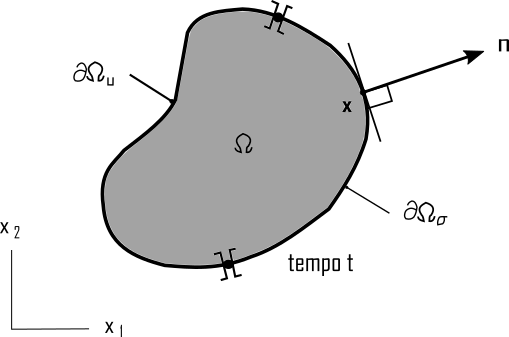
\includegraphics{images/CorpoCondCont.png}
	\label{fig:condcont}
	\fonte{O autor (2020)}
\end{figure}

As condições de contorno naturais ou condições de contorno de Von Neumann são identificadas fisicamente como trações de superfície. Elas são necessárias para a correta descrição do problema diferencial, sendo responsáveis pelas forças aplicadas ao corpo. Estas condições não atuam na variável primal. Elas atuam no campo de tensões, que é função do campo de deslocamentos através da relação ou modelo constitutivo usado. As condições de contorno naturais podem ser descritas da seguinte forma.

\begin{equation}
	\boldsymbol{t} = \boldsymbol{\sigma}\boldsymbol{n} = \boldsymbol{\overline{t}} \quad \forall \; \boldsymbol{x} \; \in \; \partial \Omega_{\sigma}
\end{equation}

Agora todas as expressões necessárias para uma definição bem posta de um problema diferencial estão disponíveis. De acordo com \cite{Paulo} neste estado o problema está na forma chamada forte, pois fornece a solução exata restringindo as possíveis soluções ao conjunto de funções $C1$. \footnote{Conjunto de funções onde, além de outras exigências, a primeira derivada deve ser contínua.} O problema a ser resolvido na forma forte é o seguinte:
\begin{align}
    \begin{cases}
	div\boldsymbol{\sigma(\boldsymbol{u})} + \boldsymbol{b} = \rho \ddot{\boldsymbol{u}}\\
	u = \overline{u} \quad \forall \; \boldsymbol{x} \; \in  \partial \Omega_u\\
	\boldsymbol{t} = \boldsymbol{\sigma}\boldsymbol{n} = \boldsymbol{\overline{t}} \quad \forall \; \boldsymbol{x} \; \in \; \partial \Omega_{\sigma} \\
	\boldsymbol{u}(\boldsymbol{x},t)|_{t=0} = \boldsymbol{u}_{0}(\boldsymbol{x}) \\
	\dot{\boldsymbol{u}}(\boldsymbol{x},t)|_{t=0} = \dot{\boldsymbol{u}_{0}}(\boldsymbol{x})
	\end{cases}
\end{align}

A solução de um problema na forma forte deve ser obtida através de procedimentos analíticos, já que este é contínuo. Por conta disto, a resolução deste problema em domínios arbitrários não é trivial. De acordo com \cite{Paulo} a forma forte deve ser transformada em uma forma chamada fraca, para então ser discretizada e resolvida numericamente.

\subsection{A forma fraca}
A construção da forma fraca será feita pelo principio dos trabalhos virtuais, conhecido como PTV. O primeiro passo para tal é multiplicar a equação por uma função vetorial arbitrária, que é representada por $ \boldsymbol{\hat{u}} = \boldsymbol{\hat{u}}(\boldsymbol{x})  $ e é chamada função teste ou de deslocamentos virtuais. Ao integrar, ao longo de todo o corpo, o resultado da operação anterior é obtida a equação \ref{eq:formafraca1}.
\begin{equation}
\int_{\Omega} div(\boldsymbol{\sigma}) \cdot \boldsymbol{\hat{u}} + \boldsymbol{b} \cdot \boldsymbol{\hat{u}} - \rho\ddot{\boldsymbol{u}} \cdot \boldsymbol{\hat{u}} \; dV = 0
\label{eq:formafraca1}
\end{equation}

De acordo com \cite{Holzapfel} o próximo passo é aplicar a regra do produto, usando a simetria do tensor de tensões de Cauchy. Com isso, é possível trabalhar o primeiro termo da integral em \ref{eq:formafraca1} da seguinte forma.\footnote{Esta passagem não é trivial, porém a expressão da regra do produto usada pode ser encontrada sem derivação em \cite{Holzapfel} equação 1.290}
\begin{equation}
	div \boldsymbol{\sigma} \cdot \boldsymbol{\hat{u}} = div(\boldsymbol{\sigma}\boldsymbol{\hat{u}}) - \boldsymbol{\sigma} : grad \boldsymbol{\hat{u}}
	\label{eq:formafraca2}
\end{equation}

Ao aplicar o teorema do divergente, a propriedade comutativa do produto interno e novamente a simetria do tensor de tensões de Cauchy no primeiro termo do braço direito da equação \ref{eq:formafraca2}. Obtêm-se a seguinte expressão.
\begin{equation} \label{eq:formafracatrans}
	\int_{\Omega} div(\boldsymbol{\sigma \hat{u}}) dV = \int_{\partial \Omega} \boldsymbol{\sigma \hat{u}} \cdot \boldsymbol{n} ds = \int_{\partial \Omega} \boldsymbol{\sigma n} \cdot \boldsymbol{\hat{u}} ds
\end{equation}

Ao substituir \ref{eq:formafracatrans} na equação \ref{eq:formafraca1}, é obtida a seguinte expressão.

\begin{equation}
\int_{\Omega} \boldsymbol{\sigma} : grad \boldsymbol{\hat{u}} -  \boldsymbol{b} \cdot \boldsymbol{\hat{u}} + \rho\ddot{\boldsymbol{u}} \cdot \boldsymbol{\hat{u}} dV - \int_{\partial \Omega} \boldsymbol{\sigma n} \cdot \boldsymbol{\hat{u}} ds = 0
\label{eq:formafraca3}
\end{equation}

Para continuar a derivação é necessária uma discussão sobre \gls{u} e \gls{uvir}.  Assim como aponta \cite{Paulo} o campo de deslocamentos pertence ao conjunto de funções cinematicamente admissíveis, definido por 
\begin{equation}
	Kin = \{ \boldsymbol{u}(\boldsymbol{x},t) \; é \; suficientemente \; regular \; tal \; que \; \boldsymbol{u}(\boldsymbol{x},t) = \boldsymbol{\overline{u}}  \quad \forall \boldsymbol{x} \in \partial \Omega_u \}
\end{equation}

Já os deslocamentos virtuais chamados anteriormente de arbitrários devem pertencer ao chamado espaço das variações.
\begin{equation}
	Var  = \{ \boldsymbol{\hat{u}}(\boldsymbol{x}) \; é \; suficientemente \; regular \; tal \; que \; \boldsymbol{\hat{u}}(\boldsymbol{x}) = 0  \quad \forall \boldsymbol{x} \in \partial \Omega_u \}
\end{equation}


De acordo com \cite{Paulo} agora ao destaca-se a segunda integral da equação \ref{eq:formafraca3}, considerando que $ \boldsymbol{\overline{u}} = 0 \quad \forall \boldsymbol{x} \in \partial \Omega_u $ e sabendo que $ \boldsymbol{\sigma n} = \boldsymbol{\overline{t}} \quad \forall \in \partial \Omega_{\sigma} $.

\begin{equation} \label{eq:formafracatrans}
	\int_{\partial \Omega} \boldsymbol{\sigma n} \cdot \boldsymbol{\hat{u}} ds = \int_{\partial \Omega_u} \boldsymbol{\sigma n} \cdot \boldsymbol{0} ds + \int_{\partial \Omega_{\sigma}} \boldsymbol{\overline{t}} \cdot \boldsymbol{\hat{u}} ds = \int_{\partial \Omega_{\sigma}} \boldsymbol{\overline{t}} \cdot \boldsymbol{\hat{u}} ds 
\end{equation}

A forma fraca do problema é finalmente caracterizada pela seguinte expressão, onde \ref{eq:formafracatrans} foi inserido em \ref{eq:formafraca3}.

\begin{equation} \label{eq:formafracafinal}
	\int_{\Omega} \boldsymbol{\sigma} : grad \boldsymbol{\hat{u}} -  \boldsymbol{b} \cdot \boldsymbol{\hat{u}} +  \rho\ddot{\boldsymbol{u}} \cdot \boldsymbol{\hat{u}}  dV - \int_{\partial \Omega_{\sigma}} \boldsymbol{\overline{t}} \cdot \boldsymbol{\hat{u}} ds = 0 
\end{equation}

De acordo com \cite{Paulo} a função de teste $ \hat{u} $ tem um significado especial no principio dos trabalhos virtuais. Ela é chamada de deslocamentos virtuais e forma trabalhos virtuais quando associada às forças internas e externas. A identificação dos termos da forma fraca, de acordo com o princípio dos trabalhos virtuais, é feita a seguir.
\begin{itemize}
	\item Trabalho virtual interno
	\begin{equation}
		\int_{\Omega} \boldsymbol{\sigma} : grad\boldsymbol{\hat{u}} dV
	\end{equation}
	\item Trabalho virtual externo
	\begin{equation}
		\int_{\Omega} \boldsymbol{b} \cdot \boldsymbol{\hat{u}} dV + \int_{\partial \Omega_{\sigma}} \boldsymbol{\overline{t}} \cdot \boldsymbol{\hat{u}} d\partial \Omega_{\sigma}
	\end{equation}
	\item Termo relacionado à inercia
	\begin{equation}
		\int_{\Omega} \rho \ddot{\boldsymbol{u}} \cdot \boldsymbol{\hat{u}}  dV
	\end{equation}
\end{itemize}

Antes de partir para a solução da forma fraca, é preciso esclarecer se ela é válida para resolver a forma forte. Pelo lema fundamental do cálculo variacional:\\
Dada uma função $ f(x) $ contínua, se
\begin{equation}
\int_{a}^{b} f(x) h(x) dx = 0
\end{equation}
para toda e qualquer função arbitrária $ h(x) $,
então $ f(x) = 0 $ no intervalo (a,b). \\

A partir de \ref{eq:formafraca1}, reduzindo a equação para a forma unidimensional, é evidenciado que o lema fundamental apresentado acima evidencia que a forma forte é resolvida pela forma fraca.
\begin{align}
	\int_{\Omega} \frac{\partial \sigma_x}{\partial x} \hat{u} + b_x \hat{u} - \rho\ddot{u} \hat{u} \; dx = 0 \\
	\int_{\Omega} (\frac{\partial \sigma_x}{\partial x}  + b_x - \rho\ddot{u} )\hat{u} \; dx = 0
\end{align}

\subsection{A Discretização no espaço}

Para resolver a forma fraca é necessário discretizar o domínio no espaço. A descrição em uma dimensão será usada, todavia os conceitos apresentados são iguais independente de quantas dimensões são empregadas. O domínio representado pelo conjunto (a,b) é contínuo, portanto de acordo com \cite{Paulo} tem dimensão infinita. Este deve ser dividido em regiões menores, de forma que.
\begin{equation} \label{eq:malha1d}
	x_1 = a \quad x_i<x_{i+1} \quad e \; x_N = b
\end{equation}

Em uma dimensão cada intervalo de $ x_i $  a $ x_{i+1} $ define um elemento do domínio. A soma de todos os elementos, em conjunto com o contorno, compõe o domínio do problema que agora é finito. Os pontos $ x_i $ são chamados de nós, e a união entre elementos e nós forma uma malha. \\

A aproximação das funções $ u(x,t) \; e \; \hat{u}(x,t) $ é feita da seguinte maneira.
\begin{align} 
	u(x,t) \approx u_h(x,t) = \sum_{n=1}^{N} \phi_n (x) u_n(t) \\
	\hat{u}(x,t) \approx \hat{u}_h(x) = \sum_{m=1}^{N} \phi_m (x) \hat{u}_m  
\end{align}

Onde $ u_n $ e $ \hat{u}_m $ são valores nodais dos respectivos campos.
De acordo com \cite{zienkiewicz2013} considerando a malha expressa por \ref{eq:malha1d}, é possível definir o conjunto de funções polinomiais de aproximação a seguir.

\begin{equation} \label{eq:funcform}
    \phi_i =  \left \{ \begin{array}{rcl}
         0, & \text{se} & x < x_{i-1} \\
        \ddfrac{x - x_{i-1}}{x_i - x_{i-1}}, &  \text{se} & x_{i-1} < x < x_{i} \\
        \ddfrac{x_{i+1} - x}{x_{i+1} - x_{i}}, &  \text{se} & x_i < x < x_{i+1} \\
         0, & \text{se} & x > x_{i+1}
    \end{array} \right.
\end{equation}

\begin{figure}[h] % TODO: Inserir fonte \cite{zienc}
    \centering
    \caption{ a: Funções de aproximação descritas em \ref{eq:funcform}. b: Derivadas das mesmas funções }
    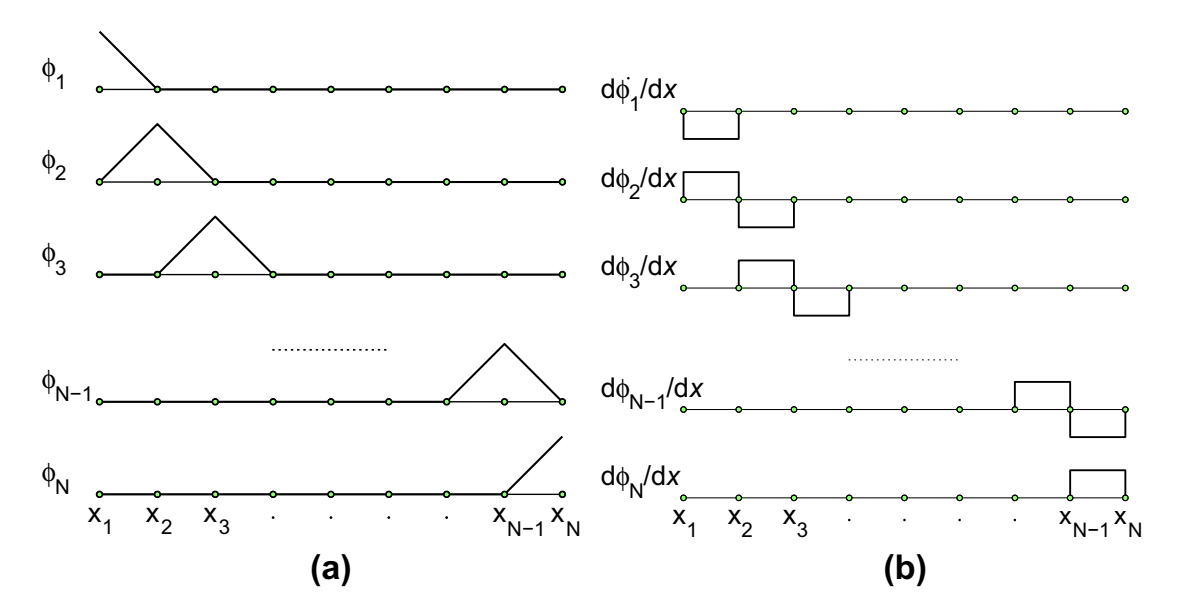
\includegraphics[width=0.8\linewidth]{images/funcform.png}
    \label{fig:funcform}
    \fonte{\cite{zienkiewicz2013}}
\end{figure}

A figura \ref{fig:funcform} mostra as funções definidas em \ref{eq:funcform}. De acordo com \cite{zienkiewicz2013} estas funções são pertencentes ao conjunto $C0$, portanto são simplesmente contínuas. Sendo assim, suas derivadas são apenas contínuas por partes.

De acordo com \cite{zienkiewicz2013}. ao considerar que o modelo constitutivo é a lei de Hooke, que o corpo tem coeficiente de Poisson nulo e que cargas superficiais não estão presentes. A forma fraca unidimensional é descrita da seguinte forma.\footnote{Considerar Poisson nulo, neste caso, permite que exista apenas a componente $ \sigma_x $} \footnote{De acordo com a lei de Hooke $ \sigma_x = E \varepsilon_x = E \frac{\partial u}{ \partial x} $}
\begin{equation} \label{eq:formafracalin}
    \int_{\Omega} \hat{u} (\rho \ddfrac{\partial^2 u}{\partial t^2} - b_x) \, dx + \int_{\Omega} \ddfrac{\partial \hat{u}}{\partial x} E \ddfrac{\partial u}{ \partial x} \,  dx
\end{equation}

De acordo com \cite{zienkiewicz2013}  as integrais no domínio do corpo podem ser computadas da seguinte forma

\begin{equation} \label{eq:integraisdif}
    \int_{\Omega} (\cdot) \, dx = \sum_{i = 1}^{N_{el}} \int_{x_i}^{x_{i+1}} (\cdot) \, dx \equiv \sum_{e} \int_{\Omega_e} (\cdot) dx
\end{equation}

Onde $ N_{el} $ é o número de elementos, e $\sum_e$ é um somatório que compreende todos os elementos. A última integral em \ref{eq:integraisdif} mostra que é possível calcular a participação de cada elemento, desta forma a integral no domínio é a soma das participações dos elementos. O criador de um dos maiores softwares de código aberto em elementos finitos, autor de  \cite{BangerthHartmannKanschat2007}, afirma em uma de suas videoaulas que a capacidade de tratar de forma igualitária cada elemento é uma das maiores vantagens computacionais do método dos elementos finitos.\footnote{O sitio para acesso das videoaulas é \url{https://www.math.colostate.edu/~bangerth/videos.html}} \\

\begin{figure}
    \centering
    \caption{a: Funções de forma para um certo elemento. b: Derivadas das mesmas funções}
    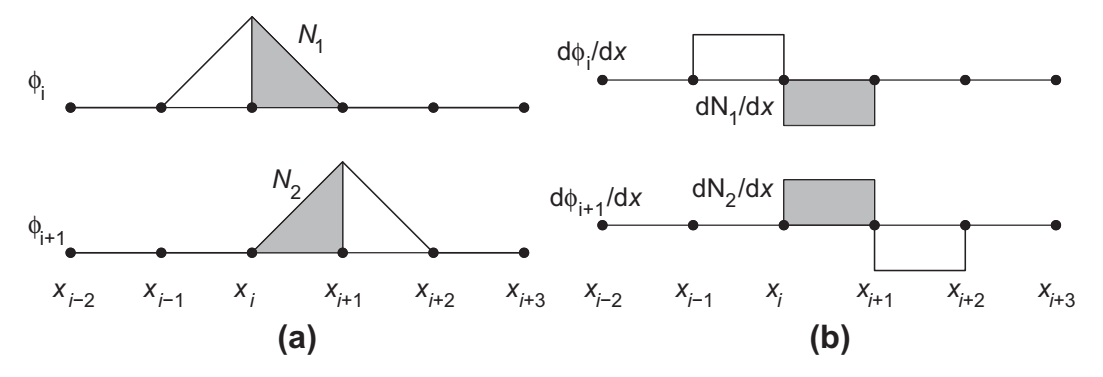
\includegraphics[width=0.8\linewidth]{images/funcformaverdade.png}
    \label{fig:funcformverd}
    \fonte{\cite{zienkiewicz2013}}
\end{figure}

De acordo com \cite{zienkiewicz2013} todos os elementos ou intervalos $ [x_i, x_{i+1}] $ presentes na figura \ref{fig:funcformverd} usam as mesmas funções $ N_1 $  e $ N_2 $ para sua definição, portanto estas são chamadas funções de forma para o elemento. Um elemento é chamado de linear ou quadrático quando suas funções de forma são lineares ou quadráticas e assim por diante. As seguintes propriedades são válidas e necessárias para as funções de aproximação, que dentro de um elemento são chamadas de função de forma, de acordo com \cite{Paulo}.

\begin{itemize}
    \item Uma função associada a um certo nó $ i $ é nula em todos os outros nós da malha.
    \item Cada função $ \phi_i $ é nula em todos os elementos que não contém o nó $i$.
    \item A soma de todas as funções de aproximação em um ponto qualquer é \begin{equation}
        \sum^N_{n=i} \phi_n (x) = 1
    \end{equation} um conjunto de funções que satisfazem essa propriedade são ditas partição da unidade. 
\end{itemize}

Dado que a integral é feita em cada elemento  um sistema de coordenadas locais é inserido, nele
\begin{equation}
    x' =  x - x^e_1 
\end{equation}

na qual $ x^e_1 $ é a coordenada do primeiro nó de um elemento $e $, $x$ é a coordenada global e $x'$ a coordenada local. De acordo com \cite{zienkiewicz2013}, ao aplicar o sistema de coordenadas local nas funções de forma. As aproximações dos campos de deslocamento e de deslocamento virtual são escritas da seguinte maneira

\begin{align}
    u_h^e = N_1(x')u_1^e + N_2(x')u_2^e \\
    \hat{u}_h^e = N_1(x')\hat{u}_1^e + N_2(x')\hat{u}_2^e
\end{align}

Onde $ u^e_i $ e $ \hat{u}^e_i $ é a aproximação do respectivo campo $ u $ ou $ \hat{u} $ no nó $ i $ do elemento $ e $. Ao aplicar estas aproximações na forma fraca apresentada em \ref{eq:formafracalin}, seguida da separação dos termos de acordo com sua contribuição energética. De acordo com \cite{zienkiewicz2013}, são formadas as seguintes expressões

\begin{itemize}
    \item Termo relacionado à inercia: \begin{equation}
        \sum_{e=1}^M [\hat{u}^e_1 \, \hat{u}^e_2 ] \int_{\Omega_e} \begin{Bmatrix} N_1 \\ N_2 \end{Bmatrix} \rho \begin{Bmatrix} N_1 & N_2 \end{Bmatrix} \; dx' \begin{Bmatrix} \ddot{u}^e_1 \\ \ddot{u}^e_2 \end{Bmatrix}
    \end{equation}
    
    \item Termo relacionado à tensão interna \begin{equation}
        \sum_{e=1}^M [\hat{u}^e_1 \, \hat{u}^e_2 ] \int_{\Omega_e} \begin{Bmatrix} \ddfrac{dN_1}{dx'} \\ \ddfrac{dN_2}{dx'}  \end{Bmatrix} E \begin{Bmatrix} \ddfrac{dN_1}{dx'}  & \ddfrac{dN_2}{dx'}  \end{Bmatrix} \; dx' \begin{Bmatrix} u^e_1 \\ u^e_2 \end{Bmatrix}
    \end{equation}
    
    \item Termo relacionado às forças de corpo: 
    \begin{equation}
        \sum_{e=1}^M [\hat{u}^e_1 \, \hat{u}^e_2 ] \int_{\Omega_e} \begin{Bmatrix} N_1 \\ N_2  \end{Bmatrix} b_x \; dx'
    \end{equation}
\end{itemize}

Avaliando as integrais dos termos acima são obtidas matrizes e vetores pertencentes ao elemento $e$. Computar as integrais apresentadas aqui é trivial, já que as expressões foram extremamente simplificadas. Em um problema com duas ou três dimensões calcular analiticamente as integrais formadas não é factível. De acordo com \cite{zienkiewicz2013} o cálculo das integrais frmadas é feito usando integrações numéricas chamadas de quadraturas.\footnote{A quadratura mais usada é a de Gauss-Legendre, explicações sobre as quadraturas e suas peculiaridades são encontradas em \cite{Paulo} e \cite{zienkiewicz2013}} As matrizes de massa e rigidez, assim como o vetor de forças de corpo são resultados do cálculo das integrais previamente citadas. 

\begin{itemize}
    \item Matriz de massa do elemento : \begin{equation} \boldsymbol{M}^e = \int_{\Omega_e} \begin{Bmatrix} N_1 \\ N_2 \end{Bmatrix} \rho \begin{Bmatrix} N_1 & N_2 \end{Bmatrix} \; dx' = \begin{bmatrix} M^e_{11} & M^e_{12} \\ M^e_{21} & M^e_{22} \end{bmatrix} \end{equation} 
    \item Matriz de rigidez do elemento: \begin{equation}
        \boldsymbol{K}^e = \int_{\Omega_e} \begin{Bmatrix} \ddfrac{dN_1}{dx'} \\ \ddfrac{dN_2}{dx'}  \end{Bmatrix} E \begin{Bmatrix} \ddfrac{dN_1}{dx'}  & \ddfrac{dN_2}{dx'}  \end{Bmatrix} \; dx' = \begin{bmatrix} K^e_{11} & K^e_{12} \\ K^e_{21} & K^e_{22} \end{bmatrix}
    \end{equation}
    
    \item Vetor de forças de corpo do elemento: 
    \begin{equation}
        \boldsymbol{F}^e = \int_{\Omega_e} \begin{Bmatrix} N_1 \\ N_2  \end{Bmatrix} b_x \; dx' = \begin{bmatrix} F^e_1 \\ F^e_2 \end{bmatrix}
    \end{equation}
\end{itemize}

 De acordo com \cite{Paulo} ao considerar que  $ \hat{u} \neq 0 $, além disso somando todas as participações dos elementos. O sistema torna-se uma equação algébrica, vide equação \ref{eq:formafindiscesp}.

\begin{equation} \label{eq:formafindiscesp}
    \boldsymbol{M \ddot{u} } + \boldsymbol{Ku} = \boldsymbol{F}
\end{equation}

Sendo $ \boldsymbol{M} $ e $ \boldsymbol{K} $ as matrizes de massa e rigidez, $\boldsymbol{F}$ o vetor de forças de corpo, $ \boldsymbol{\ddot{u}} $ o vetor das acelerações nodais e $\boldsymbol{u}$ o vetor de deslocamentos nodais.\\

A equação algébrica \ref{eq:formafindiscesp} é a forma final da discretização espacial de um sistema linear.

\subsubsection{A discretização de um problema dinâmico}

A discretização de um problema dinâmico tem algumas particularidades a serem consideradas. Uma delas é chamada de trancamento ou em inglês "Locking". De acordo com \cite{Paulo} o trancamento é observado em elementos lineares contendo todos os pontos de integração, estes pontos são oriundos da integração numérica usada na solução. O trancamento se manifesta através de um excesso de rigidez na malha, por conseguinte os deslocamentos são subestimados e o resultado é fisicamente inválido. \\

A técnica de integração numérica mais usada é a quadratura de Gauss-Legendre. Um polinômio de grau $p$ necessita de $np$ pontos em sua integração para ser integrado de forma exata, de acordo com a equação \ref{eq:quadratu}. 
\begin{equation} \label{eq:quadratu}
    P=2np-3
\end{equation}

De acordo com \cite{Paulo} são necessários oito pontos para integrar exatamente um elemento hexaédrico de oito nós, representado na figura \ref{fig:hexaoito}. Este elemento usa funções lineares semelhantes às funções apresentadas no exemplo unidimensional, porém sua dimensão faz com que estejam presentes funções de grau 2 na integral do elemento. Os pontos de integração estão representados na figura  \ref{fig:hexapontos}. \\
\begin{figure}
\caption{Elemento hexaédrico de oito nós e seus pontos de integração.}

\begin{subfigure}{0.5\textwidth}
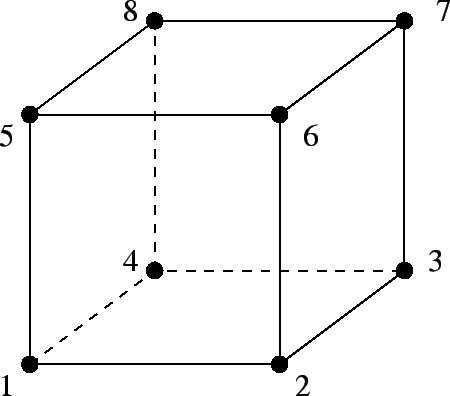
\includegraphics[width=0.9\linewidth, height=5cm]{images/hexapointsofint.png}
    \caption{Elemento hexaédrico de oito nós}
    \label{fig:hexaoito}
\end{subfigure}
\begin{subfigure}{0.5\textwidth}
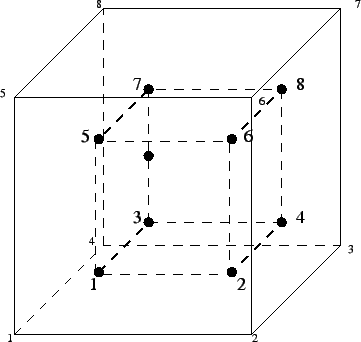
\includegraphics[width=0.9\linewidth, height=5cm]{images/hexaelement.png}
\caption{Pontos de integração do elemento}
\label{fig:hexapontos}
\end{subfigure}
\label{fig:hexaele}

\fonte{ \url{http://web.mit.edu/calculix_v2.7/CalculiX/ccx_2.7/doc/ccx/node26.html}}
\end{figure}
%CONTINUAR REVISAO%

A integração completa, ou seja integrar usando todos os pontos provenientes da quadratura, de elementos lineares pode gerar trancamento. Além disso, o custo computacional deste tipo de integração é extremamente alto, dado que malhas com elementos muito pequenos são necessárias para a correta solução de um problema de impacto balístico. A solução encontrada é uma técnica chamada subintegração. Ela consiste em usar menos pontos de integração do que seriam necessários para o elemento. No caso dinâmico é costumeiro usar apenas um ponto e este é localizado no centro do elemento. De acordo com \cite{theorymanls} os elementos com um ponto de integração são 25 vezes menos custosos em termos computacionais, em relação aos totalmente integrados. Embora a subintegração diminua o custo computacional e resolva o trancamento ela não é a solução perfeita, já que este tipo de técnica tem problemas colaterais associados a seu uso. \par

Os problemas gerados pela subintegação são a representação da tensão como um tensor constante no elemento e o surgimento de modos espúrios de deformação. A representação da tensão como constante não é um grande problema, já que um refino de malha é suficiente para sua solução. Os modos espúrios de deformação causam muito mais dor de cabeça ao analista. O que acontece é que os elementos se deformam sem gastar energia e com isso geram ruídos na energia total do sistema, portanto é necessário controla-los. Estes modos espúrios de deformação são chamados de ampulheta ou "Hourglass". O nome ampulheta se dá por conta do formato assumido pelo conjunto de dois elementos quando estão se deformando em modo espúrio, vide figura \ref{fig:hourglass}. 

\begin{figure}
    \centering
    \caption{Deformação espúria formando uma ampulheta entre os elementos.}
    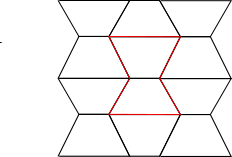
\includegraphics[width=0.5\linewidth]{images/hourglass.png}
    \label{fig:hourglass}
    \fonte{O autor (2020)}
\end{figure}

\subsection{A discretização no tempo}

A equação algébrica \ref{eq:formafindiscesp} está discretizada no espaço, porém note que não foi feita qualquer consideração quanto ao tempo. É necessário discretizar esta equação no tempo e isso é feito usando um método de marcha. De acordo com \cite{Paulo} este nome vem do fato de que o tempo é subdividido em intervalos e um algoritmo passa por cada um deles de forma sequencial. O intervalo de tempo considerado é $[t_0,t_f] $ . A marcha ocorrerá de forma a passar por um intervalo $ \Delta t $ a cada iteração, sendo $ t_1 = t_0 + \Delta t $, $ t_2 = t_0 + 2 \Delta t = t_1 + \Delta t $ e assim por conseguinte. Existem dois grupos de métodos usados para realizar esta marcha no tempo, são eles implícitos e explícitos. \\

A escolha entre os métodos leva em consideração o comportamento esperado da solução, que pode ser classificado de acordo com o formato da equação diferencial resolvida. De acordo com \cite{BangerthHartmannKanschat2007} a equação de onda é classificada como hiperbólica, logo não é esperada a atenuação da curva descrita pela variável essencial. Um impacto em alta velocidade excita frequências altas dos corpos envolvidos, assim é necessário que o passo de tempo seja pequeno para que as influências destas faixas de frequência sejam corretamente computadas. O custo computacional de cada $\Delta t$ em um método implícito é muito mais alto do que em um método explícito, no entanto estes métodos são incondicionalmente estáveis. Dizer que o método é incondicionalmente estável significa que é possível usar passos de tempo tão grandes quanto desejado. Em um método condicionalmente estável há uma limitação quanto ao passo usado, nestes é preciso reduzir o $ \Delta t $ de acordo com a equação \ref{eq:defdeltat}. Onde $l$ é a menor dimensão de um elemento da malha, $c$ é a velocidade do som no material e $k$ é um fator de estabilidade que normalmente varia entre 0.6 e 0.9. \\


Para o caso de impactos balísticos, que envolvem velocidades relativamente altas, os métodos explícitos são mais interessantes. Conforme \cite{Zukas} o uso de grandes passos de tempo faz com que detalhes da solução sejam perdidos, logo não seria possível extrair benefício da estabilidade incondicional dos métodos implícitos e métodos explícitos são preferidos por seu custo inferior. \\

\begin{equation}
\Delta t = \frac{k l }{c}
\label{eq:defdeltat}
\end{equation}

A equação \ref{eq:formafindiscesp} é escrita da seguinte forma
    \begin{equation} \label{eq:formainicialdisctempo}
    \boldsymbol{M \ddot{u}_n } + \boldsymbol{K}\boldsymbol{u}_n = \boldsymbol{F}_n
\end{equation}
Onde $ u_n $ é o deslocamento em $t=n$, portanto a equação \ref{eq:formainicialdisctempo} descreve o sistema em um determinado tempo $t_n $. È necessário que todos os valores sejam conhecidos em e até $ t_n $. As condições iniciais são usadas para caracterizar o sistema em $ t_0 $. Para avançar no tempo o método das diferenças centrais toma a velocidade média em cada intervalo da seguinte forma

\begin{align} \label{eq:vels}
    \dot{u}_{n-\frac{1}{2}} \approx \ddfrac{u_n - u_{n-1}}{\Delta t} & \hspace{25mm} \text{e} & \dot{u}_{n+\frac{1}{2}} \approx \ddfrac{ u_{n+1} + u_n}{\Delta t} 
\end{align} 

Usando as velocidades definidas em \ref{eq:vels} é possível escrever a aceleração $ \ddot{u}_n $ 

\begin{equation} \label{eq:acels}
    \ddot{u} = \ddfrac{u_{n+1} - 2u_n + u_{n-1}}{\Delta t^2}
\end{equation}

Agora substituindo \ref{eq:acels} em \ref{eq:formainicialdisctempo} a seguinte expressão é alcançada.

\begin{equation} \label{eq:formaquasefimdisctempo}
    \ddfrac{1}{\Delta t^2}\boldsymbol{M} \boldsymbol{u_{n+1}} = [\boldsymbol{F}_n - \boldsymbol{Ku}_n + \ddfrac{1}{\Delta t^2}\boldsymbol{M}(2\boldsymbol{u}_n - \boldsymbol{u}_{n-1}) ]
\end{equation}

Para transformar \ref{eq:formaquasefimdisctempo} em sua forma explícita é necessário realizar o procedimento de diagonalização da matriz de massa, que faz com que todos os termos sejam transferidos para a diagonal principal. De acordo com \cite{Paulo} este procedimento implica perda de informação, o que gera erros adicionais de aproximação. Porém para que o procedimento de diagonalização seja válido se faz necessário que a massa de cada elemento seja conservada. Depois da diagonalização a equação \ref{eq:formaquasefimdisctempo} assume sua forma final e por sua vez explícita, já que de acordo com \cite{Paulo} não há necessidade de se resolver um sistema algébrico.

\begin{equation}
    u^j_{n+1} = (\ddfrac{M_{jj}}{\Delta t^2} )^-1 [F_n^j - (Ku_n)^j + \ddfrac{1}{\Delta t^2}M_{jj}(2u_n^j - u_{n-1}^j) + \ddfrac{1}{2 \Delta t}C u_{n-1}]
\end{equation}


\chapter{Os modelos constitutivos} \label{Cap: ModConst}

Em eventos onde deformações inelásticas estão presentes as tensões são modeladas de forma decomposta. De acordo com \cite{Holzapfel} todo tensor pode ser decomposto de forma aditiva em uma parcela esférica e uma desviadora. No caso dos tensores de tensão, a parcela esférica é oriunda de deformações que alteram o volume e a desviadora advém de deformações isocóricas. A decomposição aditiva do tensor de tensões de Cauchy é apresentada a seguir

\begin{equation} 
    \boldsymbol{\sigma} = \boldsymbol{s} - p\boldsymbol{I}
\end{equation}

Nela $ \gls{I} $ é o tensor identidade, $\boldsymbol{s}d$ é a parcela desviadora das tensões e $p$ é a pressão. Em eventos onde há presença de ondas de choque, a parte isocórica do tensor de tensões é modelada por uma equação constitutiva e a parte esférica por uma equação de estado. Antes de apresentar os modelos constitutivos mais usados é importante visitar alguns pontos da teoria da plasticidade, já que ela terá grande importância na definição do comportamento dos materiais quando submetidos à cargas elevadas. \\

De acordo com \cite{hiermaier_2008} a deformação irreversível de materiais é resultado de alterações na sua microestrutura. Destacam-se o movimento de discordâncias, o crescimento e o coalescimento de micro vazios como mecanismos citados por \cite{hiermaier_2008}. Estas alterações microestruturais são causadas por solicitações que elevam o material a tensões superiores à de resistência ao escoamento. De acordo com \cite{tadmor_miller_elliott_2012} a mecânica do contínuo não toma conhecimento da estrutura do material para descrever seu comportamento. Tal consideração faz com que fenômenos de ordem microestrutural não sejam levados em consideração direta, no entanto eles são considerados de forma indireta por meio de variáveis de estado internas, usadas nos modelos constitutivos. \\

De acordo com \cite{Holzapfel} as variáveis internas não podem ser mensuradas em um ensaio, porém são usadas para descrever o estado do material. O comportamento mecânico do material é associado ao seu estado, por exemplo: A tensão é calculada em função das variáveis de estado, por meio da relação constitutiva. Um exemplo de variável interna, que pode ser usada para descrever o estado e por conseguinte o comportamento do material, é o dano. Ele é calculado por vários modelos e em alguns deles é usado para definir a resistência do material, porém não há como medi-lo diretamente em um laboratório. \\

 A avaliação do comportamento esperado para o material deve considerar os pormenores de seu estado para saber se as alterações no ambiente ou no tipo de solicitação fazem com que haja mudança nas propriedades previamente observadas. De acordo com \cite{Zukas} dados obtidos em condições de baixa pressão e em situações quasi-estáticas dificilmente serão uteis para a simulação de um evento em alta velocidade. \par

As propriedades dos materiais podem apresentar grandes diferenças quando diferentes taxas de deformação são aplicadas. No extremo inferior da taxa de deformação a fadiga pode estar presente caso as condições de temperatura e carga sejam propicias. No extremo superior, a solicitação de materiais devido à explosões faz com que a resistência do material possa ser completamente ignorada, quando estes eventos são simulados. Este trabalho busca apresentar os modelos constitutivos inseridos no contexto de impactos de media velocidade. Por média velocidade entende-se que os impactos não levam o material ao estado de choque. De acordo com \cite{Zukas} este tipo de impacto são são aqueles onde a velocidade do projetil não supera os $2000 m/s$. De acordo com \cite{Hazell} a velocidade limítrofe para o inicio da observação de ondas de choque depende do material impactado, elas surgem quando a velocidade de penetração supera a velocidade do som no meio. \par


Quando não há presença de ondas de choque, o material pode ser modelado apenas por uma relação constitutiva ou por uma relação constitutiva e uma equação de estado, além disso equações de estado muito mais simples podem ser usadas neste tipo de situação. De acordo com \cite{hiermaier_2008} a plasticidade computacional oferece base teórica para os modelos constitutivos usados na balística. \\

\section{Plasticidade perfeita, isotrópica e cinemática.}

De acordo com \cite{neto_peric_owens_2008} quando um corpo se deforma plasticamente ele pode apresentar, um ou uma mistura destes três tipos de plasticidade. 
\begin{itemize}
    \item Plasticidade perfeita.
    \item Plasticidade Isotrópica
    \item Plasticidade cinemática.
\end{itemize}
\par

A plasticidade perfeita é caracterizada pela estabilidade da tensão de escoamento. Nela o material escoa sem aumentar a resistência a futuras deformações plásticas. Uma curva de carga e descarga que apresenta plasticidade perfeita pode ser vista na figura \ref{fig:plastperf}. Não há alteração da tensão de escoamento, tal comportamento independe da quantidade de deformação que o material sofre. \\ 
\begin{figure}[H]
    \centering
    \caption{Curva de tensão deformação apresentando plasticidade perfeita. }
    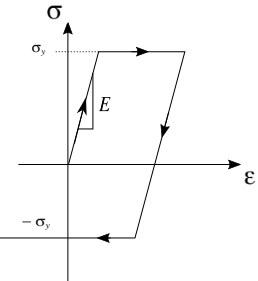
\includegraphics[width=0.5\linewidth]{images/plasticidade_perfeita.png}
    \label{fig:plastperf}
    \fonte{O autor (2020)}
\end{figure}

O segundo comportamento típico é a plasticidade isotrópica. Nela a tensão limite de escoamento é alterada por conta de deformações plásticas. Portanto, caso uma tensão trativa gerar deformação plástica em um ponto, um subsequente ciclo de carregamento necessitará de maior tensão trativa para gerar deformação plástica neste mesmo ponto. O característico da plasticidade isotrópica é que o aumento do limite de escoamento em tração significa também um aumento do limite de escoamento em compressão.
Portanto, como mostra a figura \ref{fig:plastiso}, um ciclo de carregamento em tração gera deformação plástica, aumentando o limite de escoamento tanto em tração quanto em compressão. Um ciclo subsequente em compressão precisará atingir a tensão de escoamento inicial $\sigma_y$ somada a um delta de tensão $d\sigma$ para provocar deformação plástica. 

\begin{figure}[H]
    \centering
    \caption{Curva de tensão deformação apresentando plasticidade isotrópica. }
    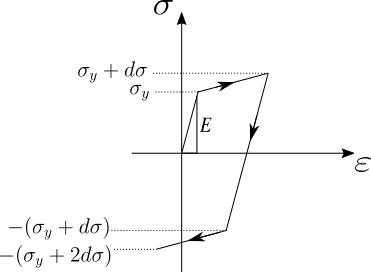
\includegraphics[width=0.5\linewidth]{images/plasticidade_iso.png}
    \label{fig:plastiso}
    \fonte{O autor (2020)}
\end{figure}

O último modo de plasticidade é a cinemática, nela a tensão limite de escoamento também é alterada de acordo com o nível de deformação plástica do material. Entretanto, a distância entre a tensão limite de escoamento em tração e em compressão se mantém igual ao longo do tempo. Portanto, um acréscimo na resistência à tensão trativa significa um decréscimo correspondente na resistência à tensão compressiva, vide figura \ref{fig:plastcin}.  \par

\begin{figure}[H]
    \centering
    \caption{Curva de tensão deformação apresentando plasticidade cinemática. }
    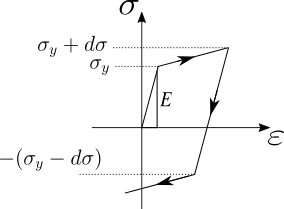
\includegraphics[width=0.5\linewidth]{images/plasticidade_cinem.png}
    \label{fig:plastcin}
    \fonte{O autor (2020)}
\end{figure}

Nos casos onde há alteração da tensão de escoamento, por conta da deformação plástica, é possível o endurecimento ou encruamento ocorra de forma linear ou não linear. A figura \ref{fig:plastlinvsnlin} exemplifica a diferença entre a plasticidade isotrópica linear e não linear. \par

\begin{figure}[H]
    \centering
    \caption{Comparação de encruamento linear versus não linear. } 
    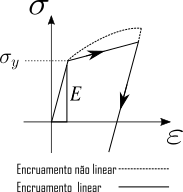
\includegraphics[width=0.8\linewidth]{images/plasticidade_linnlin.png}
    \label{fig:plastlinvsnlin}
    \fonte{O autor (2020)}
\end{figure}

Nada impede que estes comportamentos ocorram ao mesmo tempo. Portanto, um material pode, por exemplo, se comportar de forma isotrópica cinemática não linear. \\

\section{A superfície de escoamento e o espaço das tensões principais}

Até agora a tensão foi tratada como sendo escalar, portanto tratava-se da tensão observada em um estado uniaxial de tensão. \footnote{Aqui existe a repetição da palavra tensão pois o estado uniaxial de deformação existe e é importante no campo da balística.} O campo de tensões reais é descrito por um tensor, $ \gls{Cauchy} $, que contém nove componentes, sendo seis delas independentes entre si. O limite de escoamento, outrora escalar, agora é uma hiper superfície em seis dimensões. A descrição de um espaço hexa dimensional não é trivial, por conta disso, de acordo com \cite{hiermaier_2008},  foi criada uma descrição que usa a decomposição espectral do tensor de tensões.\footnote{O teorema responsável por tal decomposição é o teorema 
espectral e pode ser encontrado em \cite{gurtin_fried_anand_2013} pg. 28. } \\

O espaço característico do tensor de tensões é composto por seus auto vetores e auto valores. O teorema espectral torna possível escrever o tensor usando três componentes, que são posicionados na diagonal da matriz que representa o tensor. 
No contexto do tensor de tensões de Cauchy decomposto de forma espectral. Os auto valores são chamados de tensões principais e são os valores das componentes. Os auto vetores são representados pela linha da na matriz e são chamados de direções principais. Em forma matricial o tensor de tensões de Cauchy, descrito de forma espectral, é apresentado a seguir.

\begin{equation}
\gls{Cauchy} = 
    \begin{bmatrix}
    \sigma_1 & 0 & 0 \\
    0 & \sigma_2 & 0 \\
    0 & 0 & \sigma_3
    \end{bmatrix}
\end{equation}

Como dito anteriormente, é costumeiro decompor de forma aditiva o tensor de tensões. Esta decomposição é feita em duas parcelas, uma desviadora e a outra volumétrica. Portanto, apresenta-se a parcela desviadora do tensor de tensões quando decomposto de forma espectral.

\begin{equation}
\boldsymbol{S} = 
    \begin{bmatrix}
    S_1 & 0 & 0 \\
    0 & S_2 & 0 \\
    0 & 0 & S_3
    \end{bmatrix} = \begin{bmatrix}
    \sigma_1 - \sigma_m & 0 & 0 \\
    0 & \sigma_2 - \sigma_m & 0 \\
    0 & 0 & \sigma_3 - \sigma_m
    \end{bmatrix}
\end{equation}

Onde 
\begin{equation}
     \sigma_m = \frac{\sigma_1 + \sigma_2 + \sigma_3}{3}
\end{equation}

No espaço característico do tensor de Cauchy, a superfície de escoamento anteriormente em seis dimensões torna-se uma superfície em três dimensões, que pode ser descrita e entendida de forma mais simples. De acordo com \cite{hiermaier_2008} o espaço das tensões principais chama-se Espaço de Haigh-Westergaard, em referência aos pesquisadores que sugeriram tal descrição. Neste espaço o estado de tensões hidrostáticas é representado pela eq. \ref{eq:hydrostress}, onde $ J_1 $ é o primeiro invariante do tensor de tensões desviadoras. Neste estado as tensões desviadores $S_i$ são nulas, portanto a diagonal formada pela eq. \ref{eq:hydrostress} é chamada de eixo hidrostático.  

\begin{equation} \label{eq:hydrostress}
    \sigma_1 = \sigma_2 = \sigma_3 = \frac{1}{3} J_1
\end{equation}

Os invariantes $\gls{prinvadesv}$ das tensões desviadoras são usados para definir critérios de escoamento. Eles são aplicados nas funções que descrevem a superfície de escoamento. Existem algumas coordenadas que possuem leitura mais clara no espaço de haigh-Westergaard, que por sua vez são chamadas de coordenadas de Haigh-Westergaard. A descrição gráfica destas coordenadas é mostrada na figura \ref{fig:coordhaigh}. Uma explicação das coordenadas será dada a seguir, porém para tal é necessário definir o que são planos desviadores e meridianos. Planos desviadores são aqueles cuja normal é o eixo hidrostático, mover-se por um plano desviador significa alterar o estado de tensões desviadoras. Meridianos são perpendiculares aos planos desviadores e contém o eixo hidrostático, mover-se ao longo de um meridiano significa mudar o estado de tensão hidrostática mantendo constante a coordenada $\theta$. A figura \ref{fig:coordhaigh} apresenta tanto um plano desviador quanto um meridiano. \\

\begin{itemize}
    \item $ \xi $: Tem relação direta com o estado de pressão do material, portanto acompanha o eixo hidrostático.
    \item $ \rho $: Medida da distância do eixo hidrostático até a superfície de escoamento em um plano desviador.
    \item $ \theta $: Refere-se à triaxialidade das tensões, de acordo com \cite{hiermaier_2008}.
    \begin{itemize}
        \item $\theta \, = \, 0 º$: Estado hidrostático sobreposto por tração uniaxial.\footnote{Os estados hidrostáticos dependem apenas da coordenada $\xi$}
        \item $\theta \, = \, 30 º$: Estado hidrostático sobreposto por cisalhamento puro.
        \item $\theta \, = \, 60 º$: Estado hidrostático sobreposto por compressão uniaxial. 
    \end{itemize}
\end{itemize}


\begin{figure}[H]
    \centering
    \caption{Coordenadas de Haigh-Westergaard traduzida de \cite{hiermaier_2008}}
    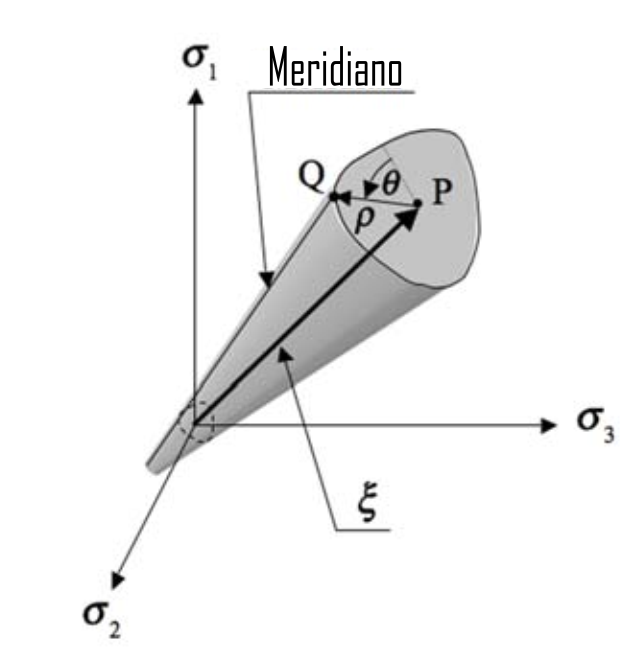
\includegraphics[width=0.5\linewidth]{images/Haigh_Wester.png}
    \label{fig:coordhaigh}
    \fonte{O autor (2020)}
\end{figure}

\section{O critério de escoamento}

O critério de escoamento pode ser representado através de uma função que pode ter como variáveis independentes os invariantes do tensor de tensões desviadoras, as coordenadas de haigh-Westergaard, os invariantes do tensor de tensões ou as tensões principais. \\

\subsection{Escoamento independente da pressão.}

 \cite{hill} mostrou que não há dependência da pressão na deformação plástica de materiais metálicos, portanto alguns critérios de deformação usam este tipo de abordagem. A afirmação anterior faz com que a função que descreve a superfície de escoamento tenha que ser dependente apenas de $J_2$ e $J_3$, já que $J_1$ é associado à pressão.

Um dos critérios de escoamento mais usados, e conhecido, é o critério de Von-Mises. Nele o autor do critério assume que a função de escoamento depende apenas de $ J_2 $. De acordo com \cite{hiermaier_2008} a superfície descrita por este critério forma um círculo no plano desviador, vide figura \ref{fig:trescamises}. Quando este círculo é projetado em algum plano das tensões principais, forma-se uma elipse. No espaço das tensões principais esta superfície pode ser descrita como um cilíndro, cujo centro é o eixo hidrostático, vide figura \ref{fig:suptrescaemises}.

\begin{figure}[H]
    \centering
    \caption{Superfície de escoamento de  von Mises e Tresca.}
    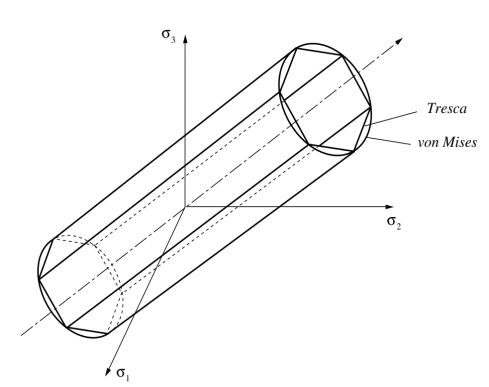
\includegraphics[width=0.7\linewidth]{images/Sup_trescaemises.png} % Do EA de souza Neto
    \label{fig:suptrescaemises}
    \fonte{\cite{neto_peric_owens_2008}}
\end{figure}

Outro critério muito conhecido é o de Tresca. Seu autor assume que a função que descreve a superfície de escoamento depende tanto de $ J_2 $ quanto de $ J_3 $. O terceiro invariante do tensor de tensões desviadoras, $ J_3 $, tem relação com a coordenada $ \theta $ de Haigh-Westergaard. Portanto, o estado de triaxialidade da tensão tem influência sob o escoamento neste critério. Em um plano desviador a superfície de escoamento de Tresca forma um hexaedro, vide figura \ref{fig:suptrescamises}, que coincide com a superfície de von-mises nos meridianos onde o ângulo $ \theta $ é múltiplo de $ 60º $. A menor distância entre o eixo hidrostático e a superfície de escoamento, no critério de Tresca, acontece nos ângulos múltiplos de $ 30º $ que significam estados de cisalhamento puro. A figura \ref{fig:trescamises} mostra a intersecção das superfícies de tresca e von Mises com um plano desviador qualquer.


\begin{figure}[H]
    \centering
    \caption{Projeção das superfícies de tresca e von Mises em um plano desviador.}
    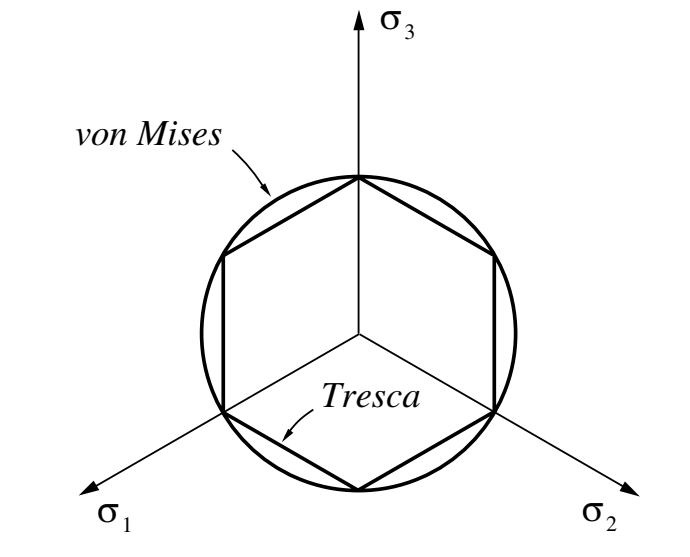
\includegraphics[width=0.7\linewidth]{images/trescaemises.png} % Do EA de souza Neto
    \label{fig:trescamises}
    \fonte{\cite{neto_peric_owens_2008}}
\end{figure}


\subsection{Escoamento dependente da pressão}

Apesar da pressão não influenciar o escoamento de materiais metálicos, ela deve ser levada em consideração quando outros materiais são simulados. Os critérios mais utilizados neste caso podem ser vistos como generalizações dos de Von-mises e de Tresca. A figura \ref{fig:mohrDrucker} mostra o critério de Mohr-Coulomb, que pode ser visto como uma generalização do critério de Tresca, e de Drucker-Prager, que generaliza o critério de Von-Mises.

\begin{figure}
    \centering
    \caption{Superfície de escoamento descrita pelos critérios de Mohr-Coulomb e Drucker-Prager}
    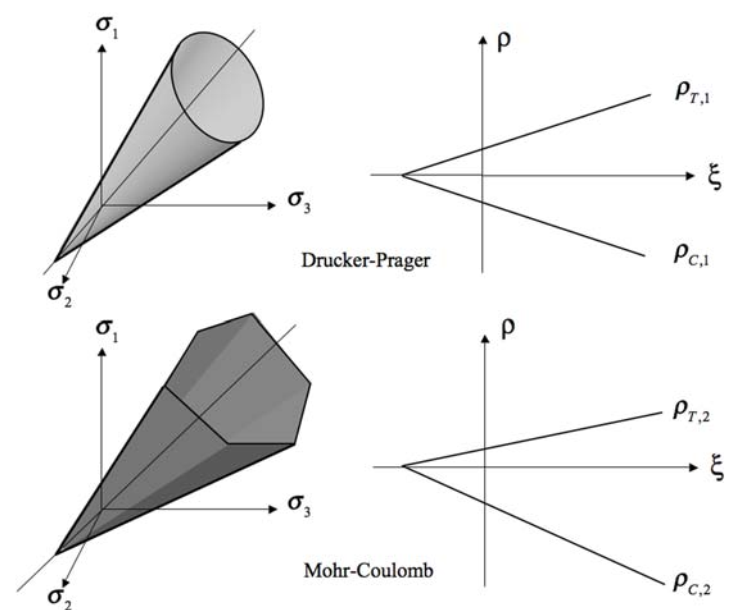
\includegraphics[width=0.7\linewidth]{images/tmohrdrucker.png}
    \label{fig:mohrDrucker}
     \fonte{\cite{neto_peric_owens_2008}}
\end{figure}

Tanto o critério de Mohr-Coulomb quanto o critério de Tresca apresentam descontinuidades na superfície de escoamento quando $\theta$ é multiplo de $ 60º $. Fato que, de acordo com  \cite{hiermaier_2008}, gera complicações numéricas quando algoritmos de retorno são usados para calcular a deformação plástica. Estes são os algorítmos mais usados quando um impacto balístico é simulado, sendo assim é apresentado um terceiro critério de falha na figura \ref{fig:Willamwarnke}, que é o de Willam-Warnke. A superfície descrita é suave para todos os ângulos $\theta$ facilitanto a aplicação de algoritmos de retorno. 

\begin{figure}
    \centering
    \caption{Superfície de escoamento descrita pelo critério de Willam-Warnke}
    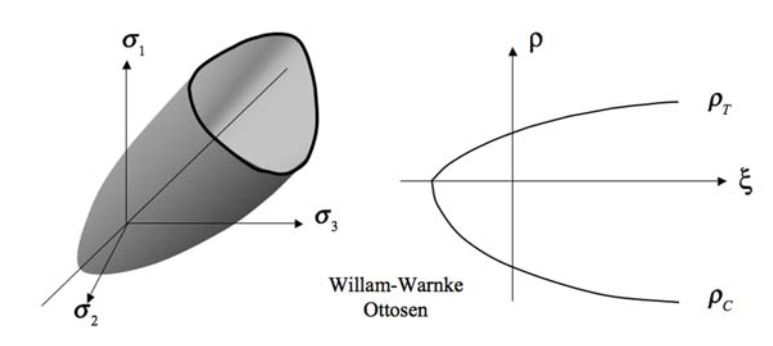
\includegraphics[width=0.7\linewidth]{images/willianwarnke.png} 
    \label{fig:Willamwarnke}
     \fonte{\cite{neto_peric_owens_2008}}
\end{figure}

\section{As funções de escoamento}

De acordo com \cite{neto_peric_owens_2008} a função de escoamento é responsável por aplicar o critério de escoamento usado. Inicialmente é imposto que a deformação plástica pode ocorrer apenas quando a função de escoamento $ \phi $ é nula.

\begin{equation}
     \phi(\boldsymbol{\sigma}, \boldsymbol{A}) = 0 
\end{equation}

Onde \gls{Cauchy} é o tensor de tensão de Cauchy, e $\boldsymbol{A}$ é um conjunto de variáveis termodinâmicas que estão ligadas ao encruamento.\\

De acordo com \cite{neto_peric_owens_2008} o seguinte conjunto, chamado domínio elástico é definido. 

\begin{equation}
    \mathcal{E} = \{ \gls{Cauchy} | \phi(\boldsymbol{\sigma}, \boldsymbol{A}) < 0   \}
\end{equation}

Em todo este conjunto as deformações plásticas não são permitidas. A visualização deste conjunto é auxiliada pelo espaço de tensões principais. Neste espaço o conjunto é formado pelos pontos onde a coordenada $\rho$ é menor do que a da superfície de escoamento. Note que a função de escoamento não restringe o tensor de tensões ao espaço principal, este é apenas um auxilio para o entendimento. As funções de escoamento são escritas levando em consideração o tensor descrito de forma geral, assim como a superfície de escoamento em seis dimensões.\\

O escoamento só pode ocorrer quando a tensão se localiza na superfície de escoamento, portanto esta é atingida quando a tensão faz parte do seguinte conjunto

\begin{equation}
    \mathcal{Y} = \{ \gls{Cauchy} | \phi(\boldsymbol{\sigma}, \boldsymbol{A}) = 0   \}
\end{equation}


\cite{neto_peric_owens_2008} apresenta a união destes dois conjuntos. Esta união forma um novo conjunto, chamado de tensões plasticamente admissíveis ou simplesmente tensões admissíveis.

\begin{equation}
    \overline{\mathcal{E}} = \{ \gls{Cauchy} | \phi(\boldsymbol{\sigma}, \boldsymbol{A}) \leq 0   \}
\end{equation}

No conjunto de tensões admissíveis estão todas as tensões que o material pode assumir em qualquer momento. Sendo assim, tensões com coordenada $\rho$ superiores à da tensão de escoamento são inadmissíveis. \par

Além da função de escoamento é necessário definir uma expressão para o fluxo do material quando este está deformando plasticamente. A lei de fluxo é responsável tanto pela taxa de deformação quanto por sua direção.

\begin{equation}
    \dot{\varepsilon}^p = \dot{\gamma} \boldsymbol{N}
\end{equation}

Onde \gls{gamma} é chamado de multiplicador plástico, ele define a magnitude da taxa de variação da deformação plástica.  \gls{N} é o vetor fluxo plástico. Este é um vetor é unitário, normal à superfície de escoamento e é definido da seguinte forma

\begin{equation}
    \boldsymbol{N} = \frac{\partial \boldsymbol{\Psi}}{\partial \boldsymbol{\sigma}} = \frac{\partial \boldsymbol{\phi}}{\partial \boldsymbol{\sigma}}
\end{equation}

Onde $\boldsymbol{\Psi} = \boldsymbol{\Psi}(\boldsymbol{\sigma}, \boldsymbol{A}) $ é o chamado potencial de fluxo. Porém assume-se, neste trabalho, que todos os modelos são associativos, portanto $ \boldsymbol{\Psi} = \boldsymbol{\phi} $. O vetor de Prandt-Reuss é o vetor de fluxo plástico aplicado à superfície de von-mises. No espaço das tensões principais ele tem direção normal ao círculo formado pela superfície em um plano desviador.

\section{As funções de encruamento}

As funções de encruamento são responsáveis por relacionar a tensão de escoamento às variáveis de estado relevantes. Alguns exemplos de variáveis de estado que podem ser consideradas são: A deformação plástica acumulada $ \overline{\varepsilon}^p $, a taxa de deformação $ \dot{\varepsilon} $ e a temperatura $ T $. A escolha das variáveis envolvidas depende do uso pretendido e da abordagem de um determinado grupo de pesquisa. Existem tanto modelos micromecânicos que levam em consideração a estrutura do , quanto modelos fenomenológicos que levam apenas a resposta macroscópica em consideração. Para apresentar funções de encruamento é interessante que se tenha em vista a função de escoamento na qual o encruamento é aplicado, dado que a tarefa da função de encruamento é alterar as características da superfície de escoamento. A formulação de von-mises será usada para apresentar as funções de encruamento pertinentes ao âmbito de impacto balístico já que ela é simples e de fato é base para muitos modelos. \\

A função de escoamento de von-mises assume que a deformação plástica ocorre quando o invariante $ J_2 $ assume um valor crítico.
\begin{equation} \label{eq:vonesc}
    \boldsymbol{\phi}(\boldsymbol{\sigma}) = \sqrt{J_2} - \tau_y
\end{equation}

Onde $ \tau_y $ é a tensão de escoamento inicial em cisalhamento. Ela se relaciona com a tensão de escoamento em tração uniaxial da seguinte forma.
\begin{equation}
    \sigma_y = \sqrt{3}\tau_y
\end{equation}

De acordo com \cite{neto_peric_owens_2008} usando esta relação e sabendo que 
$ J_2 = \frac{1}{3}\boldsymbol{\sigma}^2 $
é possível escrever a função de escoamento de von-mises da seguinte forma,

\begin{equation} \label{eq:vonesc}
    \boldsymbol{\phi}(\boldsymbol{\sigma}) = q(\boldsymbol{\sigma}) - \sigma_y = \sqrt{3 J_2} - \sigma_y
\end{equation}

 A função  $ q(\sigma) $ é amplamente conhecida como tensão de von-mises ou tensão equivalente. Portanto, de acordo com a função de escoamento de Von-Mises o escoamento ocorre quando a tensão equivalente é igual à tensão de escoamento naquele ponto.
 
 \subsection{Modelo da plasticidade isotrópica ou cinemática}

De acordo com \cite{rao_narayanamurthy_simha_2016} a expressão da tensão de von mises em uma dimensão para este modelo é a seguinte 

\begin{equation}
    \sigma_y = \left[1 + (\frac{\dot{\varepsilon}}{C})^{(\frac{1}{P})} \right](\sigma_0 + \beta E^p \overline{\varepsilon}^p)
\end{equation}

Este é baseado nos modos clássicos de plasticidade citados anteriormente. Nele $ \beta $ é chamado de parâmetro de endurecimento. Quando $ \beta = 0 $ o encruamento é completamente cinemático, caso $ \beta = 1 $ é completamente isotrópico, sendo permitidos valores de $ \beta $ entre $0$ e $1$. $ E^p $ é o módulo tangente ou o coeficiente de encruamento plástico, de acordo com \cite{neto_peric_owens_2008} quando generalizado para três dimensões
este se torna um tensor de quarta ordem. Já $\gls{defplastacu}$ é a deformação plástica acumulada, que pode ser calculada de acordo com a equação \ref{eq:defplastacu}. $ \sigma_0 $ é a tensão de escoamento inicial, $\dot{\varepsilon} $ é a taxa de deformação. Finalmente $ C $ e $ P $ são parâmetros da taxa de deformação de Cowper-Symonds. \par 

\begin{equation} \label{eq:defplastacu}
    \overline{\varepsilon}^p = \int_0^t |\dot{\varepsilon}^p| dt
\end{equation}

De acordo com \cite{rao_narayanamurthy_simha_2016} este tipo de modelo é o mais simples em termos da obtenção dos parâmetros necessários para uma simulação de impacto balístico, já que é de origem estática. Ele é aplicável a situações onde a velocidade do impacto é baixa e os efeitos térmicos podem ser ignorados. \cite{rao_narayanamurthy_simha_2016} afirma também que este modelo serve para prever satisfatoriamente
 parâmetros como a velocidade residual, profundidade de penetração e padrões de deformação.
 
 %CONTINUAR REVISAO
 \subsection{Modelo de Johnson-Cook}
 
 O modelo de Johnson-Cook é um modelo empírico que data de 1983 e é o mais usado quando o comportamento de metais em regimes dinâmicos é simulado. Ele leva em consideração os efeitos tanto da taxa de deformação quanto da temperatura na tensão de escoamento. A expressão da tensão equivalente, em uma dimensão, para este modelo é a seguinte
 
 \begin{equation}
     \sigma_y = [A + B (\overline{\varepsilon}^p)^n][1 + C ln(\dot{\varepsilon}^*)][1-(T^*)^m]
\end{equation}
 na qual 
\begin{align}
     \dot{\varepsilon}^* = \frac{\dot{\overline{\varepsilon}}^p}{\dot{\varepsilon}} &&
     T^* = \frac{T-T_r}{T_m-T_r}
 \end{align}
 
 $A$ é a tensão inicial de escoamento, $ B $ é o coeficiente de encruamento e $ n $ é o expoente de encruamento, $ \overline{\varepsilon}^p $ é a deformação plástica acumulada,  $\dot{ \overline{\varepsilon}^p} $  é a taxa da deformação plástica acumulada, $ \dot{\varepsilon}_0 $ é a taxa de deformação de referência e C é o coeficiente da taxa de deformação. Veja que $ T_m $ é a temperatura de fusão e $ T_r $ 
é a temperatura de referência, normalmente $ 298 \, K $ e $ m $ é o expoente térmico. \\

O primeiro termo entre colchetes relaciona a resistência dinâmica do material com o encruamento. De acordo com \cite{Crouch} o encruamento é o aumento da resistência do material devido a interação de discordâncias entre si e com barreiras externas. O empilhamento de discordâncias no contorno de grão ou em fases secundárias gera uma tensão contrária à aplicada e acaba aumentando a 
resistência do material à deformação. \\

O segundo termo entre colchetes é relacionado com a sensibilidade da resistência do material a diferentes taxas de deformação. \cite{Crouch} cita uma série de estudos que evidenciam a sensibilidade dos metais à taxa de deformação. Na fig \ref{fig:taxadef} é apresentado o efeito da taxa de deformação em alguns deles.

\begin{figure}[H]
    \centering
    \caption{Efeito da taxa de deformação na tensão de escoamento e na tensão máxima suportada de alguns aços.}
    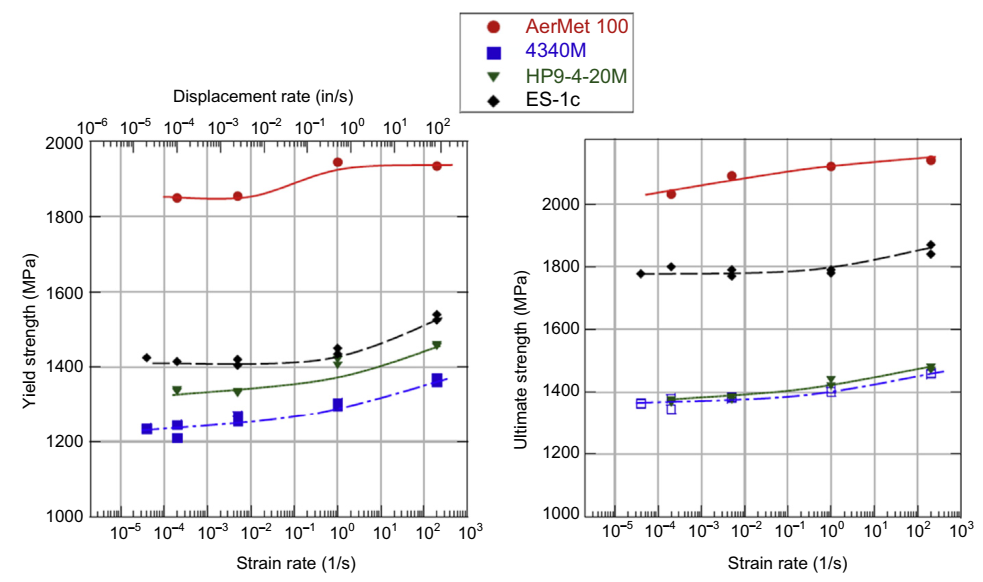
\includegraphics[width=0.5\linewidth]{images/strainrateeffect.png} 
    \label{fig:taxadef}
    \fonte{\cite{Crouch}}
\end{figure}

O terceiro termo tem relação com a temperatura, portanto ele diz respeito a diminuição da resistência do material devida ao aumento da temperatura. De acordo com \cite{Crouch} assume-se que o acréscimo de temperatura ocorre de forma adiabática e a fórmula para o cálculo do aumento da temperatura é a que segue

\begin{equation}
    \Delta T = \int_0^{\overline{\varepsilon}} \mathcal{X} \frac{\sigma_{eq}}{\rho C_p} d\overline{\varepsilon}
\end{equation}

Aqui o símbolo $ \mathcal{X}$ é novamente utilizado porém com outro sentido, algo não recomendado mas necessário para manter a identificação dos símbolos encontrados em diferentes literaturas. Neste caso $ \mathcal{X} $ é o coeficiente de Taylor-Quinney que em geral é 0.9.\footnote{Antes o símbolo $\mathcal{X}$ significava a função movimento, no contexto da cinemática.} $C_p$ é o calor específico do material, $ \rho $ a densidade, $ \sigma $ a tensão equivalente de von-mises e $ \varepsilon$ a deformação. 

\subsection{Modelo de dano de Johnson-Cook}

O modelo de dano de Johnson-Cook não é uma lei de encruamento, porém sua inserção neste tópico foi julgada adequada por conta de sua relação com o modelo de mesmo nome.
Este modelo de dano, também chamado critério de dano de Johnson-Cook, insere uma nova variável de estado chamada Dano. O dano no material varia de $ 0 $ a $ 1 $. A expressão usada para calcular o dano por este critério é a que segue

\begin{equation} \label{eq:danoincrJC}
    D = \sum \frac{\Delta \overline{\varepsilon}^p}{\varepsilon_f}
\end{equation}

Sendo $ \overline{\varepsilon}^p $ novamente a deformação plástica acumulada e $ \varepsilon_f $ a deformação de falha, calculada da seguinte forma

\begin{equation}
    \varepsilon_f = (D_1 + D_2 exp(D_3 \sigma^*))(1 + D_4 ln(\dot{\varepsilon}^*))(1 + D_5 T^*)
\end{equation}

De acordo com \cite{Crouch} o primeiro termo entre parenteses tem relação com a triaxialidade da tensão, o segundo toma conta do decréscimo da deformação de falha com o aumento da taxa de deformação e o terceiro relaciona o aumento da deformação de falha com o aumento da temperatura. \\

A expressão \ref{eq:danoincrJC} é a mais utilizada na literatura, porém está descrita de forma incremental. Esta é a forma usada para a implementação computacional dos modelos, mas ela não será abordada neste trabalho. A forma continua da mesma expressão é a que segue.

\begin{equation}
    D = \frac{\overline{\varepsilon}^p}{\varepsilon_f}
\end{equation}

Na qual a deformação plástica acumulada é calculada de acordo com \ref{eq:defplastacu}.

O critério de dano de Johnson-Cook é o mais usado para metais e normalmente a função de encruamento que leva o mesmo nome é complementada por este critério. Apesar disto nada impede o acoplamento deste critério com outras funções de encruamento. A consequência da falha no material pode ser lida de diversas formas e normalmente os códigos de propagação de onda apresentam opções para diferentes abordagens. Um elemento que falhou completamente, ou seja com $ D = 1  $, pode ser tanto retirado da simulação, por meio do mecanismo de erosão, quanto mantido suportando apenas tensões compressivas. Um dos usos para o dano é a redução da resistência ao escoamento, neste caso ele é tratado como uma variável interna.

\subsection{Modelo de Zerilli-Armstrong}
 
 Este modelo, diferente do modelo de Johnson-Cook, leva em consideração a estrutura cristalina do material. Ele existe em duas versões. A primeira é válida para materiais que assumem a estrutura cúbica de face centrada, CFC, e segue a expressão \ref{eq:ZA1}. A segunda vale para materiais constituídos pela estrutura cubica de corpo centrado, CCC, que é apresentada em \ref{eq:ZA2}. \\
 
 \begin{equation} \label{eq:ZA1}
     \sigma_y = C_0 + C_1 exp[-C_3T + C_4Tln(\dot{\overline{\varepsilon}}^p)] + C_5 (\overline{\varepsilon}^p)^n
 \end{equation}
 
  \begin{equation} \label{eq:ZA2}
     \sigma_y = C_0 + C_2\sqrt{\overline{\varepsilon}^p}exp[-C_3T + C_4Tln(\dot{\varepsilon}^p)] 
 \end{equation}
 
Onde $C_0$,$C_1$,$C_2$,$C_3$,$C_4$ são parâmetros de ajuste, $ C_5 $ é o coeficiente de encruamento e n é o expoente de encruamento. \\

O que motiva a apresentação de modelos diferentes de acordo com a estrutura cristalina dos metais é a diferença entre os mecanismos que coordenam a deformação plástica para diferentes estruturas cristalinas.
 
 \subsection{Modelos de Johnson-Holmquist}
 
 Os modelos de Johnson-Holmquist são os mais usados para simular o comportamento de cerâmicos durante um impacto em alta velocidade. Existem três versões deste modelo, porém as mais usadas são a primeira e a segunda. A terceira versão não será apresentada, ela é uma relaeitura da primeira versão. O primeiro modelo de Johnson-Holmquist é também chamado de JH-1, consequentemente o segundo é o JH-2.  \\
 
 Todos os três modelos descrevem a tensão equivalente como dependente da pressão. Uma interpretação possível é que a superfície de escoamento para estes modelos se assemelha com a de Drucker-Prager, porém para afirmar categoricamente como de fato é a superfície é necessário ter acesso à implementação dos modelos. O relatório \cite{JH2Imp} fala sobre a implemetação do segundo modelo de Johnson-Holmquist,
 porém trata $ \dot{\varepsilon}^p $ como um valor já disponível. Como dito anteriormente este valor é dependente de um mutiplicador e de um vetor de fluxo plástico, sendo assim ele não está naturalmente disponível e deve ser calculado. Duas são as possibilidades para o motivo de assumir este valor como dado. \\
 
 A primeira possibilidade é assumir que como o autor do relatório usa nomes compatíveis com a teoria de von-miese, ele chama a tensão de equivalente e a deformação de equivalente, subentende-se que o critério de von-mises é usado e portanto não seria errado inferir que o vetor de fluxo é o de Prandt-Reuss. Sendo assim o autor do relatório não quis se prolongar em tal discussão e tomou a informação como dada. \\
 
 A possibilidade alternativa 
 é que a implementação deste vetor possa estar protegida por um segredo industrial e fica de fato dúbio qual vetor de fluxo é usado. Esta dificuldade se repete para todos os modelos de Johnson-Holmquist, ao menos na porção da literatura pesquisada. A segunda possibilidade é corroborada por uma discussão no site acadêmico Researchgate.\footnote{ O sitio onde está a pergunta e posterior discussão é  \url{https://www.researchgate.net/post/How_can_I_implement_JH-2Johnson_holmquist_constitutive_equation_in_explicit_FEM} } Nesta um pesquisador solicita ajuda para implementar o segundo modelo de Johnson-Holmquist pois não consegue calcular corretamente $ \dot{\varepsilon}^p $ gerando erros em seus resultados. Julgando que a falta desta informação não prejudica a simples apresentações dos modelos que aqui será feita. O primeiro modelo de Johnson-Holmquist é apresentado a seguir. \\
 
 \subsubsection{O primeiro modelo de Johnson-Holmquist}
 
O primeiro modelo de de Johnson-Holmquist usa uma descrição polinomial por partes da tensão equivalente. De acordo com \cite{holmquist_johnson_2002} a resistência inicial do material intacto $ \sigma_0 $ é representada por uma função formada por segmentos de reta que é ajustada de acordo com o material. Esta função é representada pela linha contínua superior da figura \ref{fig:JH1Tensao}. Esta resistência é relacionada a uma taxa de deformação adimensional
\begin{equation}
    \dot{\varepsilon}^* = \dot{\varepsilon}/\dot{\varepsilon_0}
\end{equation}
onde $ \dot{\varepsilon_0} $ 
é a taxa de deformação de referência e é normalmente equivalente a $1.0 s^{-1} $. Quando $ \dot{\varepsilon}^* = 1.0 $ a resistência do material é $ \sigma_0 $. Para taxas diferentes de deformação adimensional é aplicada expressão \ref{eq:JH1tensao}, onde $ C $ é chamada constante da taxa de deformação e tem relação com a sensibilidade do material à velocidade de solicitação. 

\begin{equation} \label{eq:JH1tensao}
    \sigma_y = \sigma_0(1.0 + C ln\dot{\varepsilon}^*)  
\end{equation}

\begin{figure}[H] 
    \centering
    \caption{Relação entre a tensão de von-mises e a Pressão para o primeiro modelo de Johnson-Holmquist}
    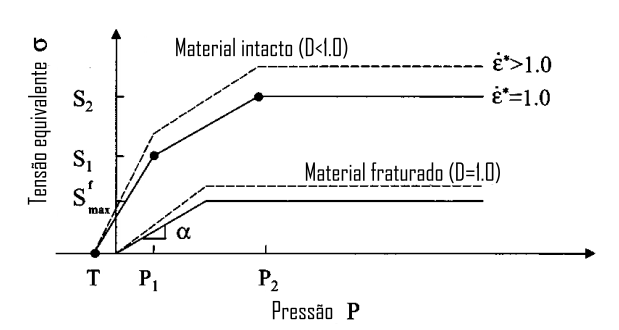
\includegraphics[width = 0.7\linewidth]{images/sigmapressao.png} 
    \label{fig:JH1Tensao}
    \fonte{\cite{holmquist_johnson_2002}}
\end{figure}


A expressão \ref{eq:JH1tensao} é responsável por descrever a resistência do material intacto, por intacto entende-se que o dano $ D \neq 1 $. Diferente de todos os modelos vistos até agora a resistência do material depende do dano, assim há outra curva que descreve a resistência do material que falhou. O modelo de dano é acoplado à função de encruamento, consequntemente é apresentado a seguir. 
O dano é calculado de forma semelhante ao de Johnson-Cook. O cálculo é novamente apresentado da forma incremental. 

\begin{equation} \label{eq:danoJH}
    D = \sum \frac{\Delta \overline{\varepsilon^p} }{\varepsilon^p_f}
\end{equation}

A Diferença entre as duas é o termo $ \varepsilon^p_f $ que é chamado deformação de falha e é calculado através da seguinte expressão

\begin{equation}
    \varepsilon^p_f = \phi(P_3 + T)
\end{equation}

Onde $ P_3 $ é a pressão em que ocorre a saturação da deformação de falha, que pode ser vista na figura \ref{fig:deffalhapressJH1}. $ T $ é a tensão hidrostática trativa máxima, na qual a deformação de falha é nula e quando atingida o material falha instantaneamente. Esta tensão está representada na figura \ref{fig:JH1Tensao} pela letra $T$. $ \phi $ é o coeficiente angular da reta descrita pela deformação de falha antes da saturação, calculado da seguinte maneira

\begin{equation}
    \phi = \ddfrac{\varepsilon^{max}_{f}}{(P_3 + T)}
\end{equation}

\begin{figure}
    \centering  
    \caption{Relação da deformação de falha com a pressão}
    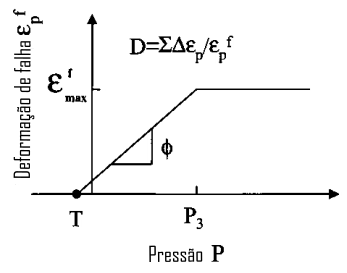
\includegraphics[width = 0.7\linewidth]{images/deffalhapressao.png} 
    \label{fig:deffalhapressJH1}
    \fonte{\cite{holmquist_johnson_2002}}
\end{figure}

Na figura \ref{fig:JH1Tensao} também está presente a descrição da resistência do material que atingiu a condição de falha, ou seja $ D = 1 $. Esta resistência é descrita usando dois parâmetros do modelo, que são particularmente difíceis de se obter usando experimentação. Devido a dificuldade de obtenção experimental, a definição destes é feita através da calibração da simulação de um teste balístico. \cite{holmquist_johnson_2002} aponta que tal característica do modelo não é desejável, porém a simulação do material sem estes dois patamares de força leva a resultados insatisfatórios.
Os parâmetros citados são $ \alpha $ que é o coeficiente angular da reta que representa a resistência do material que falhou até atingir $ S^{max}_f $, que é a resistência máxima do material falhado. \par

Este modelo apresenta outra particularidade, que é o acoplamento de uma  equação de estado. A pressão no material é caracterizada pela seguinte expressão 

\begin{equation} \label{eq:JHEOS}
    P = K_1 \mu + K_2 \mu^2 + K_3 \mu^3
\end{equation}

\begin{figure} \label{fig:pressvsdefvolJH1}
    \centering
    \caption{Relação entre a pressão e a deformação volumétrica} 
    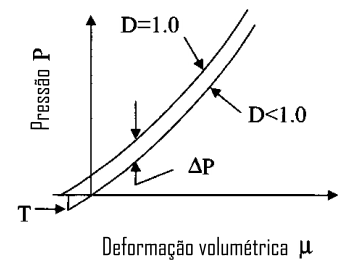
\includegraphics[width=0.7\linewidth]{images/defvolpressao.png}
    \label{fig:my_label}
    \fonte{\cite{holmquist_johnson_2002}}
\end{figure}

Na qual $ \mu $ representa a deformação volumétrica do corpo e é calculada da seguinte maneira

\begin{equation}
    \mu = \frac{V_r}{V} - 1 = \frac{\rho}{\rho_r} - 1
\end{equation}

Onde $ K_1 $, $ K_2 $ e $ K_3 $ são constantes. $ K_1 $ é o módulo volumétrico do material, já as outras não tem leitura física definida. Para pressões negativas, ou tensões hidrostáticas trativas, a expressão  \ref{eq:JHEOS} é substituída por $ P = K_1 \mu $. \\


De acordo com \cite{holmquist_johnson_2002}
quando o material falha o modelo permite que haja um acréscimo $ \Delta P $ na pressão, de forma que 

\begin{equation} \label{eq:EOSJH2}
	P = K_1 \mu + K_2 \mu^2 + K_3 \mu^3 + \Delta P
\end{equation}


Este acréscimo de pressão é decorrente da redução da energia elástica interna  do material que se deve ao decréscimo das tensões desviadoras no local. A expressão da energia elástica interna no material é a seguinte

\begin{equation}
	e_{el} = \ddfrac{\sigma_{eq}^2}{6G}
\end{equation}

Na qual $ G $ é o módulo de cisalhamento. \\

Novamente de acordo com \cite{holmquist_johnson_2002}

a  energia elástica perdida pode ser transformada em energia potencial hidrostática, que se apresenta no termo adicional $ \Delta P $ da expressão \ref{eq:EOSJH2}. A expressão para calcular $\Delta P$ é a seguinte

\begin{equation} \label{eq:JHEOSDeltaP}
	\Delta P = -K_1 \mu_f + \sqrt{(K_1 \mu_f)^2 + 2 \beta K_1 \Delta e_{el}}
\end{equation} 

Onde $ \mu_f $ é a deformação volumétrica no momento da falha. O termo $ \beta $ é uma constante do material, de forma que se $ \beta = 0 $, então $ \Delta P = 0 $ e nenhuma energia elástica interna é transformada em potencial hidrostática. Se $ \beta = 1 $ toda energia elástica perdida é alocada e $ \Delta P $ tem seu valor máximo. \\


As figuras \ref{fig:JH1Tensao}, \ref{fig:deffalhapressJH1} e \ref{fig:pressvsdefvolJH1} são bons resumos do primeiro modelo de Johnson-Holmquist. Mesmo se tratando do primeiro modelo ele ainda é muito usado por obter bons resultados e ser simples. Uma característica importante dele é que não permite redução da resistência do material com o aumento do dano, o que ocorre é uma redução abrupta quando o dano atinge o valor crítico $ D = 1 $. Por conta disto este modelo é usado nos materiais que apresentam tal caracterísica como por exemplo o carbeto de silício. Defirente do JH-1 o modelo JH-2 apresentado a seguir permite que a resistência do material diminua ao longo do processo de danificação. \par

\subsubsection{O segundo modelo de Johnson-Holmquist}

Como foi dito anteriormente o segundo modelo de Johnson-Holmquist permite a redução da resistência do material a medida que este é danificado, este comportamento pode ser visto na figura \ref{fig:JH2tensao}. Este modelo usa uma normalização de seus parâmetros que usa dados do limite elástico de Hugoniot. O limite elástico de Hugoniot será explicado no próximo capítulo mas é basicamente a tensão a partir da qual o material começa a se deformar plasticamente em um ensaio uniaxial de deformação.

As tensões neste modelo são todas normalizadas da seguinte forma $ \sigma^* = \sigma/\sigma_{LEH} $ onde $ \sigma_{LEH} $ é a tensão no limite elástico de Hugoniot ou LEH. $ \sigma $ é a tensão equivalente, que segue a seguinte expressão

\begin{equation} \label{eq:JH2tensao}
    \sigma^* = \sigma^*_i - D(\sigma^*_i - \sigma^*_f)
\end{equation}

Na qual $ \sigma^*_i $ é a resistência inicial normalizada e $ \sigma^*_f $ é a resistência normalizada do material fraturado. Estas duas podem ser respectivamente calculadas de acordo com as expressões \ref{eq:tensaoinicialJH2} e \ref{eq:tensaofraturadaJH2}.

\begin{equation} \label{eq:tensaoinicialJH2}
    \sigma^*_i = A(P^* + T^*)^N (1 + C ln\dot{\varepsilon}^*)
\end{equation}

\begin{equation}
    \sigma^*_f = B(P^*)^M(1 + Cln\dot{\varepsilon}^*)
\end{equation}

Nas quais $A$, $B$, $C$, $M$ e $N$ são constantes do material. Em  \cite{johnson_holmquist_1994} o autor do modelo cita que é possível limitar $ \sigma^*_f $, de modo que este fique menor ou igual a $ S^{max}_f $ que novamente é a resistência máxima do material pós falha. O autor não fala nada sobre a tensão pós falha ser ou não normalizada, mas levando em consideração que o modelo é todo normalizado seria prudente usar $ (S^{max}_f)^*$. 
A taxa de deformação normalizada $ \dot{\varepsilon}^* $ tem o mesmo significado e é calculada da mesma forma que no primeiro modelo. $ P^* $ é a pressão normalizada, sendo \begin{equation}
    P^* = P/ P_{LEH} 
\end{equation}  

$ T^* $ é a tensão hidrostática trativa máxima normalizada, calculada da seguinte maneira \begin{equation}
    T^* = T/P_{LEH} 
\end{equation}   
\begin{figure}
    \centering
    \caption{Tensão equivalente normalizada no segundo modelo de Johnson-Holmquist}
    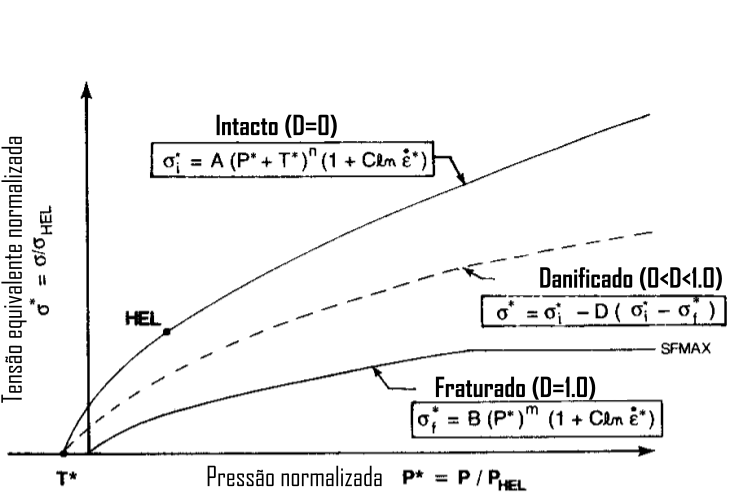
\includegraphics[width=0.7\linewidth]{images/sigmapressaoJH2.png}
    \label{fig:JH2tensao}
    \fonte{\cite{johnson_holmquist_1994} traduzida pelo autor.}
\end{figure}

O segundo modelo de Johnson-Holmquist calcula o dano seguindo a expressão \ref{eq:danoJH}, que é a mesma do primeiro modelo, porém a deformação de falha $ \varepsilon^p_f $ agora é calculada da seguinte maneira

\begin{equation}
    \varepsilon^p_f = D_1(P^* + T^*)D^2
\end{equation}

Onde $ D_1 $ e $ D_2 $ são constantes do material % TODO: Verificar como estas CTES são calculadas, se n é por calibração
e novamente quando a tensão hidrostática ou pressão no material é trativa e igual a $ -T^* $ o material não é capaz de suportar qualquer deformação e falha de forma instantânea. O comportamento da deformação de falha é apresentado na figura \ref{fig:danoJH2}.

\begin{figure}
    \centering
    \caption{Comportamento da deformação de falha equivalente.}
    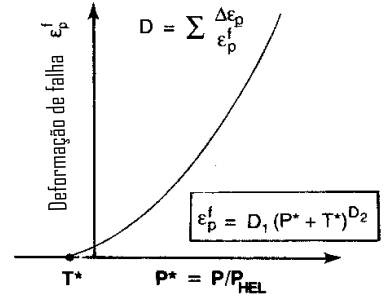
\includegraphics[width=0.7\linewidth]{images/deffalhaJH2.png} 
    \label{fig:danoJH2}
    \fonte{\cite{johnson_holmquist_1994} traduzida pelo autor.}
\end{figure}

Novamente o modelo apresenta uma equação de estado acoplada, que segue a expressão \ref{eq:JHEOS}. Neste caso o acréscimo da pressão acontece de forma gradual, já que o material vai perdendo resistência ao longo do processo de danificação. A expressão corrigida é idêntica, vide eq. \ref{eq:EOSJH2}. O autor apresenta $ \Delta P $ de forma incremental no artigo de apresentação do modelo, \cite{johnson_holmquist_1994} . Porém como a formulação incremental não será abordada, a equação \ref{eq:JHEOSDeltaP} permanece válida e pequenas parcelas de energia são transformadas em cada ciclo. 


 
 
 
 
 
 
 
 
 







\chapter{A mecânica da penetração}

A balística terminal trata da última parte do processo balístico, na qual acontece o impacto entre o projétil e o anteparo. A palavra armadura será usada neste capítulo como referente à composição entre as camadas de proteção, de modo que ela se refere à composição, que pode contar com uma ou mais placas e estruturas de materiais diversos. O anteparo é a primeira camada, logo recebe o contato inicial. Existem duas classes gerais quando se fala em armadura, as passivas e as reativas. As reativas são aquelas nas quais a energia cinética do projétil é usada para disparar alguma medida de reação. O projétil pode, por exemplo, causar uma pequena explosão que gera uma onda na direção contrária ao deslocamento dele. A explosão pode destruí-lo ou mudar sua direção. \\

Neste capítulo o foco será em armaduras passivas. Nelas a energia do projétil não é usada e é função dos materiais presentes na armadura diminuí-la. O sistema desejável é leve e ao mesmo tempo resistente, porém este não é um feito simples. A simulação por elementos finitos usando algoritmos complexos de plasticidade, aplicados a casos envolvendo  deformações severas, são necessários para o estudo deste tipo de sistema. Muitas das conclusões clássicas advém da aplicação deste tipo de simulação. \\
Historicamente é dominante o uso de chapas maciças de aço na qual a armadura é o anteparo, não havendo uma composição com diferentes materiais e funções. O uso de chapas monolíticas de aço não apresenta problemas quanto à absorção de energia e constituem ótimas blindagens, quando as características mecânicas apropriadas estão presentes. Dentre as características m necessárias, a mais importante de acordo com \cite{Crouch} é a dureza, porém mesmo aços com dureza e microestrutura adequada necessitam de grandes espessuras quando expostos a um impacto em altas velocidades. \\

Um exemplo histórico disso é a tentativa de construção de um veículo chamado Panzerkampfwagen VIII Maus, pela Alemanha durante a segunda guerra mundial. Este veículo contaria com chapas de aço de 240 mm de espessura, todavia este tipo de chapa seja suficiente para absorver a energia de qualquer projétil da época. Sua fabricação devia ser extremamente dificultosa, \cite{Crouch} reporta que até hoje fazer uma chapa muito espessa ter as propriedades corretas ao longo de sua espessura é um desafio. O item crítico para a falha do projeto foi que nenhum sistema de motorização e transmissão da época conseguiria propelir suficientemente o veículo. Atravessa-lo por uma ponte também não seria possível por conta de sua enorme massa.  \\

 Em geral a absorção de energia e a massa possuem uma relação inversamente proporcional. Ao longo dos anos processos de fabricação avançados e novos materiais surgiram e se desenvolveram para aumentar a proteção oferecida por sistemas mais leves. Um grupo de materiais muito presente neste avanço é o de cerâmicos. Um dos grandes projetos nesta área foi patrocinado por uma organização americana chamada DARPA.\footnote{Darpa em inglês significa Defense Advanced Research Projects Agency, ou em português agência de projetos avançados de pesquisa em defesa} Este projeto, chamado programa de armaduras leves, fomentou a criação do primeiro modelo computacional para a simulação de armaduras cerâmicas. Este programa foi amplamente usado para gerar avanços no entendimento deste tipo de material, em situações de impacto balístico. Alguns relatórios originados destes estudos estão disponíveis de forma aberta, por exemplo \cite{firstreport}. Este capítulo busca revisar aspectos da mecânica da penetração que são pertinentes à armaduras compostas pela composição entre cerâmicas e metais. \\
 
  \section{O comportamento dinâmico}
 
 Em relação a taxas quasi-estáticas os materiais submetidos a altas taxas de deformação apresentam propriedades mecânicas diferentes. De acordo com \cite{Hazell} a resistência de forma geral costuma aumentar, metais tendem a ficar mais resistentes porém menos dúcteis, sem haver alteração na rigidez. O mecanismo deste tipo de alteração em metais pode ser explicado, de acordo com \cite{Hazell}, pelo impedimento da movimentação de discordâncias durante a deformação plástica.\\ 
 
 Tanto para cerâmicos quanto para metais a resistência é, na maioria dos casos, proporcional à taxa de deformação
 \begin{equation}
 	\boldsymbol{\sigma} \propto \dot{\boldsymbol{\varepsilon}}
 \end{equation}
 
onde $ \dot{\boldsymbol{\varepsilon}} $ é a taxa de deformação e sua unidade é $ s^{-1} $.\\
Durante uma deformação inelástica há severa transformação de trabalho em calor, logo a temperatura na região de deformação sobe vertiginosamente. Metais acabam por sofrer, em vários casos, redução da resistência por conta de altas temperaturas. Esta redução é mais difícil em materiais cerâmicos por conta de suas altas temperaturas de fusão, costumeiras neste tipo de material. Observe que isto se reflete nos modelos mais usados para cada material, que foram revisados no capítulo  \ref{Cap: ModConst}. O modelo mais usado em metais é o de Johnson-Cook e tem um termo que trata especificamente da sensibilidade da resistência à temperatura. Para cerâmicas, nos modelos mais usados, que sãos os de Johnson-Holmquist, não há menção direta à temperatura. \\ 

O processo de penetração pode ser classificado como adiabático por conta do pouco tempo para a dissipação do calor gerado. Como visto anteriormente, isto pode gerar zonas de enfraquecimento térmico severo em materiais suscetíveis, pois o calor fica concentrado em regiões pequenas. Outra variável termodinâmica que tem influência no processo é a pressão. Se antes os metais se prejudicavam com o aumento da temperatura agora as cerâmicas, em geral, são beneficiadas pelo aumento da pressão. Inclusive \cite{Hazell} cita que há grupos que sugerem que a pressão tem influência positiva maior sob a resistência ao escoamento do que a própria taxa de deformação.
Um ponto importante é o comportamento do material cerâmico pós falha, tanto \cite{Hazell} quando \cite{holmquist_johnson_2002} citam a dificuldade de mensurar a resistência do material pós falha. É conhecido que a pressão tem influência na resistência do material que falhou, \cite{holmquist_johnson_2002} discute brevemente tal ponto. Algumas técnicas de simulação avançadas permitem substituir o elemento que sofreu erosão por uma partícula livre fazendo com que a pressão não diminua no local, \cite{johnson_2011} comenta tais técnicas.\\

\section{Os modos de falha}

Quando se estuda a proteção é primordial conhecer o ofensor. Uma munição completa é apresentada na figura \ref{fig:projetilinteiro}. O funcionamento parte da explosão da espoleta (Primer), então o propulsor (Propellant) propele o projétil (Bullet).\\
\begin{figure}[H]
	\centering
	\caption{Munição de armas pequenas. (Para correção: Aqui tenho um problema com a nomenclatura. Traduzi small arms para armas pequenas, mas deve ter algum nome mais correto. E não traduzi a imagem pois não achei algo bem defindo, então preferi apresentar em inglês.)}
	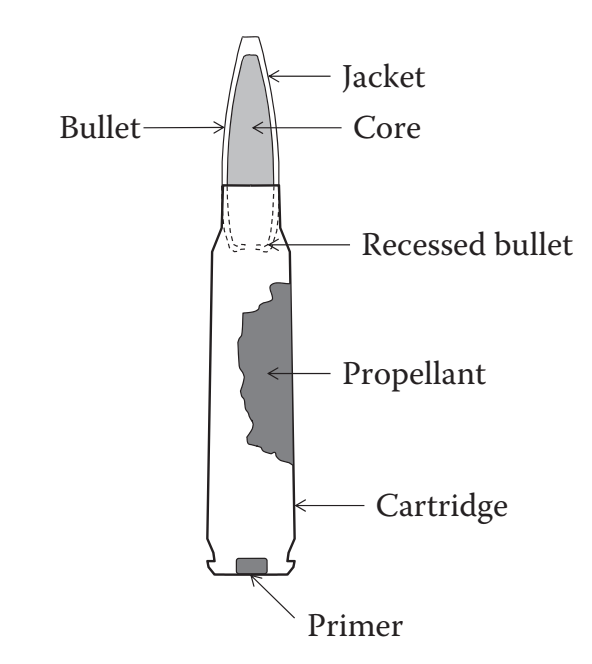
\includegraphics[width=0.5\linewidth]{images/projetil_inteiro.png}
	\label{fig:projetilinteiro}
	\fonte{\cite{Hazell}}
\end{figure}

Existem três grandes variáveis para o sucesso de um projetil, são elas sua velocidade de saída, seu material e sua geometria. O diâmetro destes projeteis aparece em milímetros ou em polegadas. Em milímetro as dimensões 7.62 e 5.56 são muito usadas, já em polegadas tem-se o .30 (7.62 milímetros)  e o .50 (12.7 milímetros) como exemplos. Ainda pertencendo a geometria o formato da ponta é de grande importância. As pontas esféricas são menos agressivas em relação às em ogiva ou cone.\\
Os materiais usados para a construção variam de acordo com a intenção do projetil. Os de menor poder penetrante são fabricados usando ligas de chumbo. Os de médio poder penetrante são fabricados de aço carbono ou aço carbono de baixa liga . Projeteis de alto poder de penetração são fabricados de um metal duro contendo carbeto de tungstênio em uma base de cobalto ou de ligas de aço altamente endurecíveis. A velocidade de saída pode variar muito entre os diferentes calibres, logo o limite considerado neste trabalho é na casa dos $ 2000 m/s $, baixo o suficiente para não haver ondas de choque em um metal ou cerâmica. \\


\subsection{A formação de orifício dúctil}
 O primeiro modo de penetração é a formação de um orifício dúctil, vide figura \ref{fig:buracoductil}. Ele é comum em placas dúcteis impactadas por projeteis pontiagudos. De acordo com \cite{Crouch} este mecanismo gera um furo de aspecto limpo e não retira massa do anteparo. O projetil age como um penetrador comparável à ponta de um durômetro quando este faz uma medição com sucesso, não havendo arredondamento de sua ponta. o ápice do projétil expulsa o material do anteparo para os lados de forma radial. A medida que o projetil avança há necessidade de abrir espaço para as secções que estão logo atrás do ápice. Este espaço é aberto pela deformação contínua do material do anteparo em maioria na direção radial e em minoria para outras direções normais à superfície do projétil. A maior parte destas deformações ocorre sob regime plástico, sendo assim a resistência dinâmica às tensões compressivas, em regime plástico, controlam a eficácia do material que falha desta forma. De acordo com \cite{Crouch} este é o modo de falha que traz a maior resistência a penetração enquanto apresenta os menores efeitos na face traseira do anteparo.
 
 \begin{figure}[H]
 	\centering
 	\caption{Formação de orifício dúctil.}
 	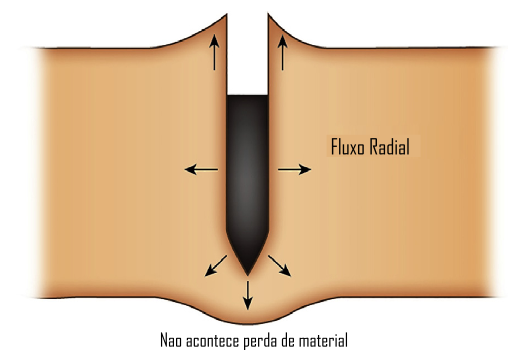
\includegraphics[width=0.5\linewidth]{images/Perfplast.png}
 	\label{fig:buracoductil}
 	\fonte{\cite{Crouch} traduzida pelo autor.}
 \end{figure}
 
 \subsection{O destacamento}
 
 O segundo modo é o "plugging" ou destacamento. Ele acontece, principalmente, quando o projétil apresenta ponta não aguda.  No momento subsequente ao contato entre projetil e anteparo há formação de um volume de partículas aceleradas que descrevem um cilindro na frente do projetil. As partículas localizadas fora deste volume não são aceleradas de forma significativa e é plausível considerar que permaneçam estacionárias em relação às do cilindro. Na área de fronteira entre as partículas aceleradas e não aceleradas ocorrem altas taxas de deformação cisalhante. De acordo com \cite{Crouch} já que o cisalhamento é extremamente localizado o material sofre pouca deformação plástica, logo sua absorção de energia é seriamente prejudicada. Existem materiais especificamente sensíveis a um tipo especial de destacamento que forma bandas finas de cisalhamento adiabático, nas quais o cisalhamento é ainda mais localizado fazendo com que a energia absorvida seja particularmente baixa. O nome dado a este fenômeno é cisalhamento adiabático e de acordo com \cite{Crouch} ainda não há um consenso sobre sua causa. O resultado do modo de falha destacamento é justamente o destacamento da porção de material logo a frente do projetil como visto na figura \ref{fig:furocilindro}. Este é um fenômeno considerado prejudicial em relação à absorção de energia, já que ocorre de forma localizada gastando pouca energia do projétil e  deve ser evitado. De acordo com \cite{Hazell} o destacamento ocorre com maior frequência quando a largura do anteparo e o diâmetro do projétil tem dimensão semelhante. Portanto como calibres mais comuns tem abaixo de $ 7.62mm $ chapas de $5$ a $ 8mm $ são as mais suscetíveis ao destacamento. Um ponto levantado por \cite{Crouch} é que o destacamento pode gerar um projetil secundário que deve ser contido. \\
 
   \begin{figure}[H]
 	\centering
 	\caption{Formação de um destacamento.}
 	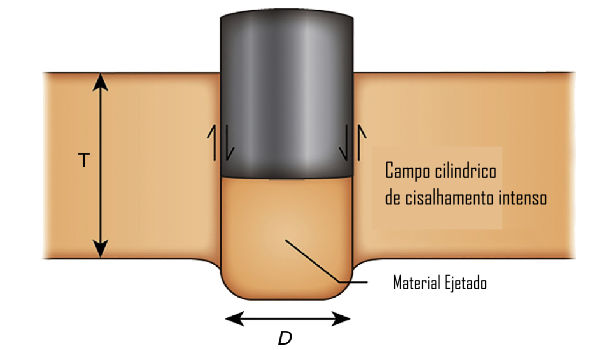
\includegraphics[width=0.5\linewidth]{images/plugging.png}
 	\label{fig:furocilindro}
 	\fonte{\cite{Crouch} traduzida pelo autor.}
 \end{figure}
 
 \subsection{A fratura conoidal e a cominuição}
 Este tipo de falha conjunta é encontrada em materiais duros como cerâmicos e vidros. \cite{Crouch} aponta que a fratura conoidal acontece em aços de ultra alta dureza, porém a cominuição não está presente. Na fratura conoidal a energia do projetil é transferida ao anteparo gerando trincas, chamadas hertzianas ou de hertz, que se propagam formando um cone adjacente à ponta do projetil, vide figura \ref{fig:hertz}. De acordo com \cite{Crouch} cones com maior ângulo são favoráveis ao desempenho balístico. O coeficiente de Poisson é a propriedade que mais tem mais influência sob este ângulo, maiores coeficientes de Poisson geram cones com ângulos maiores. \\
 
 A cominuição é caracterizada pela fratura do material formando várias partículas agudas de alta dureza, vide figura \ref{fig:cominuição}. A energia usada para o colapso do material não representa quantia significativa na redução da energia do projetil, porém a medida que este avança colide com as partículas formadas sendo erodido e perdendo massa. De acordo com \cite{neckel} a diminuição de massa ocorre até que as partículas do anteparo atinjam a velocidade do projetil  formando uma nuvem de partículas aceleradas. O processo de erosão descrito é responsável pela maior redução de energia em um anteparo de alta dureza que apresenta cominuição. Em algumas armaduras esta é a fonte principal de redução de energia do projetil, entretanto quando este tipo de falha está presente o sistema necessita de um material absorsor justaposto ao anteparo. Armaduras que usam anteparos cerâmicos normalmente possuem metais que são capazes de absorver tanto a energia residual do projetil quanto a energia da nuvem de partículas aceleradas pela colisão com o projetil.

 \begin{figure}[H]
 	\centering
 	\caption{Formação de trincas conoidais.}
 	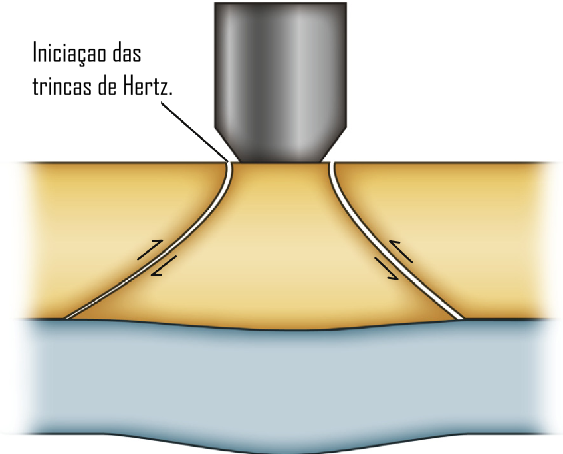
\includegraphics[width=0.5\linewidth]{images/hertz.png}
 	\label{fig:hertz}
 	\fonte{\cite{Crouch} traduzida pelo autor.}
 \end{figure}
 \begin{figure}[H]
 	\centering
 	\caption{Processo de cominuição.}
 	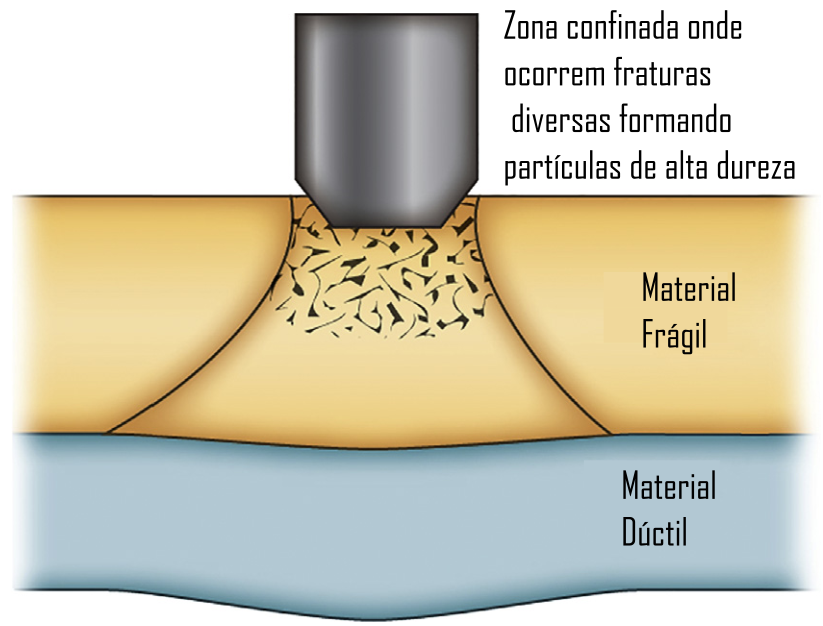
\includegraphics[width=0.5\linewidth]{images/comi.png}
 	\label{fig:cominuição}
 	\fonte{\cite{Crouch} traduzida pelo autor.}
 \end{figure}
 
 \section{As ondas de tensão}
 
 A formação de ondas de tensão acontece sempre que um objeto em movimento e um estacionário colidem. Em velocidades baixas as ondas de tensão são elásticas e aumentando a velocidade são formadas ondas de tensão plástica. Em velocidades muito  elevadas as ondas de choque são formadas, porém de forma geral tais velocidades estão fora do escopo deste trabalho.\\
 
 Quando solicitações quasi-estáticas são examinadas o ensaio de tração é feito para desenhar uma curva tensão vs deformação e este ensaio, quando feito de forma padrão, gera um estado uniaxial de tensão na peça. Uma curva tensão vs deformação em estado uniaxial de tensão é apresentada na figura \ref{fig:tensuniaxi}.
 
 \begin{figure}[H]
     \centering
     \caption{Curva tensão deformação em estado uniaxial de tensão.}
     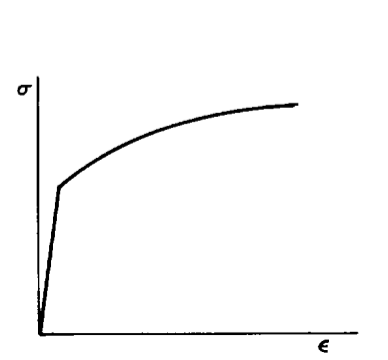
\includegraphics[width=0.5\linewidth]{images/tensuniaxial.png}
     \label{fig:tensuniaxi}
     \fonte{\cite{Zukas}}
 \end{figure}
 
 Porém quando o impacto em materiais é estudado o estado uniaxial de tensão não é mais conveniente, no sentido de que é difícil incitar tal estado em um impacto. O estado uniaxial de deformação é mais facilmente atingido, portanto este é o estado mais usado nestas situações. Este tipo de estado gera curvas como as da figura \ref{fig:defuniaxi}.
 
 \begin{figure}[H]
     \centering
     \caption{Curva tensão deformação em estado uniaxial de deformação.}
     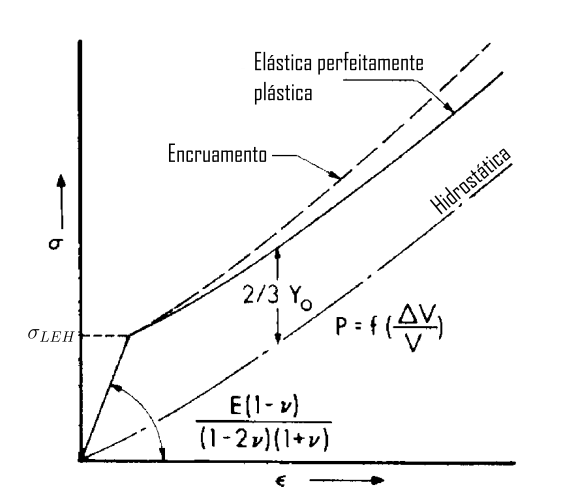
\includegraphics[width=0.5\linewidth]{images/defuniaxial.png}
     \label{fig:defuniaxi}
     \fonte{\cite{Zukas} traduzido pelo autor.}
 \end{figure}
 
 Veja que na figura \ref{fig:defuniaxi} também está presente o estado de tensões hidrostáticas. Com o acréscimo da tensão chegará um ponto onde a curva que considera a resistência do material será irrelevante numericamente. Este é o tipo de situação na qual os códigos de propagação de ondas foram criados, por isso o nome hidrocódigo surgiu. \\
 Na curva descrita pelo material estão representados dois cenários. Num o material apresenta comportamento perfeitamente plástico, noutro há encruamento. Veja que aqui o encruamento originalmente foi apresentado pelo autor \cite{Zukas} como originado apenas pela deformação, mas materiais cerâmicos tendem a apresentar aumento da resistência devido ao aumento da pressão também. \\
 
 Um ponto importante da curva é o limite elástico de Hugoniot ou $\sigma_{LEH} $. Ele marca a mudança de comportamento de elástico para plástico e é também a amplitude da onda elástica quando ondas plásticas estão presentes. Doravante onda elástica, onda plástica e onda de choque querem dizer onda de tensão elástica e por conseguinte. A velocidade da onda elástica é calculada usando a inclinação da reta em regime elástico seguindo a expressão
 
 \begin{equation} \label{eq:ondaelasticavel}
     c_{e} = \sqrt{\ddfrac{E(1- \nu )}{\rho_r (1 - 2\nu )(1+ \nu)}} 
 \end{equation}
 
 Caso as tensões forem superiores a \gls{hugoniot} a onda elástica se propagará com a velocidade descrita na equação \ref{eq:ondaelasticavel} e uma ou algumas ondas elásticas se propagarão de acordo com a seguinte equação
 
 \begin{equation} \label{eq:ondaplasticavel}
     c_{p} = \sqrt{\frac{1}{\rho} \frac{d \sigma}{d \varepsilon}}
 \end{equation}
 
 Portanto a velocidade de uma onda plástica está associada a derivada da tensão pela deformação no regime plástico. Quando o nível de deformação é muito alto esta derivada tende a ter valor muito elevado, aumentando muito a velocidade da onda em relação às anteriores. A imagem \ref{fig:elastochoque} mostra  o comportamento esperado de uma curva de tensão deformação em estado uniaxial de deformação até o estado de choque. \\
 
 
 \begin{figure} [H]
     \centering
     \caption{Gráfico dos regimes elástico, elastoplástico e de choque.}
     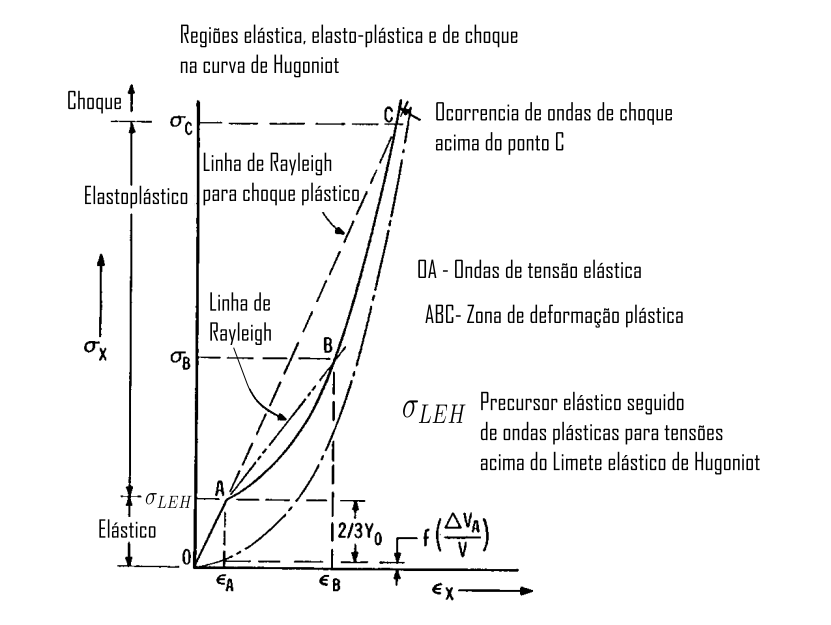
\includegraphics[width=0.5\linewidth]{images/elasticplasticshock.png}
     \label{fig:elastochoque}
     \fonte{\cite{Zukas} traduzido pelo autor.}
 \end{figure}
 
 O critério principal para o acontecimento de uma onda de choque é que a velocidade da onda plástica mais rápida seja suficiente para alcançar as ondas plásticas anteriores formando uma descontinuidade na curva que descreve a pressão ao longo do tempo, ou da distância, assim como é visto na figura \ref{fig:buildshock}. De acordo com \cite{Zukas} este tipo de acontecimento é esperado em impactos com velocidade superiores a $2000 m/s$, já \cite{Hazell} afirma que isto acontece quando a taxa de penetração do projetil é maior do que a velocidade do som no meio. A tabela \ref{tab:veldosom} mostra a velocidade do som em alguns meio comuns no âmbito da ciência balística. Veja que de acordo com \cite{Hazell} uma onda de choque se formaria apenas em velocidades muito altas em meios sólidos. Para armamentos pequenos tais velocidades são absurdas, porém \cite{Hazell} afirma que projeteis lançados por explosivos podem chegar aos $11000 m/s$.
 
  \begin{figure} [H]
     \centering
     \caption{Formação de uma onda de choque.}
     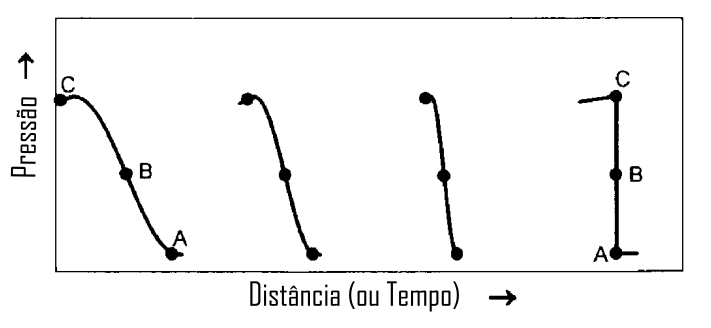
\includegraphics[width=0.5\linewidth]{images/buildshock.png}
     \label{fig:buildshock}
     \fonte{\cite{Zukas} traduzido pelo autor.}
 \end{figure}
 
 \begin{table}[H]
     \centering
     \caption{Velocidade do som em alguns materiais}
\begin{tabular}{|l|l|l}
\cline{1-2}
\textbf{Meio} & \textbf{Velocidade do som (m/s)} &  \\ \cline{1-2}
Ar            & 330                              &  \\ \cline{1-2}
Alumina       & 9900                             &  \\ \cline{1-2}
Alumínio      & 6300                             &  \\ \cline{1-2}
Aço carbono   & 5920                             &  \\ \cline{1-2}
Titânio       & 6100                             &  \\ \cline{1-2}
\end{tabular}
     \label{tab:veldosom}
     \fonte{\url{http://www.classltd.com/sound_velocity_table.html}}
 \end{table}
 
 
 \subsection{A impedância elástica.} (Talvez seja melhor retirar toda esta subseção. Pois ela chega em uma relação que apenas \cite{Hazell} cita como importante.)
 
 Quando duas placas estão em contato e uma delas sofre um impacto uma onda de tensão se propaga em direção à outra. Para manter a simplicidade, apenas ondas longitudinais serão consideradas. A onda original, chamada de incidente, é refletida e transmitida de acordo impedância elástica de cada material. A figura \ref{fig:ondasincierefle} apresenta  a direção de propagação das ondas longitudinais em questão. A tensão na interface estará em equilíbrio, de forma que
 
 \begin{equation} \label{eq:equitensao}
     \sigma_I + \sigma_R = \sigma_T
 \end{equation}
 
 onde  $ \sigma_I $ é a tensão incidente, $ \sigma_r $ a refletida e $ \sigma_T $ a transmitida. De acordo com \cite{Hazell} considera-se que não há espaços na interface e nem superposição de material. Por conta de tal consideração  as velocidades das partículas carregadas excitadas pelas ondas se comporta da seguinte maneira
 
 \begin{equation} \label{eq:equivel}
     u_{pI} + u_{pR} = u_{pT}
 \end{equation}
 
 Na qual $u_{p}$ significa velocidade da partícula e os  índices $I$, $R$ e $T$ mantém seu significado denotando incidente, refletido e transmitido. A velocidade da partícula pode ser calculada da seguinte maneira
 
 \begin{equation} \label{eq:calculodavel}
     u_p = \ddfrac{\sigma}{\sqrt{\rho_r E^{p/e}}}
 \end{equation}

Onde o símbolo $ E^{p/e} $ significa módulo de elasticidade ou o módulo elastoplastico. O módulo de elasticidade serve para situações elásticas e o elastoplastico para ondas plásticas.\\
 
 \begin{figure}[H]
     \centering
     \caption{Representação da reflexão e transmissão de ondas tensão.}
     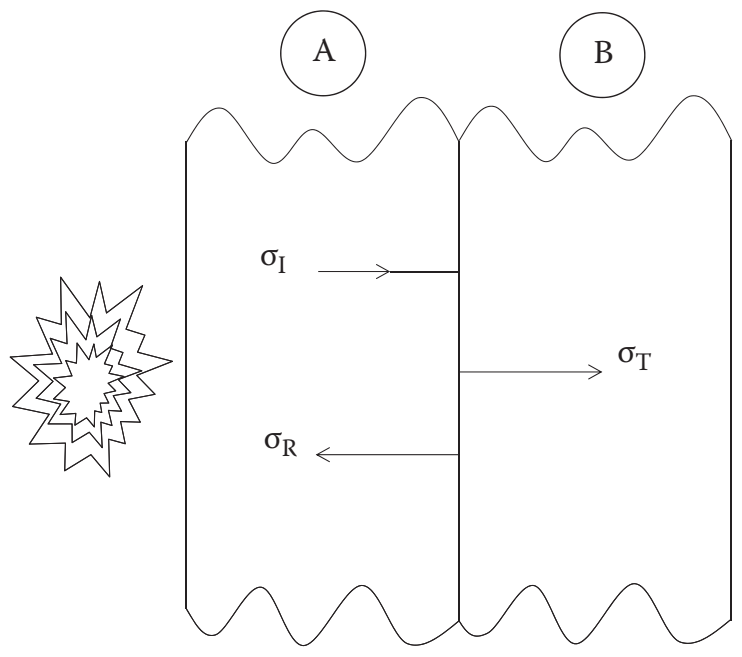
\includegraphics[width=0.5 \linewidth]{images/ondasincirefle.png}
     \label{fig:ondasincierefle}
     \fonte{\cite{Hazell}}
 \end{figure}
 
Considerando um impacto que não provocará inelasticidade. Ao aplicar \ref{eq:calculodavel} em \ref{eq:equivel} a seguinte expressão é obtida para dois materiais $A$  e  $B$ dispostos como na figura \ref{fig:ondasincierefle}.

\begin{align} \label{eq:velocitensao}
    u_{pI} = \ddfrac{\sigma_I}{\sqrt{E_A\rho_A}}, && u_{pR} = \ddfrac{-\sigma_R}{\sqrt{E_A\rho_A}}, && u_{pI} = \ddfrac{\sigma_T}{\sqrt{E_B\rho_B}}
\end{align}
 
  
 Agora resolvendo \ref{eq:velocitensao} e \ref{eq:equitensao} simultaneamente a seguinte expressão para a razão entre tensão refletida e transmitida é encontrada.
 
 \begin{equation}
     \ddfrac{\sigma_R}{\sigma_I} = \ddfrac{\sqrt{E_B \rho_B} - \sqrt{E_A \rho_A}}{\sqrt{E_B \rho_B} + \sqrt{E_A \rho_A}}
 \end{equation}
 
Usando esta relação, de acordo com \cite{Hazell} é possível otimizar o desempenho de materiais cerâmicos por meio de comparação entre dois metais de suporte diferentes. O melhor material para ser usado com a cerâmica é aquele que faz com que as tensões refletidas para sejam as menores possíveis. o cenário ótimo é aquele no qual a tensão refletida é compressiva. É importante apontar que o sinal das tensões é invertido na literatura balística, portanto tensões trativas tem sinal negativo. \\

Mesmo que as tensões refletidas sejam compressivas e portanto o acoplamento entre a cerâmica e o metal seja ótimo, ainda assim a cerâmica sofrerá fratura por conta das tensões trativas que são refletidas pela superfície livre da placa metálica. O ponto aqui é atrasar a fratura aumentando o desempenho da cerâmica quanto à penetração inicial.

\section{A aplicação de cerâmicas como classe de materiais de proteção.}

De acordo com \cite{Crouch} os cerâmicos são a classe de materiais mais importantes na blindagem moderna. Tanto óxidos quanto não óxidos tem importância elevada no meio, já que são ótimos disruptores de projéteis e portanto oferecem uma boa proteção ao impacto. Neste contexto estão inseridos os vidros, as cerâmicas transparentes e as translucidas, que desempenham funções outras, além da proteção balística. Este trabalho não abordará as cerâmicas transparentes, translucidas ou vidros. O foco aqui são cerâmicos opacos, cuja função é exclusivamente fornecer proteção.\\

A configuração padrão quando cerâmicas são usadas para proteção é a de dupla camada, sendo a primeira cerâmica e a segunda metálica. A função da cerâmica é erodir e fraturar o projetil reduzindo sua energia. De acordo com \cite{neckel_hotza_stainer_janssen_al-qureshi_2013} a cerâmica é responsável pela absorção de $85\%$ da energia na configuração usada por eles. \\

\subsection{Fatores importantes na aplicação de cerâmicas opacas.}

Mark Wilkins foi um dos grandes contribuidores para o entendimento da aplicação de cerâmicas em sistemas de blindagem. Sua série de relatórios, na qual o primeiro é \cite{firstreport}, aponta que a rigidez é de grande importância para o desempenho balístico em sistemas baseados no alumínio como placa de absorção. O modelo computacional de Wilkins foi um dos, senão o primeiro, a caracterizar fases importantes da penetração em materiais cerâmicos. \\

De acordo com \cite{reijel} é importante que a dureza da cerâmica seja superior à do projétil e \cite{Crouch} diz que é desejável que a razão dureza/densidade seja alta. Esta razão está ligada ao cone de fratura, já que quanto maior a base do cone melhor é o desempenho balístico. Quanto maior a espessura da cerâmica maior será a base do cone, então cerâmicas de menor densidade podem ser usadas em maior espessura, mantendo baixa a densidade de área. No âmbito de impacto balístico quando se diz densidade de área quer se dizer o resultado da densidade do material pela espessura da placa usada.  \\

\cite{Crouch} diz que não há consenso de um destacamento de propriedades medidas de forma estática que fazem com que o desempenho balístico aumente. Porém ele cita que as seguintes propriedades são importantes

\begin{itemize}
    \item Dureza : Sempre acima da dureza do projetil. Em geral acima de $10$ $GPa$
    \item Densidade: Deve ser a menor possível.
    \item Resistência em ensaio de flexão: Acima de $350$ $MPa$ é desejada.
\end{itemize}

Além disso \cite{kaufmann_cronin_worswick_pageau_beth_2003} discorre sobre a influência de algumas propriedades dos materiais cerâmicos em seu comportamento balístico usando experimentos com alumina $99.9 \%$ (CERAMOR), alumina modificada(CERAMOR-Z), carbeto de silício (Hexoloy) e carbeto de boro (Ceralloy
546). Tanto o carbeto de silício quanto o carbeto de boro são produtos comercias, já as aluminas não foram encontradas e o autor não cita a mudança realizada na alumina modificada. Porém os resultados são úteis mesmo sem o conhecimento da composição da alumina modificada. Os testes feitos por ele são de Profundidade de penetração em velocidades de $750$, $850$ e $910 m/s$ usando uma liga de alumínio $6061-T6$ como material de apoio.\\

As propriedades das cerâmicas testadas foram normalizadas usando a alumina $99.9\%$ como padrão, a figura \ref{fig:propceramis} apresenta estes resultados.    \footnote{A imagem apresentava qualidade muito baixa no artigo original, portanto foi necessário refaze-la, sem alteração qualquer nos dados apresentados, para o conforto do leitor deste texto.}

\begin{figure}
    \centering
    \caption{Propriedades das cerâmicas normalizadas pela alumina $ 99.9 \% $}
    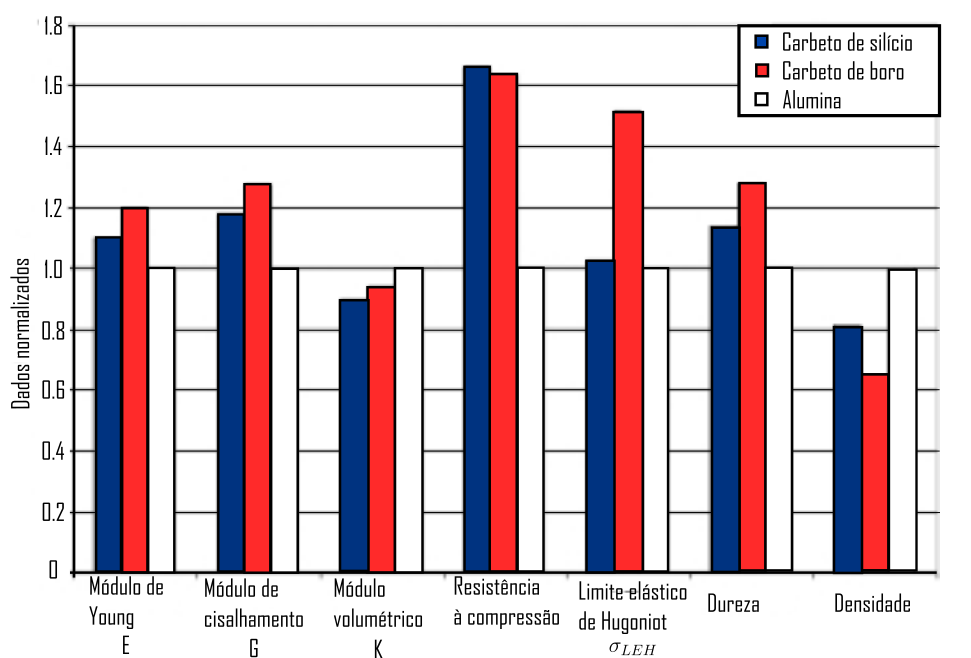
\includegraphics[width=0.8\linewidth]{images/propceramis.png}
    \label{fig:propceramis}
    \fonte{\cite{kaufmann_cronin_worswick_pageau_beth_2003} refeita e traduzida pelo autor.}
\end{figure}


Resistência à compressão: De acordo com \cite{shockey_marchand_skaggs_cort_burkett_parker_1990} ela é responsável pela resistência inicial da cerâmica a um projetil. No trabalho de \cite{kaufmann_cronin_worswick_pageau_beth_2003} foi observado que a resistência à compressão dos carbetos usados é semelhante e maior que a da alumina. O carbeto de silício apresenta melhores resultados em todos as velocidades usadas por \cite{kaufmann_cronin_worswick_pageau_beth_2003}, portanto ele conclui que ,devido aos dois carbetos apresentarem densidade de área semelhante, a resistência à compressão não é um fator dominante neste caso. Uma leitura diferente da feita pelo autor é que a resistência à compressão domina apenas a parte inicial da penetração e depois desta outras propriedades passam a dominar o evento. A motivação para tal é o resultado superior dos carbetos em relação à alumina. \\

Dureza: \cite{reijel} afirma que a dureza da cerâmica deve ser sempre maior que a do projetil e valores acima disto não são necessários. A importância da dureza está na erosão da ponta do projetil, dado que uma das partes iniciais do processo de penetração em uma cerâmica é justamente esta erosão. O processo de penetração na integra é revisado na seção seguinte.

Módulo de Young, de cisalhamento e volumétrico: O carbeto de boro tem o maior módulo de Young entre as cerâmicas testadas e portanto, dado que as densidades são semelhantes, possui a maior impedância elástica. Por ter maior impedância este deveria ter vantagem quanto ao desempenho balístico, pois as ondas refletidas seriam menos prejudiciais. Mesmo o carbeto de boro tendo uma vantagem esperada, o carbeto de silício apresentou resultados melhores em todos os testes. Quanto ao módulo de cisalhamento novamente o carbeto de boro tem o maior, porém  não desempenha os melhores resultados. O módulo volumétrico de todos as cerâmicas testadas são semelhantes. \cite{kaufmann_cronin_worswick_pageau_beth_2003} conclui que os módulos parecem não ter afetado os testes realizados por ele.

Limite elástico de Hugoniot: Aqui novamente o carbeto de boro é superior, porém é superado pelo carbeto de silício que tem  limite semelhante à alumina testada. \cite{kaufmann_cronin_worswick_pageau_beth_2003} conclui que o limite elástico de Hugoniot parece ter pouca influência na resistência de materiais cerâmicos ao impacto.

\subsection{Os mecanismos de absorção de energia e o modo de falha}

O processo de falha de uma cerâmica impactada por um projetil é apresentado passo a passo na figura \ref{fig:processo}.
\cite{Crouch} afirma que todas as fraturas relacionadas com as trincas de hertz e a cominuição são responsáveis pela diminuição de apenas $1\%$ da energia do impacto. Grande parte da energia do projetil é consumida através da erosão, portanto a cominuição é extremamente importante. De acordo com \cite{anderson} é uma das partes mais importantes do processo e é um dos fatores mais importantes na penetração. Outra indicação disto é trazida por \cite{holmquist_johnson_2002} que faz comparações da penetração entre um modelo que considera ou não a falha do material. Nas simulações onde o material não falha os valores previstos são irreais. Naquelas onde a porção do material abaixo do material falha gradativamente, de acordo com o modelo de Johnson-Holmquist, a penetração é corretamente prevista. De certa forma este é o caminho encontrado para simular a cominuição, já que seria muito complexo replicar o fenômeno em si. \\

De acordo com \cite{Crouch} é extremamente importante que todos os passos da figura \ref{fig:processo} ocorram na ordem descrita. A presença de porosidades nas adjacências do impacto é algo a ser evitado ao máximo, já que esta pode reduzir muito a resistência do cerâmico em compressão. \cite{Crouch} realizou experimentos de impactos em locais onde trincas originadas em impactos anteriores estavam presentes. Foi observado que houve redução de $9\%$ no desempenho balístico. 



\begin{figure}
    \centering
    \caption{Processo de penetração de um projetil em uma cerâmica suportada por um laminado.}
    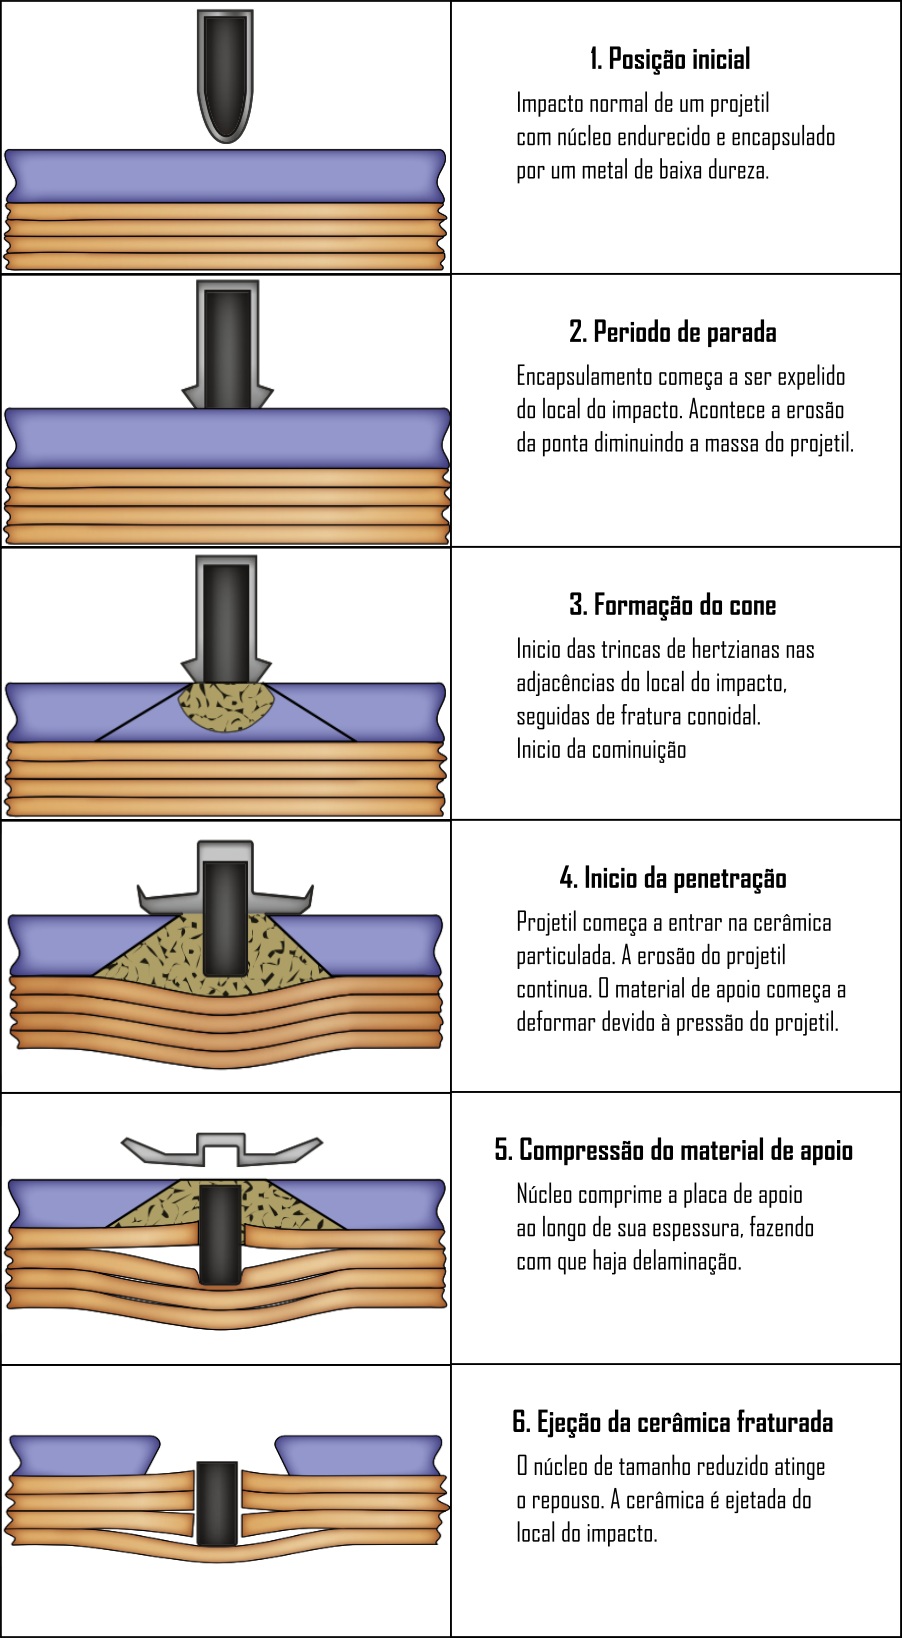
\includegraphics[width=0.7\linewidth]{images/processodepenetra.png}
    \label{fig:processo}
    \fonte{\cite{Crouch} traduzida pelo autor.}
\end{figure}


 
% ---

% ---
% 3 - Conclusão
% ---
%\phantompart
% ----------------------------------------------------------
\chapter{Conclusão}
% ----------------------------------------------------------

O ponto de partida para o estudo computacional dos fenômenos de impacto é a clássica mecânica do contínuo. A primeira parada dentro deste campo que foi apenas superficialmente visitado é a cinemática, portanto a descrição do movimento e das deformações. Mesmo sem uma apresentação formal do cálculo e da álgebra tensorial estes foram usados para andar por entidades tensoriais que descrevem os meios contínuos. A introdução de um conceito que não é apresentado durante os cursos de graduação em engenharia, que é a existência dos tensores de deformação finitesimal, é destacado como a parte mais importante da revisão da cinemática. Além da apresentação a importância do tensor \gls{E} foi demonstrada usando gráficos do comportamento deste em relação à sua versão linearizada \gls{eps}. \\

Depois da cinemática foram apresentados os princípios termomecânicos básicos. Eles conduzem todos os processos termomecânicos, de acordo com a mecânica do contínuo. A importância de conhecer estes princípios é semelhante à de conhecer as regras de um jogo que está sendo jogado, já que eles definem o que é ou não é permitido fisicamente. Estes princípios são todos válidos inclusive quando ondas de choque estão presentes no meio, embora sua formulação possa sofrer mudança. O conceito de ondas de choque foi introduzido no último assunto do trabalho, porém veja como a presença ou não delas afeta inclusive as considerações mais básicas, que foram apresentadas logo de início. \cite{gurtin_fried_anand_2013} faz a derivação dos mesmos conceitos termodinâmicos básicos na presença de ondas de choque, caso o leitor tenha interesse. \\ 

Dentro da revisão dos princípios termodinâmicos está um dos teoremas mais importantes e impactantes na mecânica dos sólidos, que é o teorema de Cauchy. Ele não só é fundamental para a solução do balanço de momento linear, quanto possibilita o o entendimento dos efeitos de uma entidade tão misteriosa chamada força. De acordo com \cite{gurtin_fried_anand_2013} aqueles que acreditam que a definição e o entendimento da força é algo trivial deveriam ler as obras literárias do período logo após newton. O autor inclusive cita uma frase de D'Alembert quando falava sobre as forças de newton. "Elas são entidades metafísicas obscuras capazes tão somente de espalhar escuridão sobre uma ciência inerentemente clara". Há um grande espectro de técnicas capazes de resolver o balanço de momento linear em domínios de  diferentes complexidades, porém o método dos elementos finitos é o escolhido pela indústria de defesa e também por este trabalho. A solução por elementos finitos começa pela formulação da chamada forma fraca, que gera um relaxamento na necessidade de continuidade do campo de deslocamentos. Depois disso a discretização espacial é responsável por segmentar o corpo em elementos que interagem e formam um sistema algébrico a ser resolvido no espaço. A partir daí a discretização no tempo tem responsabilidade de propagar a solução deste sistema algébrico no tempo. O resultado do sistema discretizado tanto no espaço quanto no tempo é a descrição de campos como a deformação, a tensão e o dano no material. Com esta descrição é possível confirmar ou refutar hipóteses. \\

A formulação apresentada usou a lei de Hooke como modelo constitutivo para simplificar o processo de derivação das expressões. Em um código de propagação de ondas comercial são usados muitos outros modelos para representar a tensão em função das variáveis internas do material. A plasticidade computacional foi introduzida para mostrar o ambiente teórico onde são encaixados os modelos constitutivos mais usados em simulações de impacto balístico. Então estes modelos foram apresentados, destes destacam-se o modelo de Johnson-Cook para metais e os de Johnson-Holmquist para cerâmicos, pois são simples e extremamente úteis.\\

Para realizar uma simulação basta um programa de elementos finitos em conjunto com um modelo constitutivo bem definido. Isto é fornecido por todos os programas comerciais competentes. Agora para realizar uma simulação útil são necessárias a calibração dos parâmetros da simulação e a correta interpretação de seus resultados. Tanto a interpretação quanto a calibração necessitam conhecimento do fenômeno que está acontecendo. Este conhecimento é muito mais crítico quando o impacto balístico é o fenômeno. \cite{Zukas} cita o campo como uma ciência com toques artísticos, já que usando o mesmo código para simular o mesmo fenômeno são possíveis inúmeros resultados finais, devido à diversidade de possíveis ajustes que muitas vezes precisam ser ajustados de acordo com a experiência do usuário. Além disso a simulação é apenas uma ferramenta para a pesquisa, o trabalho de \cite{kaufmann_cronin_worswick_pageau_beth_2003} mostra a dificuldade de se tirar conclusões, mesmo com a experimentação do fenômeno. Sendo assim o conhecimento dos princípios básicos e do que se deve esperar é primordial para uma simulação, já que o computador sempre apresentará resultados e cabe ao analista saber se estes são ou não confiáveis. \\
% ---

% ----------------------------------------------------------
% ELEMENTOS PÓS-TEXTUAIS
% ----------------------------------------------------------
\postextual
% ----------------------------------------------------------

% ----------------------------------------------------------
% Referências bibliográficas
% ----------------------------------------------------------
\begingroup
    \SingleSpacing\printbibliography[title=REFERÊNCIAS]
\endgroup

% ----------------------------------------------------------
% Glossário
% ----------------------------------------------------------
%
% Consulte o manual da classe abntex2 para orientações sobre o glossário.
%
%\glossary

% ----------------------------------------------------------
% Apêndices
% ----------------------------------------------------------

% ---
% Inicia os apêndices
% ---
%\begin{apendicesenv}
%	\partapendices* 
%	\input{aftertext/apendice_a}
%\end{apendicesenv}
% ---


% ----------------------------------------------------------
% Anexos
% ----------------------------------------------------------

% ---
% Inicia os anexos
% ---
%\begin{anexosenv}
%	\partanexos*
%	\input{aftertext/anexo_a}
%\end{anexosenv}

%---------------------------------------------------------------------
% INDICE REMISSIVO
%---------------------------------------------------------------------
%\phantompart
%\printindex
%---------------------------------------------------------------------

\end{document}
